\documentclass[12pt,]{article}
%\usepackage{lmodern}  Melissa removed to deal with font rendering issue
\usepackage{amssymb,amsmath}
\usepackage{ifxetex,ifluatex}
\usepackage{fixltx2e} % provides \textsubscript

%Melissa removed the following section to deal with font rendering issue
%\ifnum 0\ifxetex 1\fi\ifluatex 1\fi=0 % if pdftex
%  \usepackage[T1]{fontenc}
%  \usepackage[utf8]{inputenc}
%%\else % if luatex or xelatex
%  \ifxetex
%    \usepackage{mathspec}
%  \else
%    \usepackage{fontspec}
%  \fi
%  \defaultfontfeatures{Ligatures=TeX,Scale=MatchLowercase}
%  \newcommand{\euro}{€}
%%%%%%\fi

% use upquote if available, for straight quotes in verbatim environments
\IfFileExists{upquote.sty}{\usepackage{upquote}}{}
% use microtype if available
\IfFileExists{microtype.sty}{%
\usepackage{microtype}
\UseMicrotypeSet[protrusion]{basicmath} % disable protrusion for tt fonts
}{}
\usepackage[margin=1in]{geometry}
\usepackage{hyperref}
\PassOptionsToPackage{usenames,dvipsnames}{color} % color is loaded by hyperref
\hypersetup{unicode=true,
            pdftitle={Status of Petrale sole (Eopsetta jordani) along the US west coast in 2019},
            pdfborder={0 0 0},
            breaklinks=true}
\urlstyle{same}  % don't use monospace font for urls
\usepackage{graphicx,grffile}
\makeatletter
\def\maxwidth{\ifdim\Gin@nat@width>\linewidth\linewidth\else\Gin@nat@width\fi}
\def\maxheight{\ifdim\Gin@nat@height>\textheight\textheight\else\Gin@nat@height\fi}
\makeatother
% Scale images if necessary, so that they will not overflow the page
% margins by default, and it is still possible to overwrite the defaults
% using explicit options in \includegraphics[width, height, ...]{}
\setkeys{Gin}{width=\maxwidth,height=\maxheight,keepaspectratio}
\setlength{\parindent}{0pt}
\setlength{\parskip}{6pt plus 2pt minus 1pt}
\setlength{\emergencystretch}{3em}  % prevent overfull lines
\providecommand{\tightlist}{%
  \setlength{\itemsep}{0pt}\setlength{\parskip}{0pt}}
\setcounter{secnumdepth}{5}

%%% Use protect on footnotes to avoid problems with footnotes in titles
\let\rmarkdownfootnote\footnote%
\def\footnote{\protect\rmarkdownfootnote}

%%% Change title format to be more compact
\usepackage{titling}

% Create subtitle command for use in maketitle
\newcommand{\subtitle}[1]{
  \posttitle{
    \begin{center}\large#1\end{center}
    }
}

\setlength{\droptitle}{-2em}
  \title{Status of Petrale sole (\emph{Eopsetta jordani}) along the US west coast
in 2019}
  \pretitle{\vspace{\droptitle}\centering\huge}
  \posttitle{\par}
  \author{}
  \preauthor{}\postauthor{}
  \date{}
  \predate{}\postdate{}


% This file contains all of the LaTeX packages you may need to compile the document
% Documentation for each package can be found onlines
\usepackage{tabularx}                                             % table environment providing flexibility
\usepackage{caption}                                              % for creating captions  
\usepackage{longtable}                                            % allows tables to span multiple pages
\usepackage{tabu}
\usepackage{rotating}                                             % allows for sideways tables
%\usepackage{float}                                                % floating environments; may not need in rmarkdown
\usepackage{placeins}                                             % keeps floats from moving
\usepackage{floatrow}                                             % package to put table captions at the top
\floatsetup[table]{capposition = top}                             % line to put captions at the top of pander tables
\usepackage{indentfirst}                                          % indents first paragraph of a section
\usepackage{mdwtab}                                               % continued float multi-page figure
\usepackage{enumerate}                                            % create lists
\usepackage{hyperref}                                             % highlight cross references
\hypersetup{colorlinks=true, urlcolor=blue, linktoc=page, linkcolor=blue, citecolor=blue} %define referencing colors
%\usepackage{makebox}                                             % make boxes around text
\usepackage[usenames,dvipsnames]{xcolor}                          % color name options
%\usepackage[space]{grffile}                                      % spaces in file name path
\usepackage{soul}                                                 % highlight text
\usepackage{enumitem}                                             % numbered lists
%\usepackage{lineno}                                               % Line numbers; comment out for final
\usepackage{upquote}                                              % produce grave accent in latex
\usepackage{verbatim}                                             % produces verbatim results
\usepackage{fancyvrb}                                             % verbatim in a box
%\usepackage{draftwatermark}                                      % places Draft watermark in background; comment out for final
\usepackage{textcomp}                                             % fixes error with packages interfering
\usepackage{lscape}                                               % rotate pages - to allow for landscape longtables
%\pdfinterwordspaceon                                             % fix loss of inter word spacing
\usepackage{cmap}                                                 % fix mapping characters to unicode
\RequirePackage[linewidth = 1]{pdfcomment}                        % pdf comments
\RequirePackage[l2tabu, orthodox]{nag}                            % checks packages related to the accessibility?
%\usepackage[inline]{showlabels}                                   % show table and figure labels; comment out for final
%\RequirePackage[tagged]{accessibilityMeta}


%\linenumbers                                                      % specify use of line numbers


\definecolor{light-gray}{gray}{.85}                               % define light-gray as a color
%\usepackage[tagged]{accessibility-meta}

 
%\showlabels[\color{mred}]{label}

% Redefines (sub)paragraphs to behave more like sections
\ifx\paragraph\undefined\else
\let\oldparagraph\paragraph
\renewcommand{\paragraph}[1]{\oldparagraph{#1}\mbox{}}
\fi
\ifx\subparagraph\undefined\else
\let\oldsubparagraph\subparagraph
\renewcommand{\subparagraph}[1]{\oldsubparagraph{#1}\mbox{}}
\fi

\begin{document}
\maketitle


\begin{center}
\thispagestyle{empty}


\vspace{.5cm}

%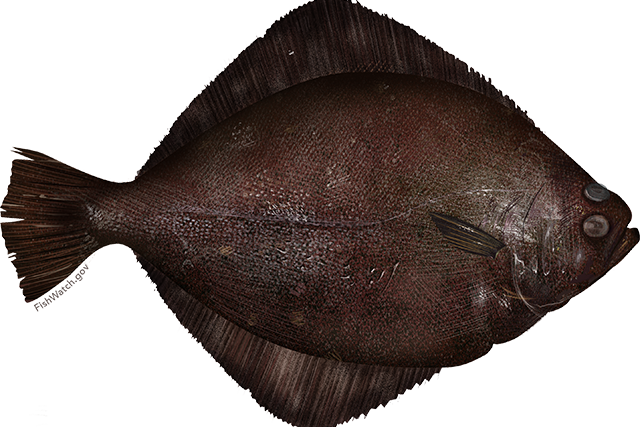
\includegraphics{petrale_sole}~\\[0.5cm]
%\pdftooltip{\includegraphics{Sebastes_alutus}}{This is a fish.}



Chantel R. Wetzel\textsuperscript{1}\\


\vspace{.5cm}

\small
\textsuperscript{1}Northwest Fisheries Science Center, U.S. Department of Commerce, National Oceanic and Atmospheric Administration, National Marine Fisheries Service, 2725 Montlake Boulevard East, Seattle, Washington 98112\\

\vspace{.3cm}





\vspace{1cm}

\vfill
June 2019


\vspace{.3cm}
%Bottom of the page
%{\large \today}

\newpage

\vspace{3cm}

Please cite as:\\

Wetzel, C.R. 2019. Status of Petrale sole (\textit{Eopsetta jordani}) along the US west coast in 2019. Pacific Fishery Management Council, 7700 Ambassador Place NE, Suite 200, Portland, OR 97220. 

\vspace{3cm}

\maketitle






\pagenumbering{roman}
\setcounter{page}{1}
\end{center}

{
\setcounter{tocdepth}{4}
\tableofcontents
}
\setlength{\parskip}{5mm plus1mm minus1mm} \pagebreak

\setcounter{page}{1} \renewcommand{\thefigure}{\alph{figure}}
\renewcommand{\thetable}{\alph{table}}

\section*{Executive Summary}\label{executive-summary}
\addcontentsline{toc}{section}{Executive Summary}

\subsection*{Stock}\label{stock}
\addcontentsline{toc}{subsection}{Stock}

This assessment reports the status of the Petrale sole
(\emph{Eopsetta jordani}) off U.S. coast of California, Oregon, and
Washington using data through 2018. While petrale sole are modeled as a
single stock, the spatial aspects of the coast-wide population are
addressed through geographic separation of data sources/fleets where
possible. There is currently no genetic evidence suggesting distinct
biological stocks of petrale sole off the U.S. coast. The limited
tagging data available to describe adult movement suggests that petrale
sole may have some homing ability for deep water spawning sites but also
have the ability to move long distances between spawning sites,
inter-spawning season, as well as seasonally.

\subsection*{Landings}\label{landings}
\addcontentsline{toc}{subsection}{Landings}

While records do not exist, the earliest catches of Petrale sole are
reported in 1876 in California and 1884 in Oregon. In this assessment,
fishery removals have been divided among 4 fleets: 1) winter North
trawl, 2) summer North trawl, 3) winter South trawl, and 4) summer South
trawl. Landings for the North fleet are defined as fish landed in
Washington and Oregon ports. Landings for the South fleet are defined as
fish landed in California ports. Recent annual catches during 1981-2014
range between 749-2,903 mt (Table XX, Figure XX). Petrale sole are
caught nearly exclusively by trawl fleets; non-trawl gears contribute
less than 3\% of the catches. Based on the 2005 assessment, annual catch
limits (ACLs) were reduced to 2499 mt for 2007-2008. Following the 2009
assessment ACLs were further reduced to a low of 976 mt for 2011 and
have subsequently increased to a high value of 3,136 for 2017. From the
inception of the fishery through the war years, the vast majority of
catches occurred between March and October (the summer fishery), when
the stock is dispersed over the continental shelf. The post-World War II
period witnessed a steady decline in the amount and proportion of annual
catches occurring during the summer months (March-October). Conversely,
Petrale sole catch during the winter season (November-February), when
the fishery targets spawning aggregations, has exhibited a steadily
increasing trend since the 1940s. From the mid-1980s through the early
2000s, catches during the winter months were roughly equivalent to or
exceeded catches throughout the remainder of the year, whereas during
the past 10 years the relative catches during the winter and summer have
been more variable across years (Figure XX). Petrale sole are a
desirable market species and discarding has historically been low.

\begin{table}[ht]
\centering
\caption{Landings (mt) for the past 10 years for Petrale sole by source.} 
\label{tab:Exec_catch}
\begin{tabular}{l>{\centering}p{0.7in}>{\centering}p{0.7in}>{\centering}p{0.7in}>{\centering}p{0.7in}>{\centering}p{0.7in}}
  \hline
Year & Winter (N) & Summer (N) & Winter (S) & Summer (S) & Total Landings \\ 
  \hline
2009 & 846.71 & 641.75 & 469.66 & 250.38 & 2208.49 \\ 
  2010 & 258.09 & 292.34 & 77.60 & 120.95 & 748.98 \\ 
  2011 & 221.60 & 423.11 & 39.59 & 77.70 & 762.00 \\ 
  2012 & 406.05 & 477.71 & 124.46 & 107.63 & 1115.85 \\ 
  2013 & 509.04 & 1007.26 & 130.10 & 278.35 & 1924.74 \\ 
  2014 & 852.90 & 860.31 & 273.40 & 354.19 & 2340.80 \\ 
   \hline
\end{tabular}
\end{table}

\FloatBarrier

\begin{figure}
\centering
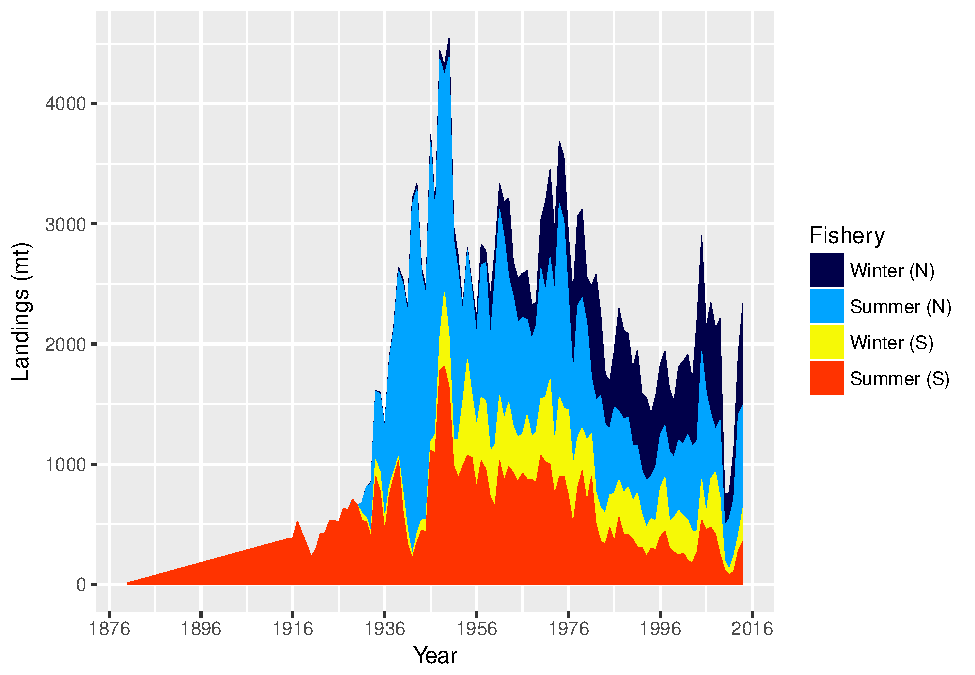
\includegraphics{Petrale_2019_Update_files/figure-latex/unnamed-chunk-13-1.pdf}
\caption{Landings of Petrale sole by the Northern and Southern winter
and summer fleets of the US west coast. \label{fig:Exec_catch1}}
\end{figure}

\FloatBarrier

\subsection*{Data and Assessment}\label{data-and-assessment}
\addcontentsline{toc}{subsection}{Data and Assessment}

This an update assessment for Petrale sole, which was last assessed in
2013 and updated in 2015. The update assessment was conducted using the
length- and age-structured modeling software Stock Synthesis (version
3.30.03.XX). The coastwide population was modeled allowing separate
growth and mortality parameters for each sex (a two-sex model) with the
fishing year beginning on November 1 and ending on October 31. The
fisheries are structured seasonally based on winter (November to
February) and summer (March to October) fishing seasons due to the
development and growth of the wintertime fishery, which began in the
1950s. In recent decades wintertime catches have often exceed summertime
catches. The fisheries modeled as the North Winter and North Summer,
where the north includes both Washington and Oregon, and South Winter
and South Summer encompasses California fisheries.

The model includes catch, length- and age-frequency data from the trawl
fleets as well as standardized winter fishery catch-per-unit-effort
(CPUE) indices. Biological data are derived from both port and on-board
observer sampling programs. The National Marine Fisheries Service (NMFS)
early (1980, 1983, 1986, 1989, 1992) and late (1995, 1998, 2001, and
2004) Triennial bottom trawl survey and the Northwest Fisheries Science
Center (NWFSC) trawl survey (2003-2018) relative biomass indices and
biological sampling provide fishery independent information on relative
trend and demographics of the Petrale sole stock.

\subsection*{Updated Data}\label{updated-data}
\addcontentsline{toc}{subsection}{Updated Data}

The base stock assessment model structure is consistent with the 2013
assessment and the 2015 update, except as noted here. Additions to the
model include 1) landings data for 2015 - 2018, 2) commercial
composition data (age and length) for 2015 - 2018, 3) NWFSC groundfish
trawl survey index for 2015 - 2018, and 4) age and length composition
data from the NWFSC groundfish trawl survey.

Modifications from the previous assessment model include:

\begin{enumerate}

\item Survey indices were calculated using VAST.

\item Length-weight relationship parameters estimated outside of the stock assessment model from the NWFSC groundfish trawl survey data up to 2018 and input as fixed values.

\item Early commercial age data for OR and WA were not combined, consistent with the 2011 assessment.

\item Fitting using SS v.3.30.XX. 

\item Model tuning to re-weight data. 

\end{enumerate}

\subsection*{Stock Biomass}\label{stock-biomass}
\addcontentsline{toc}{subsection}{Stock Biomass}

The predicted spawning output from the base model \ldots{}

\begin{figure}
\centering
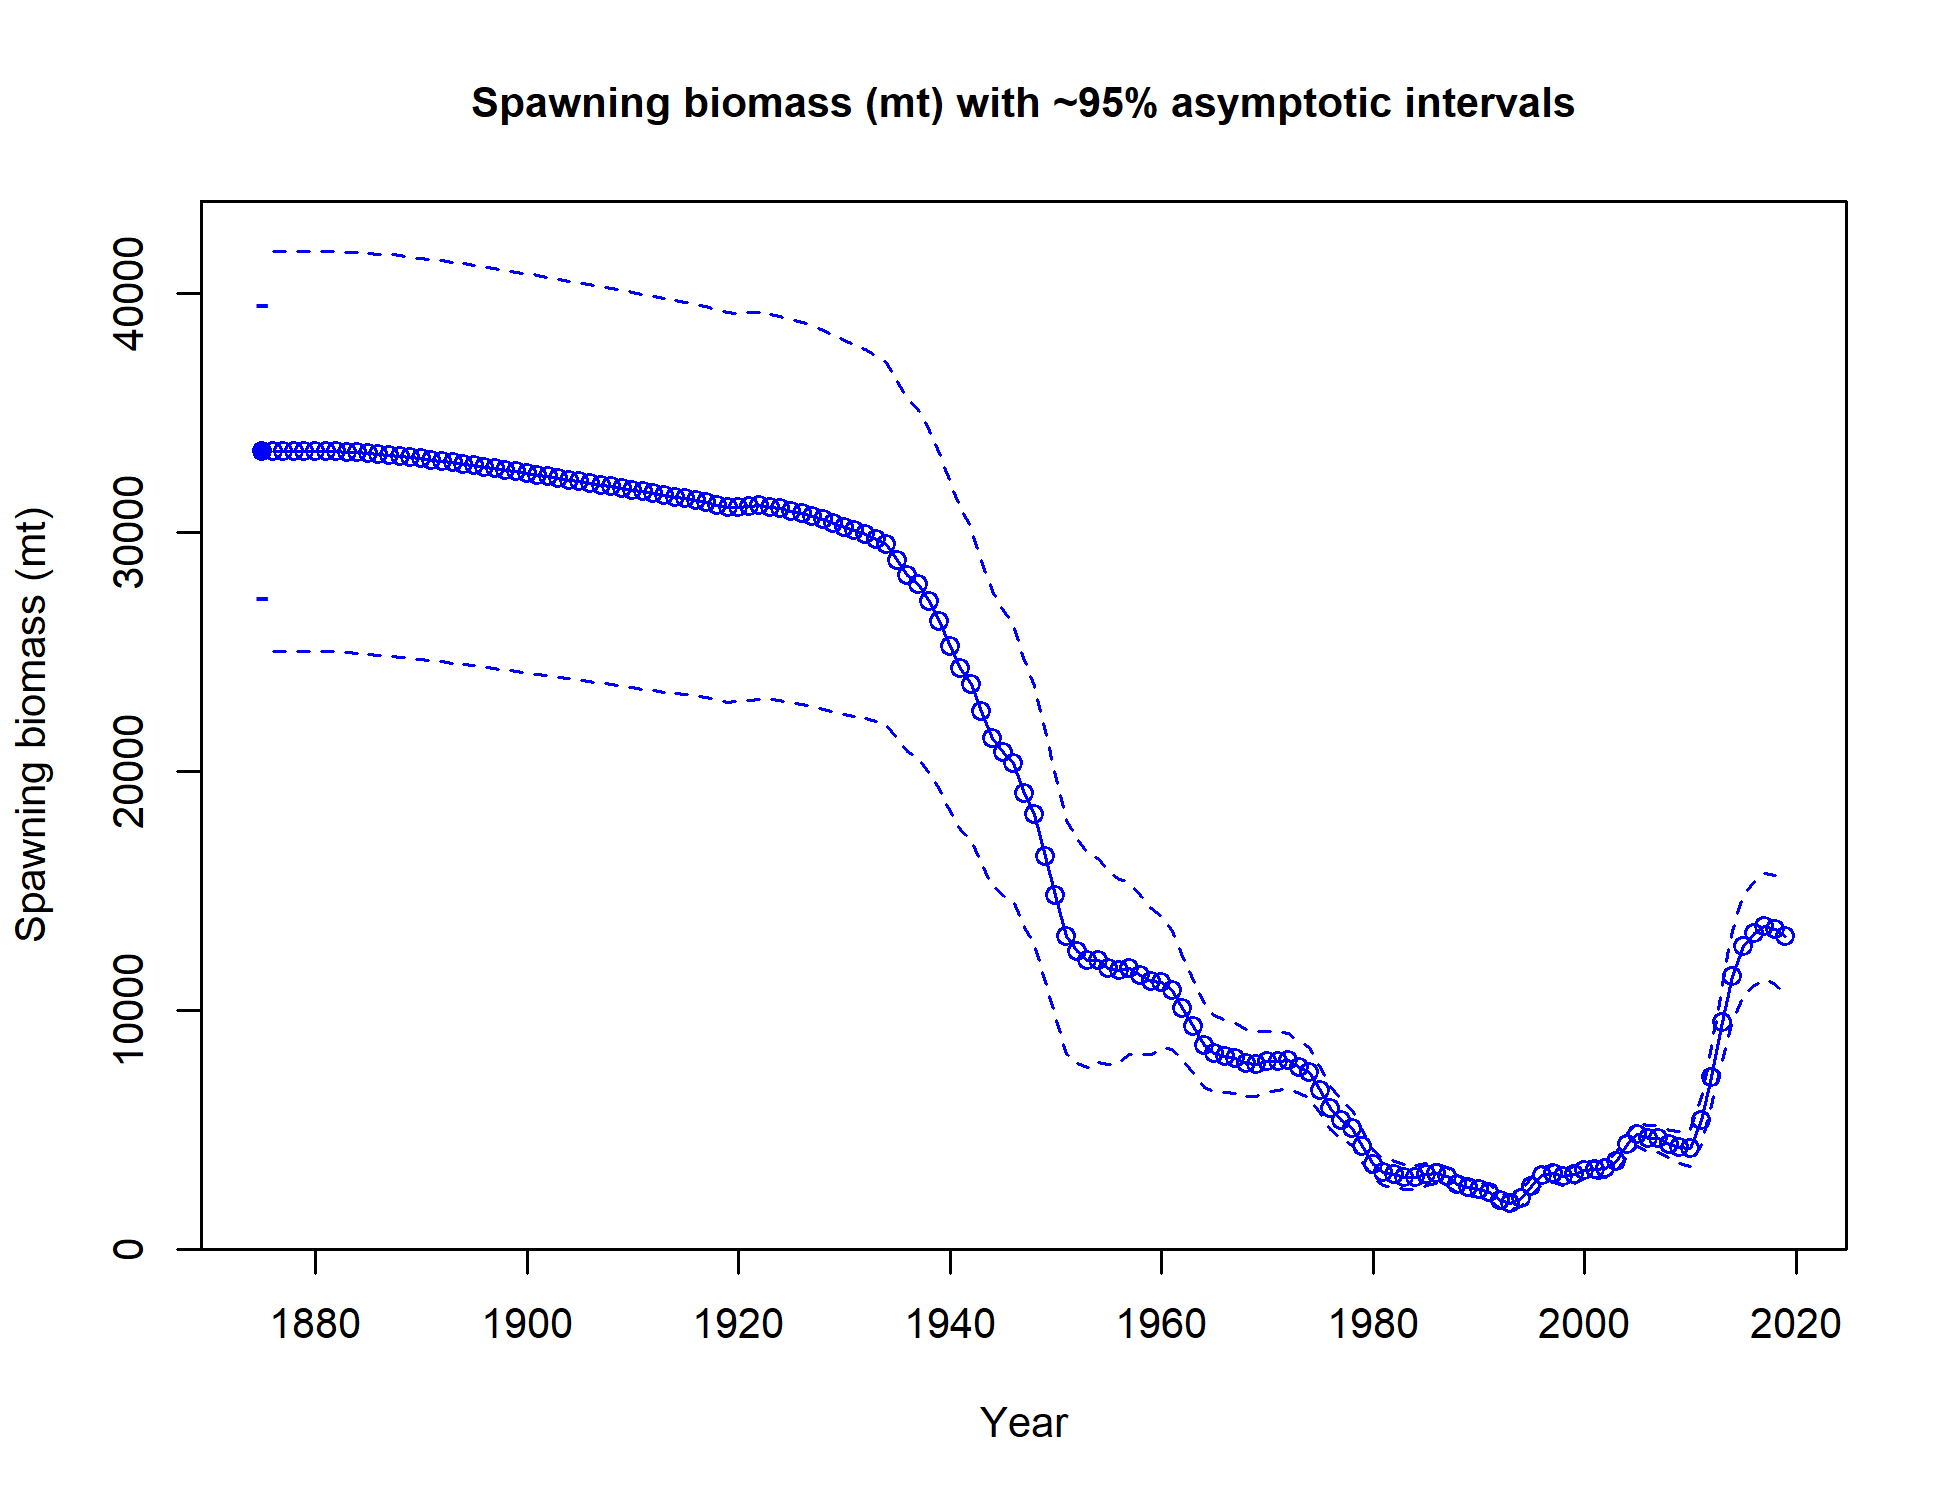
\includegraphics{r4ss/plots_mod1/ts7_Spawning_biomass_(mt)_with_95_asymptotic_intervals_intervals.png}
\caption{Estimated time-series of spawning output trajectory (circles
and line: median; light broken lines: 95\% credibility intervals) for
the base assessment model. \label{fig:Spawnbio_all}}
\end{figure}

\begin{figure}
\centering
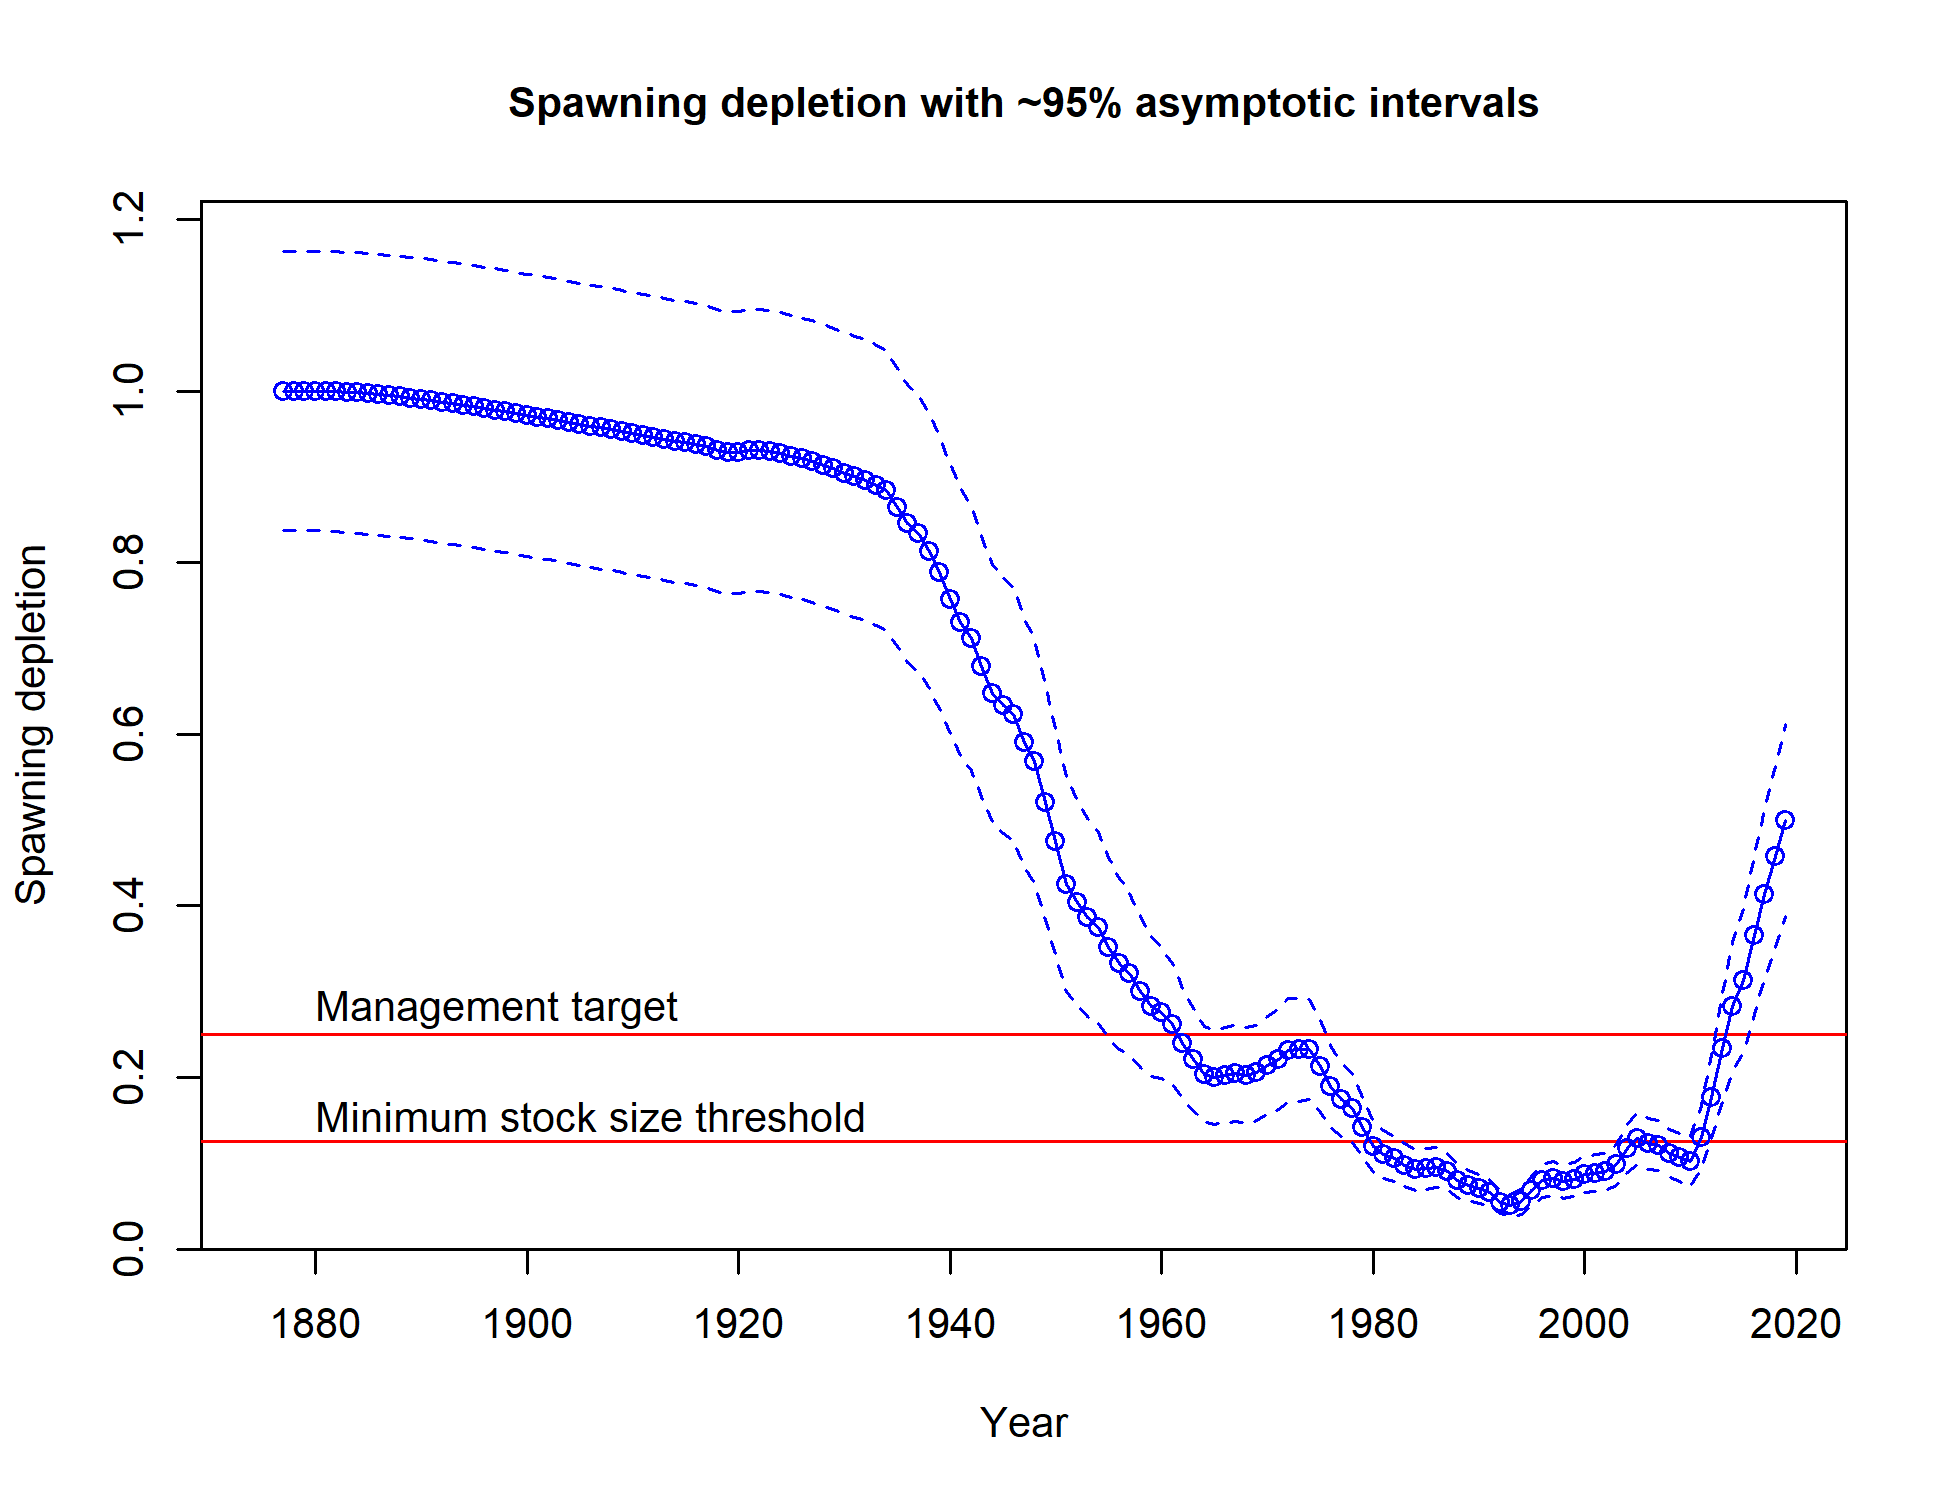
\includegraphics{r4ss/plots_mod1/ts9_Spawning_depletion_with_95_asymptotic_intervals_intervals.png}
\caption{Estimated time-series of relative spawning output (depletion)
(circles and line: median; light broken lines: 95\% credibility
intervals) for the base assessment model. \label{fig:RelDeplete_all}}
\end{figure}

\begin{table}[ht]
\centering
\caption{Recent trend in estimated spawning output (mt) and estimated relative spawning output (depletion).} 
\label{tab:SpawningDeplete_mod1}
\begin{tabular}{l>{\centering}p{1.3in}>{\centering}p{1.2in}>{\centering}p{1in}>{\centering}p{1.2in}}
  \hline
Year & Spawning Output (mt) & \~{} 95\% Confidence Interval & Estimated Depletion & \~{} 95\% Confidence Interval \\ 
  \hline
2010 & 3448 & 2895 - 4001 & 0.102 & 0.073 - 0.131 \\ 
  2011 & 4396 & 3691 - 5101 & 0.130 & 0.094 - 0.167 \\ 
  2012 & 5957 & 5020 - 6895 & 0.177 & 0.128 - 0.225 \\ 
  2013 & 7887 & 6641 - 9133 & 0.234 & 0.171 - 0.297 \\ 
  2014 & 9514 & 7942 - 11086 & 0.282 & 0.207 - 0.358 \\ 
  2015 & 10531 & 8672 - 12390 & 0.313 & 0.229 - 0.396 \\ 
  2016 & 12329 & 10225 - 14433 & 0.366 & 0.273 - 0.458 \\ 
  2017 & 13910 & 11567 - 16254 & 0.413 & 0.314 - 0.512 \\ 
  2018 & 15401 & 12797 - 18005 & 0.457 & 0.352 - 0.562 \\ 
  2019 & 16841 & 13924 - 19758 & 0.500 & 0.388 - 0.612 \\ 
   \hline
\end{tabular}
\end{table}

\FloatBarrier

\subsection*{Recruitment}\label{recruitment}
\addcontentsline{toc}{subsection}{Recruitment}

Recruitment deviations were estimated for the entire assessment
period\ldots{}

\begin{figure}
\centering
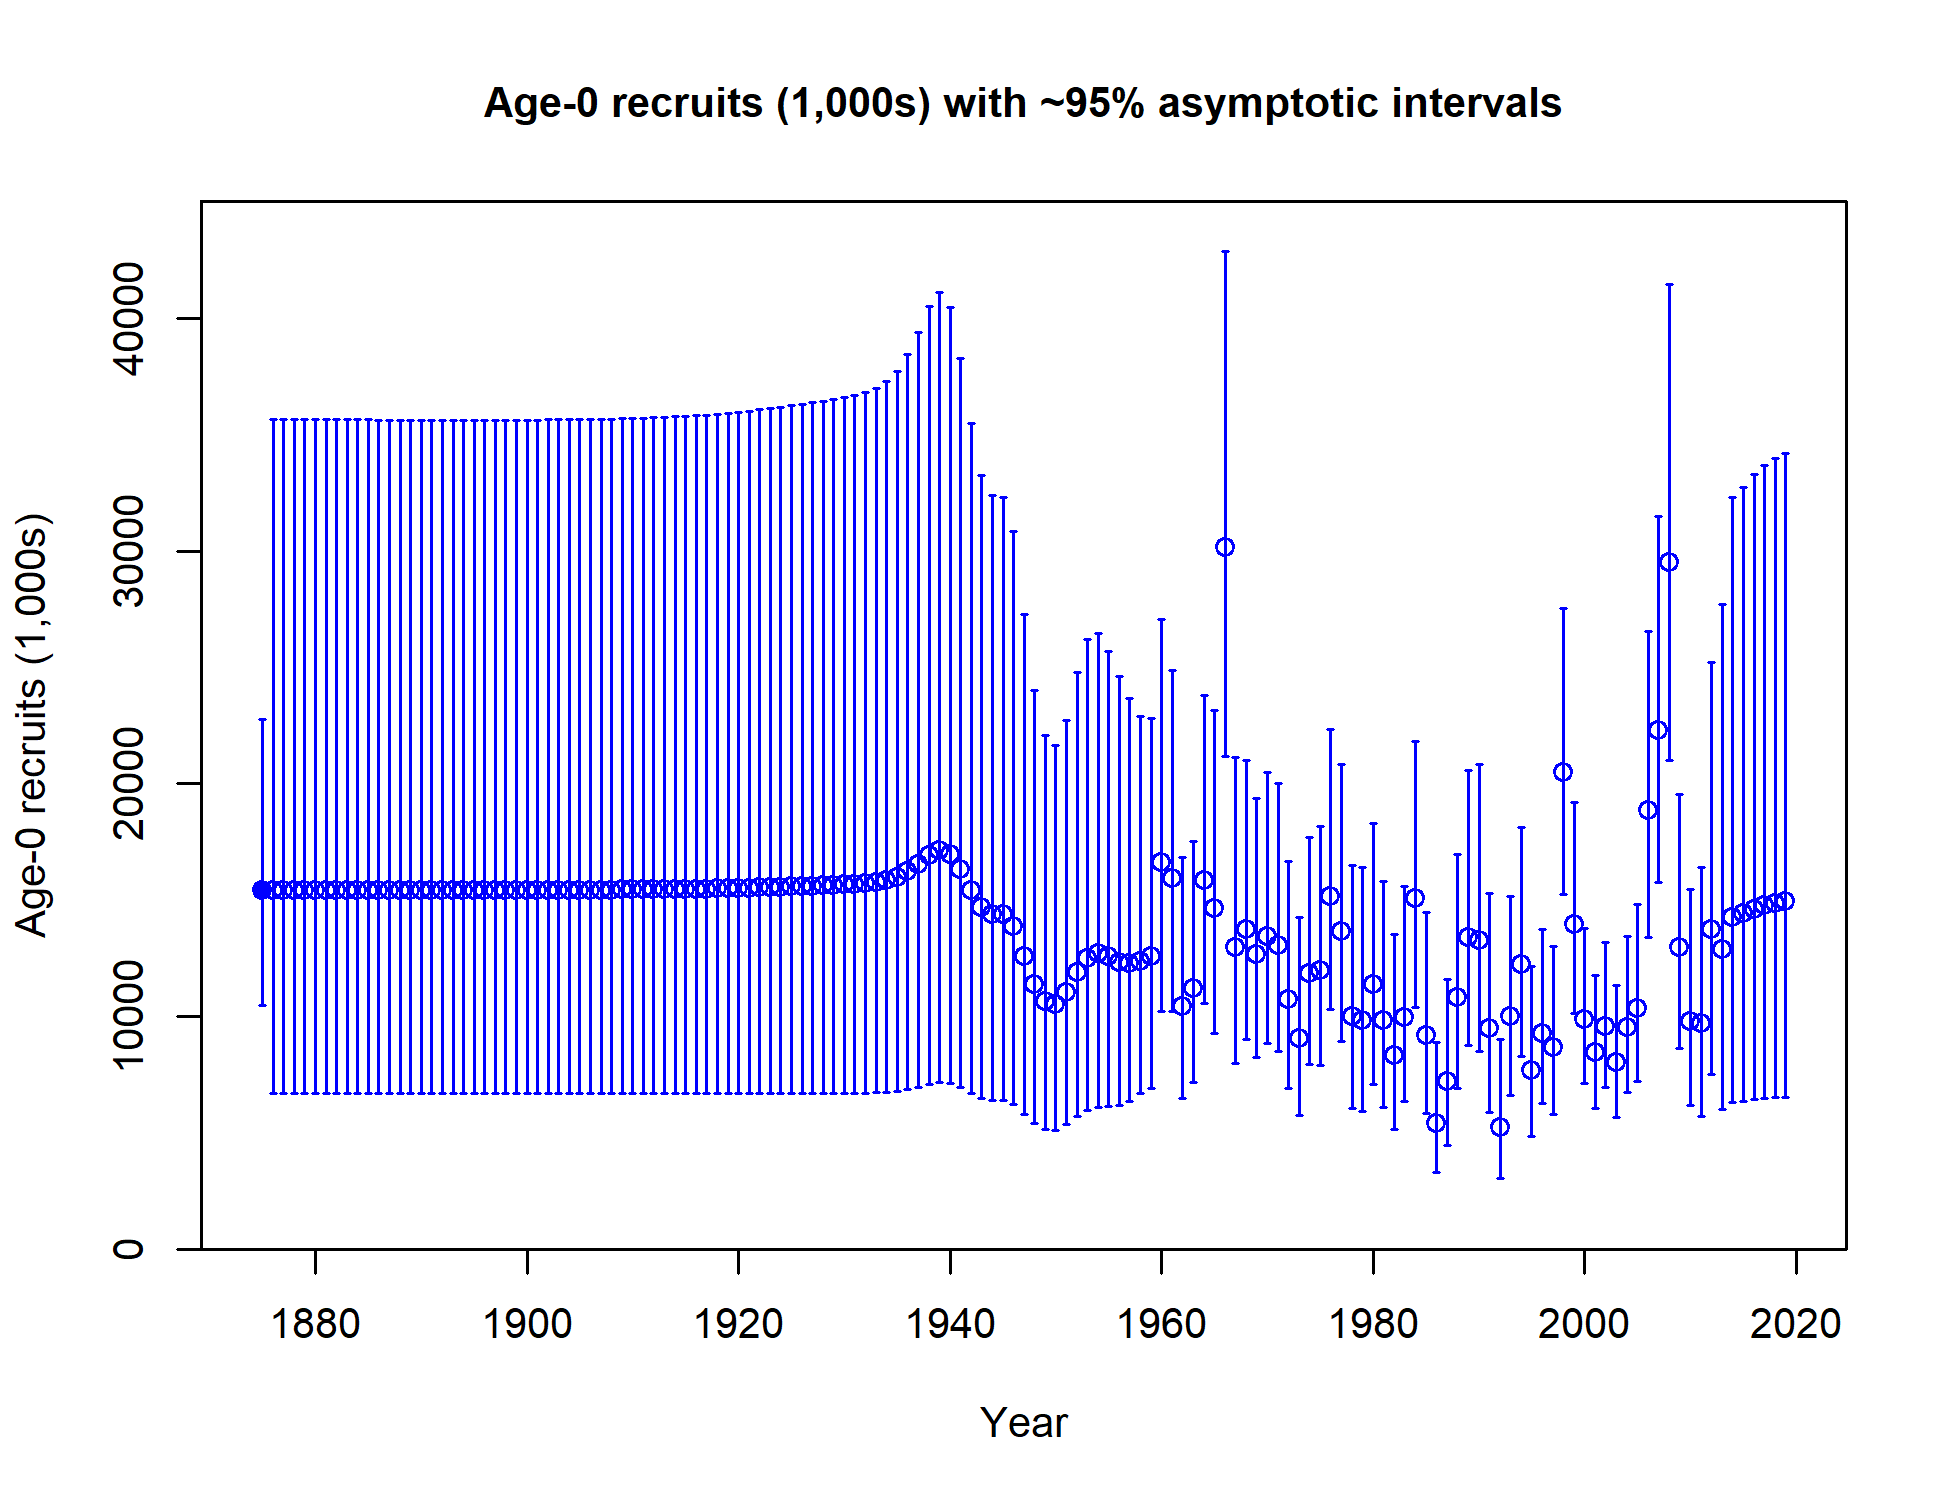
\includegraphics{r4ss/plots_mod1/ts11_Age-0_recruits_(1000s)_with_95_asymptotic_intervals.png}
\caption{Time-series of estimated Petrale sole recruitments for the base
model with 95\% confidence or credibility intervals.
\label{fig:Recruits_all}}
\end{figure}

\begin{table}[ht]
\centering
\caption{Recent estimated trend in recruitment and estimated recruitment deviations determined from the base model. The recruitment deviations for 2016 and 2017 were fixed at zero within the model.} 
\label{tab:Recruit_mod1}
\begin{tabular}{>{\centering}p{.8in}>{\centering}p{1.0in}>{\centering}p{1.4in}>{\centering}p{1.0in}>{\centering}p{1.4in}}
  \hline
Year & Estimated Recruitment & \~{} 95\% Confidence Interval & Estimated Recruitment Devs. & \~{} 95\% Confidence Interval \\ 
  \hline
2010 & 9787 & 6190 - 15473 & -0.144 & -0.509 - 0.220 \\ 
  2011 & 9683 & 5721 - 16387 & -0.209 & -0.654 - 0.236 \\ 
  2012 & 13760 & 7506 - 25228 & 0.067 & -0.467 - 0.601 \\ 
  2013 & 12874 & 5985 - 27695 & -0.060 & -0.789 - 0.668 \\ 
  2014 & 14272 & 6300 - 32334 & -0.000 & -0.784 - 0.784 \\ 
  2015 & 14418 & 6351 - 32730 & 0.000 & -0.784 - 0.784 \\ 
  2016 & 14621 & 6422 - 33289 & 0.000 & -0.784 - 0.784 \\ 
  2017 & 14760 & 6470 - 33673 & 0.000 & -0.784 - 0.784 \\ 
  2018 & 14867 & 6506 - 33972 & 0.000 & -0.784 - 0.784 \\ 
  2019 & 14953 & 6534 - 34219 & 0.000 & -0.784 - 0.784 \\ 
   \hline
\end{tabular}
\end{table}

\FloatBarrier

\subsection*{Exploitation Status}\label{exploitation-status}
\addcontentsline{toc}{subsection}{Exploitation Status}

The spawning output of Petrale sole\ldots{}

\begin{table}[ht]
\centering
\caption{Recent trend in spawning potential ratio (1-SPR)/(1-SPR50) and summary exploitation rate for age 3+ biomass for Petrale sole.} 
\label{tab:SPR_Exploit_mod1}
\begin{tabular}{l>{\centering}p{0.9in}>{\centering}p{1.2in}>{\centering}p{1.2in}>{\centering}p{1.2in}}
  \hline
Year & (1-SPR)/ (1-SPR50\%) & \~{} 95\% Confidence Interval & Exploitation Rate & \~{} 95\% Confidence Interval \\ 
  \hline
2009 & 0.847 & 0.793 - 0.900 & 0.278 & 0.236 - 0.319 \\ 
  2010 & 0.672 & 0.583 - 0.762 & 0.099 & 0.080 - 0.117 \\ 
  2011 & 0.581 & 0.487 - 0.674 & 0.063 & 0.052 - 0.074 \\ 
  2012 & 0.592 & 0.503 - 0.682 & 0.074 & 0.061 - 0.086 \\ 
  2013 & 0.656 & 0.572 - 0.739 & 0.110 & 0.092 - 0.128 \\ 
  2014 & 0.654 & 0.571 - 0.736 & 0.124 & 0.103 - 0.145 \\ 
  2015 & 0.006 & 0.004 - 0.008 & 0.001 & 0.000 - 0.001 \\ 
  2016 & 0.005 & 0.004 - 0.007 & 0.000 & 0.000 - 0.001 \\ 
  2017 & 0.005 & 0.003 - 0.006 & 0.000 & 0.000 - 0.000 \\ 
  2018 & 0.004 & 0.003 - 0.005 & 0.000 & 0.000 - 0.000 \\ 
   \hline
\end{tabular}
\end{table}

\FloatBarrier

\begin{figure}
\centering
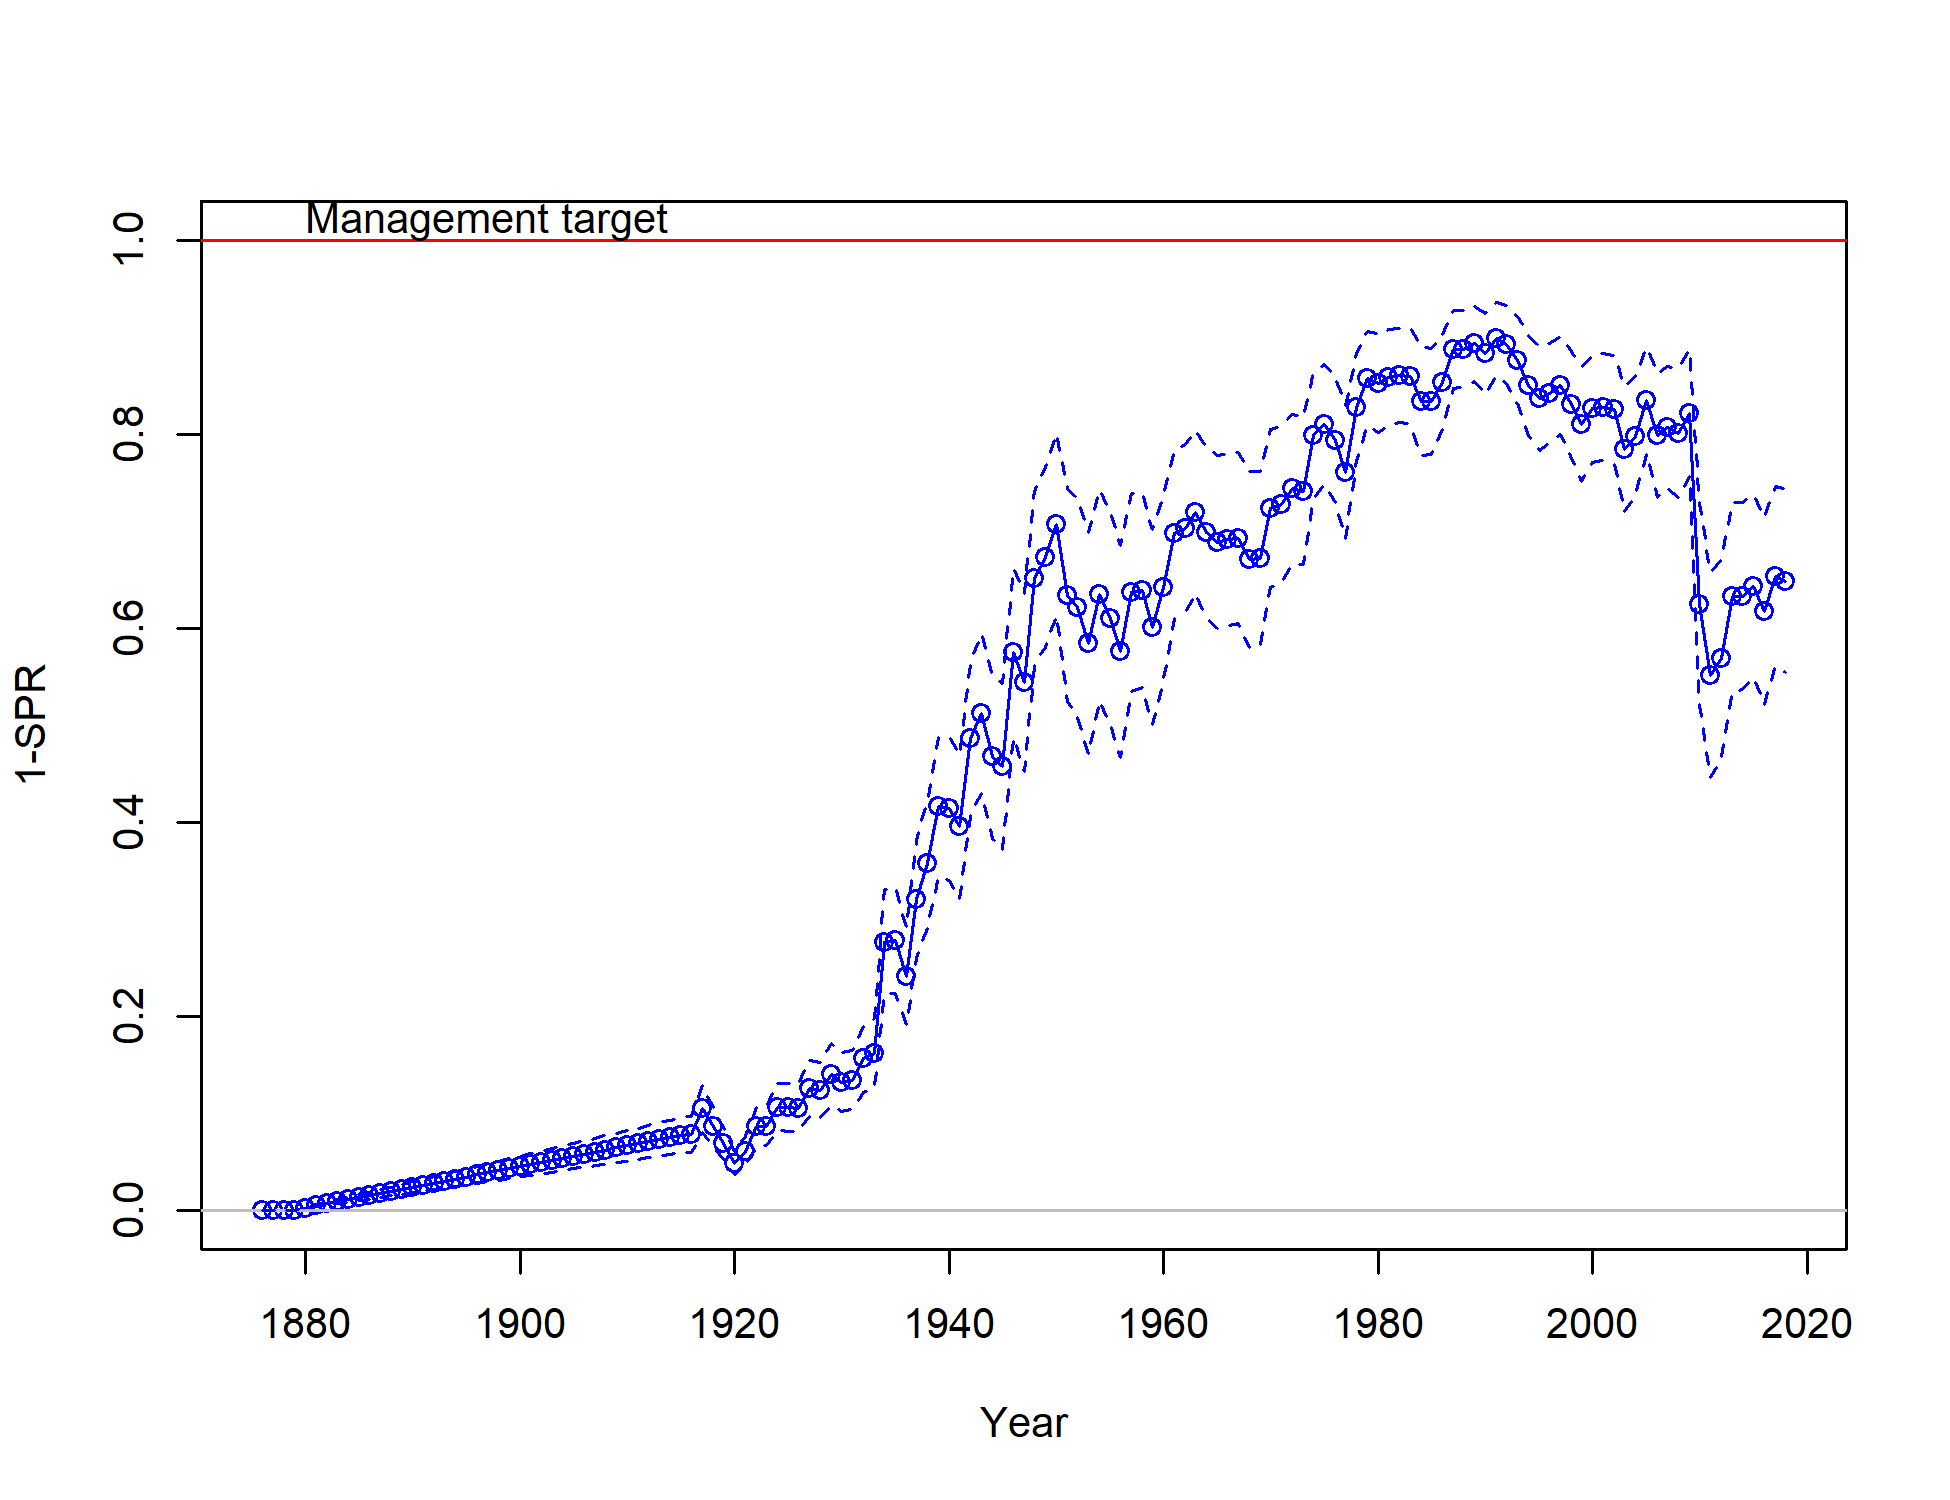
\includegraphics{r4ss/plots_mod1/SPR3_ratiointerval.png}
\caption{Estimated relative spawning potential ratio (1-SPR)/(1-SPR30\%)
for the base model. One minus SPR is plotted so that higher exploitation
rates occur on the upper portion of the y-axis. The management target is
plotted as a red horizontal line and values above this reflect harvests
in excess of the overfishing proxy based on the SPR30\% harvest rate.
The last year in the time-series is 2018. \label{fig:SPR_all}}
\end{figure}

\begin{figure}
\centering
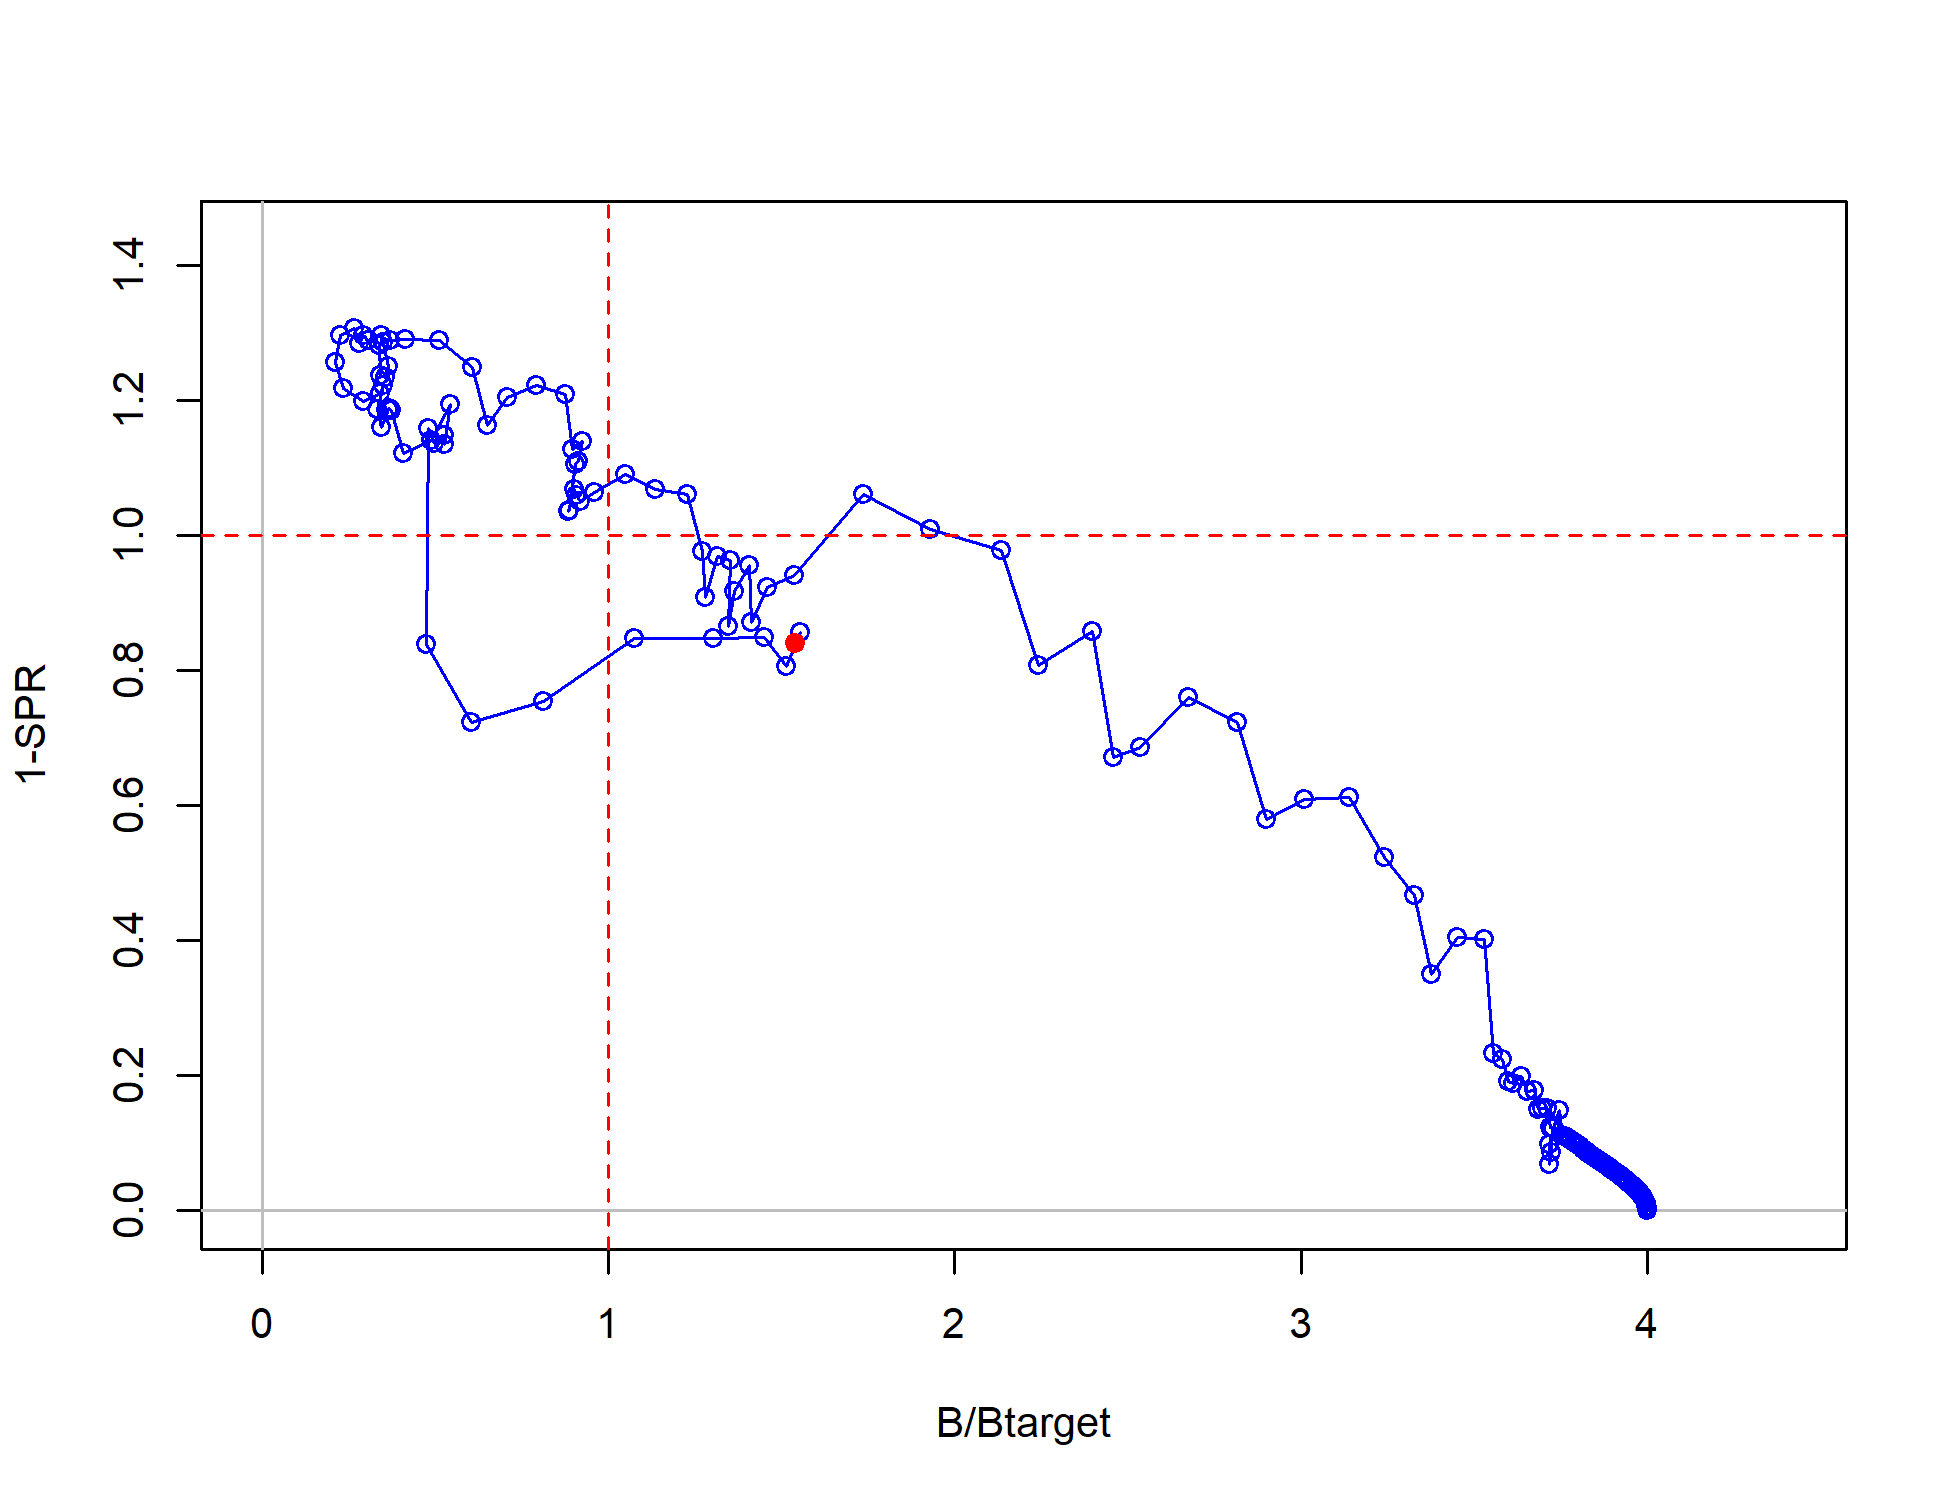
\includegraphics{r4ss/plots_mod1/SPR4_phase.png}
\caption{Phase plot of estimated (1-SPR)/(1-SPR30\%) vs.~depletion
(B/Btarget) for the base case model. The red circle indicates 2018
estimated status and exploitation for Petrale sole.
\label{fig:Phase_all}}
\end{figure}

\FloatBarrier

\subsection*{Ecosystem Considerations}\label{ecosystem-considerations}
\addcontentsline{toc}{subsection}{Ecosystem Considerations}

\subsection*{Reference Points}\label{reference-points}
\addcontentsline{toc}{subsection}{Reference Points}

This stock assessment estimates that the spawning output of Petrale sole
is above the management target. Due to reduced landing and the large
2008 year-class, an increasing trend in spawning output was estimated in
the base model. The estimated depletion in 2019 is 50.0\% (\(\sim\) 95\%
asymptotic interval: \(\pm\) 38.8\%-61.2\%), corresponding to an
unfished spawning output of 16,841 mt (\(\sim\) 95\% asymptotic
interval: 13,924-19,758 mt). Unfished age 3+ biomass was estimated to be
53,873.7 mt in the base model. The target spawning output based on the
biomass target (\(SB_{25\%}\)) is 8,423.3 mt, with an equilibrium catch
of 2,729.5 mt. Equilibrium yield at the proxy \(F_{MSY}\) harvest rate
corresponding to \(SPR_{30\%}\) is 2,702.4 mt. Estimated MSY catch is at
a 2,742.2 spawning output of 7,323.1 mt (21.7\% depletion)

\begin{table}[ht]
\centering
\caption{Summary of reference 
                                      points and management quantities for the 
                                      base case.} 
\label{tab:Ref_pts_mod1}
\begin{tabular}{>{\raggedright}p{4.1in}>{\centering}p{.65in}>{\centering}p{.65in}>{\centering}p{.65in}}
  \hline
\textbf{Quantity} & \textbf{Estimate} & \textbf{$\sim$2.5\%  Confidence Interval} & \textbf{$\sim$97.5\%  Confidence Interval} \\ 
  \hline
Unfished spawning output (mt) & 33693.4 & 27542.4 & 39844.4 \\ 
  Unfished age 3+ biomass (mt) & 53873.7 & 45675.1 & 62072.3 \\ 
  Unfished recruitment (R0, thousands) & 15430.6 & 9369.1 & 21492.1 \\ 
  Spawning output(2019 mt) & 16841.1 & 13924 & 19758.2 \\ 
  Relative spawning output (depletion) (2019) & 0.5 & 0.388 & 0.612 \\ 
  \textbf{$\text{Reference points based on } \mathbf{SB_{25\%}}$} &  &  &  \\ 
  Proxy spawning output ($B_{25\%}$) & 8423.3 & 6885.6 & 9961.1 \\ 
  SPR resulting in $B_{25\%}$ ($SPR_{B25\%}$) & 0.274 & 0.251 & 0.297 \\ 
  Exploitation rate resulting in $B_{25\%}$ & 0.166 & 0.147 & 0.186 \\ 
  Yield with $SPR_{B25\%}$ at $B_{25\%}$ (mt) & 2729.5 & 2472.1 & 2986.8 \\ 
  \textbf{\textit{Reference points based on SPR proxy for MSY}} &  &  &  \\ 
  Spawning output & 9329.8 & 7316.9 & 11342.7 \\ 
  $SPR_{30\%}$ &  &  &  \\ 
  Exploitation rate corresponding to $SPR_{30\%}$ & 0.151 & 0.125 & 0.178 \\ 
  Yield with $SPR_{30\%}$ at $SB_{SPR}$ (mt) & 2702.4 & 2414.6 & 2990.2 \\ 
  \textbf{\textit{Reference points based on estimated MSY values}} &  &  &  \\ 
  Spawning output at $MSY$ ($SB_{MSY}$) & 7323.1 & 5504.8 & 9141.4 \\ 
  $SPR_{MSY}$ & 0.242 & 0.18 & 0.304 \\ 
  Exploitation rate at $MSY$ & 0.187 & 0.157 & 0.216 \\ 
  $MSY$ (mt)  & 2742.2 & 2502.5 & 2982 \\ 
   \hline
\end{tabular}
\end{table}

\FloatBarrier

\subsection*{Management Performance}\label{management-performance}
\addcontentsline{toc}{subsection}{Management Performance}

Exploitation rates on Petrale sole\ldots{}

\begin{table}[ht]
\centering
\caption{Recent trend in total catch and  
                              landings (mt) relative to the management guidelines. 
                              Estimated total catch reflect the landings 
                              plus the model estimated discarded biomass based on discard rate data.} 
\label{tab:mnmgt_perform}
\scalebox{0.9}{
\begin{tabular}{>{\raggedleft}p{0.5in}>{\centering}p{1.1in}>{\centering}p{1.1in}>{\centering}p{1.1in}>{\centering}p{1.1in}}
  \hline
Year & OFL (mt; ABC prior to 2011) & ACL (mt; OY prior to 2011) & Total Landings (mt) & Estimated Total Catch (mt) \\ 
  \hline
\text{2009} & 2,811 & 2433 & 2208 & 2323 \\ 
  \text{2010} & 2,751 & 1200 & 749 & 914 \\ 
  \text{2011} & 1,021 & 976 & 762 & 781 \\ 
  \text{2012} & 1,275 & 1160 & 1116 & 1135 \\ 
  \text{2013} & 2,711 & 2592 & 1925 & 1954 \\ 
  \text{2014} & 2,774 & 2652 & 2341 & 2361 \\ 
  \text{2015} & 3,073 & 2816 & 10 & 10 \\ 
  \text{2016} & 3,208 & 2910 & 10 & 10 \\ 
  \text{2017} & 3,208 & 3,136 & 10 & 10 \\ 
  \text{2018} & 3,152 & 3,013 & 10 & 10 \\ 
   \hline
\end{tabular}
}
\end{table}

\FloatBarrier

\subsection*{Unresolved Problems and Major
Uncertainties}\label{unresolved-problems-and-major-uncertainties}
\addcontentsline{toc}{subsection}{Unresolved Problems and Major
Uncertainties}

\begin{enumerate}

\item The current data for Petrale sole weighted according to the Francis weighting...  


\end{enumerate}

\subsection*{Decision Table}\label{decision-table}
\addcontentsline{toc}{subsection}{Decision Table}

Model uncertainty has been described by the estimated uncertainty within
the base model and by the sensitivities to different model structure.

\begin{table}[ht]
\centering
\caption{Projections of potential OFL (mt) and ABC (mt) and the estimated spawning output and relative depletion based on ABC removals.  The 2019 and 2020 
                                               removals are set at the harvest limits currently set by management of XXX mt per year.} 
\label{tab:OFL_projection}
\begin{tabular}{>{\raggedleft}p{0.5in}>{\centering}p{1.1in}>{\centering}p{1.1in}>{\centering}p{1.6in}>{\centering}p{1.1in}}
  \hline
Year & OFL & ABC & Spawning Output (mt) & Relative Depletion \\ 
  \hline
2019 & 4834 & 4640 & 16841 & 0.500 \\ 
  2020 & 4396 & 4219 & 15401 & 0.457 \\ 
  2021 & 4036 & 3873 & 14183 & 0.421 \\ 
  2022 & 3750 & 3599 & 13192 & 0.392 \\ 
  2023 & 3532 & 3389 & 12412 & 0.368 \\ 
  2024 & 3367 & 3231 & 11814 & 0.351 \\ 
  2025 & 3244 & 3113 & 11362 & 0.337 \\ 
  2026 & 3152 & 3025 & 11020 & 0.327 \\ 
  2027 & 3082 & 2958 & 10758 & 0.319 \\ 
  2028 & 3028 & 2906 & 10554 & 0.313 \\ 
  2029 & 2986 & 2865 & 10394 & 0.308 \\ 
  2030 & 2952 & 2832 & 10266 & 0.305 \\ 
   \hline
\end{tabular}
\end{table}

\FloatBarrier

\begin{table}[ht]
\centering
\caption{Decision table summary of 10-year 
                                             projections beginning in 2021 
                                             for alternate states of nature based on 
                                             an axis of uncertainty for the base model. The removals in 2019 and 2020 were set at the defined management 
                                             specification of XXX mt for each year assuming full attainment.
                                             The range of natural mortality values corresponded to the 12.5 and 87.5th quantile
                                             from the uncertainty around final spawning biomass.
                                             Columns range over low, mid, and high
                                             states of nature, and rows range over different 
                                             assumptions of catch levels. The SPR50 catch stream is based on the equilibrium yield applying the SPR50 harvest rate.} 
\label{tab:Decision_table_mod1}
\scalebox{0.85}{
\begin{tabular}{l|cc|>{\centering}p{.7in}c|>{\centering}p{.7in}c|>{\centering}p{.7in}c}
   \multicolumn{3}{c}{}  &  \multicolumn{2}{c}{} 
                               & \multicolumn{2}{c}{\textbf{States of nature}} 
                               & \multicolumn{2}{c}{} \\
  \multicolumn{3}{c}{}  &  \multicolumn{2}{c}{M = 0.04725} 
                               & \multicolumn{2}{c}{M = 0.054} 
                               &  \multicolumn{2}{c}{M = 0.0595} \\
 \hline
 & Year & Catch & Spawning Output & Depletion (\%) & Spawning Output & Depletion (\%) & Spawning Output & Depletion (\%) \\ 
  \hline
 & 2021 &  &  &  &  &  &  &  \\ 
   & 2022 &  &  &  &  &  &  &  \\ 
   & 2023 &  &  &  &  &  &  &  \\ 
  ABC & 2024 &  &  &  &  &  &  &  \\ 
   & 2025 &  &  &  &  &  &  &  \\ 
   & 2026 &  &  &  &  &  &  &  \\ 
   & 2027 &  &  &  &  &  &  &  \\ 
   & 2028 &  &  &  &  &  &  &  \\ 
   & 2029 &  &  &  &  &  &  &  \\ 
   & 2030 &  &  &  &  &  &  &  \\ 
   \hline
 & 2021 &  &  &  &  &  &  &  \\ 
   & 2022 &  &  &  &  &  &  &  \\ 
   & 2023 &  &  &  &  &  &  &  \\ 
  SPR target = 0.34 & 2024 &  &  &  &  &  &  &  \\ 
   & 2025 &  &  &  &  &  &  &  \\ 
   & 2026 &  &  &  &  &  &  &  \\ 
   & 2027 &  &  &  &  &  &  &  \\ 
   & 2028 &  &  &  &  &  &  &  \\ 
   & 2029 &  &  &  &  &  &  &  \\ 
   & 2030 &  &  &  &  &  &  &  \\ 
   \hline
\end{tabular}
}
\end{table}

\FloatBarrier

\subsection*{Research and Data Needs}\label{research-and-data-needs}
\addcontentsline{toc}{subsection}{Research and Data Needs}

There are many areas of research that could be undertaken to benefit the
understanding and assessment of Petrale sole. Below, are issues that are
considered of importance.

\begin{enumerate}

\item \textbf{Natural mortality}: 

\item \textbf{Steepness}: 

\item \textbf{Basin-wide understanding of stock structure, biology, connectivity, and distribution:} 

\end{enumerate}

\begin{sidewaystable}[ht]
\centering
\caption{Base model results summary.} 
\label{tab:base_summary}
\scalebox{0.6}{
\begin{tabular}{r>{\centering}p{1.1in}>{\centering}p{1.1in}>{\centering}p{1.1in}>{\centering}p{1.1in}>{\centering}p{1.1in}>{\centering}p{1.1in}>{\centering}p{1.1in}>{\centering}p{1.1in}>{\centering}p{1.1in}>{\centering}p{1.1in}}
  \hline
Quantity & 2010 & 2011 & 2012 & 2013 & 2014 & 2015 & 2016 & 2017 & 2018 & 2019 \\ 
  \hline
OFL (mt) & 2,751 & 1,021 & 1,275 & 2,711 & 2,774 & 3,073 & 3,208 & 3,208 & 3,152 & 1 \\ 
  ACL (mt) & 1200 & 976 & 1160 & 2592 & 2652 & 2816 & 2910 & 3,136 & 3,013 & 1 \\ 
  Landings (mt) &  749 &  762 & 1116 & 1925 & 2341 &   10 &   10 &   10 &   10 &  \\ 
  Total Est. Catch (mt) &  914 &  781 & 1135 & 1954 & 2361 &   10 &   10 &   10 &   10 &  \\ 
   \hline
(1-$SPR$)(1-$SPR_{50\%}$) & 0.672 & 0.581 & 0.592 & 0.656 & 0.654 & 0.006 & 0.005 & 0.005 & 0.004 &  \\ 
   \hline
Exploitation rate & 0.099 & 0.063 & 0.074 & 0.110 & 0.124 & 0.001 & 0.000 & 0.000 & 0.000 &  \\ 
  Age 3+ biomass (mt) &  9271.69 & 12406.50 & 15359.80 & 17730.40 & 18994.80 & 19707.20 & 22306.10 & 24807.50 & 27178.10 & 29422.30 \\ 
   \hline
Spawning Output &  3448 &  4396 &  5957 &  7887 &  9514 & 10531 & 12329 & 13910 & 15401 & 16841 \\ 
  ~95\% CI & 2895 - 4001 & 3691 - 5101 & 5020 - 6895 & 6641 - 9133 & 7942 - 11086 & 8672 - 12390 & 10225 - 14433 & 11567 - 16254 & 12797 - 18005 & 13924 - 19758 \\ 
   \hline
Relative Depletion & 0.102 & 0.130 & 0.177 & 0.234 & 0.282 & 0.313 & 0.366 & 0.413 & 0.457 & 0.500 \\ 
  ~95\% CI & 0.073 - 0.131 & 0.094 - 0.167 & 0.128 - 0.225 & 0.171 - 0.297 & 0.207 - 0.358 & 0.229 - 0.396 & 0.273 - 0.458 & 0.314 - 0.512 & 0.352 - 0.562 & 0.388 - 0.612 \\ 
   \hline
Recruits &  9787 &  9683 & 13760 & 12874 & 14272 & 14418 & 14621 & 14760 & 14867 & 14953 \\ 
  ~95\% CI & 6190 - 15473 & 5721 - 16387 & 7506 - 25228 & 5985 - 27695 & 6300 - 32334 & 6351 - 32730 & 6422 - 33289 & 6470 - 33673 & 6506 - 33972 & 6534 - 34219 \\ 
   \hline
\end{tabular}
}
\end{sidewaystable}

\FloatBarrier

\begin{figure}
\centering
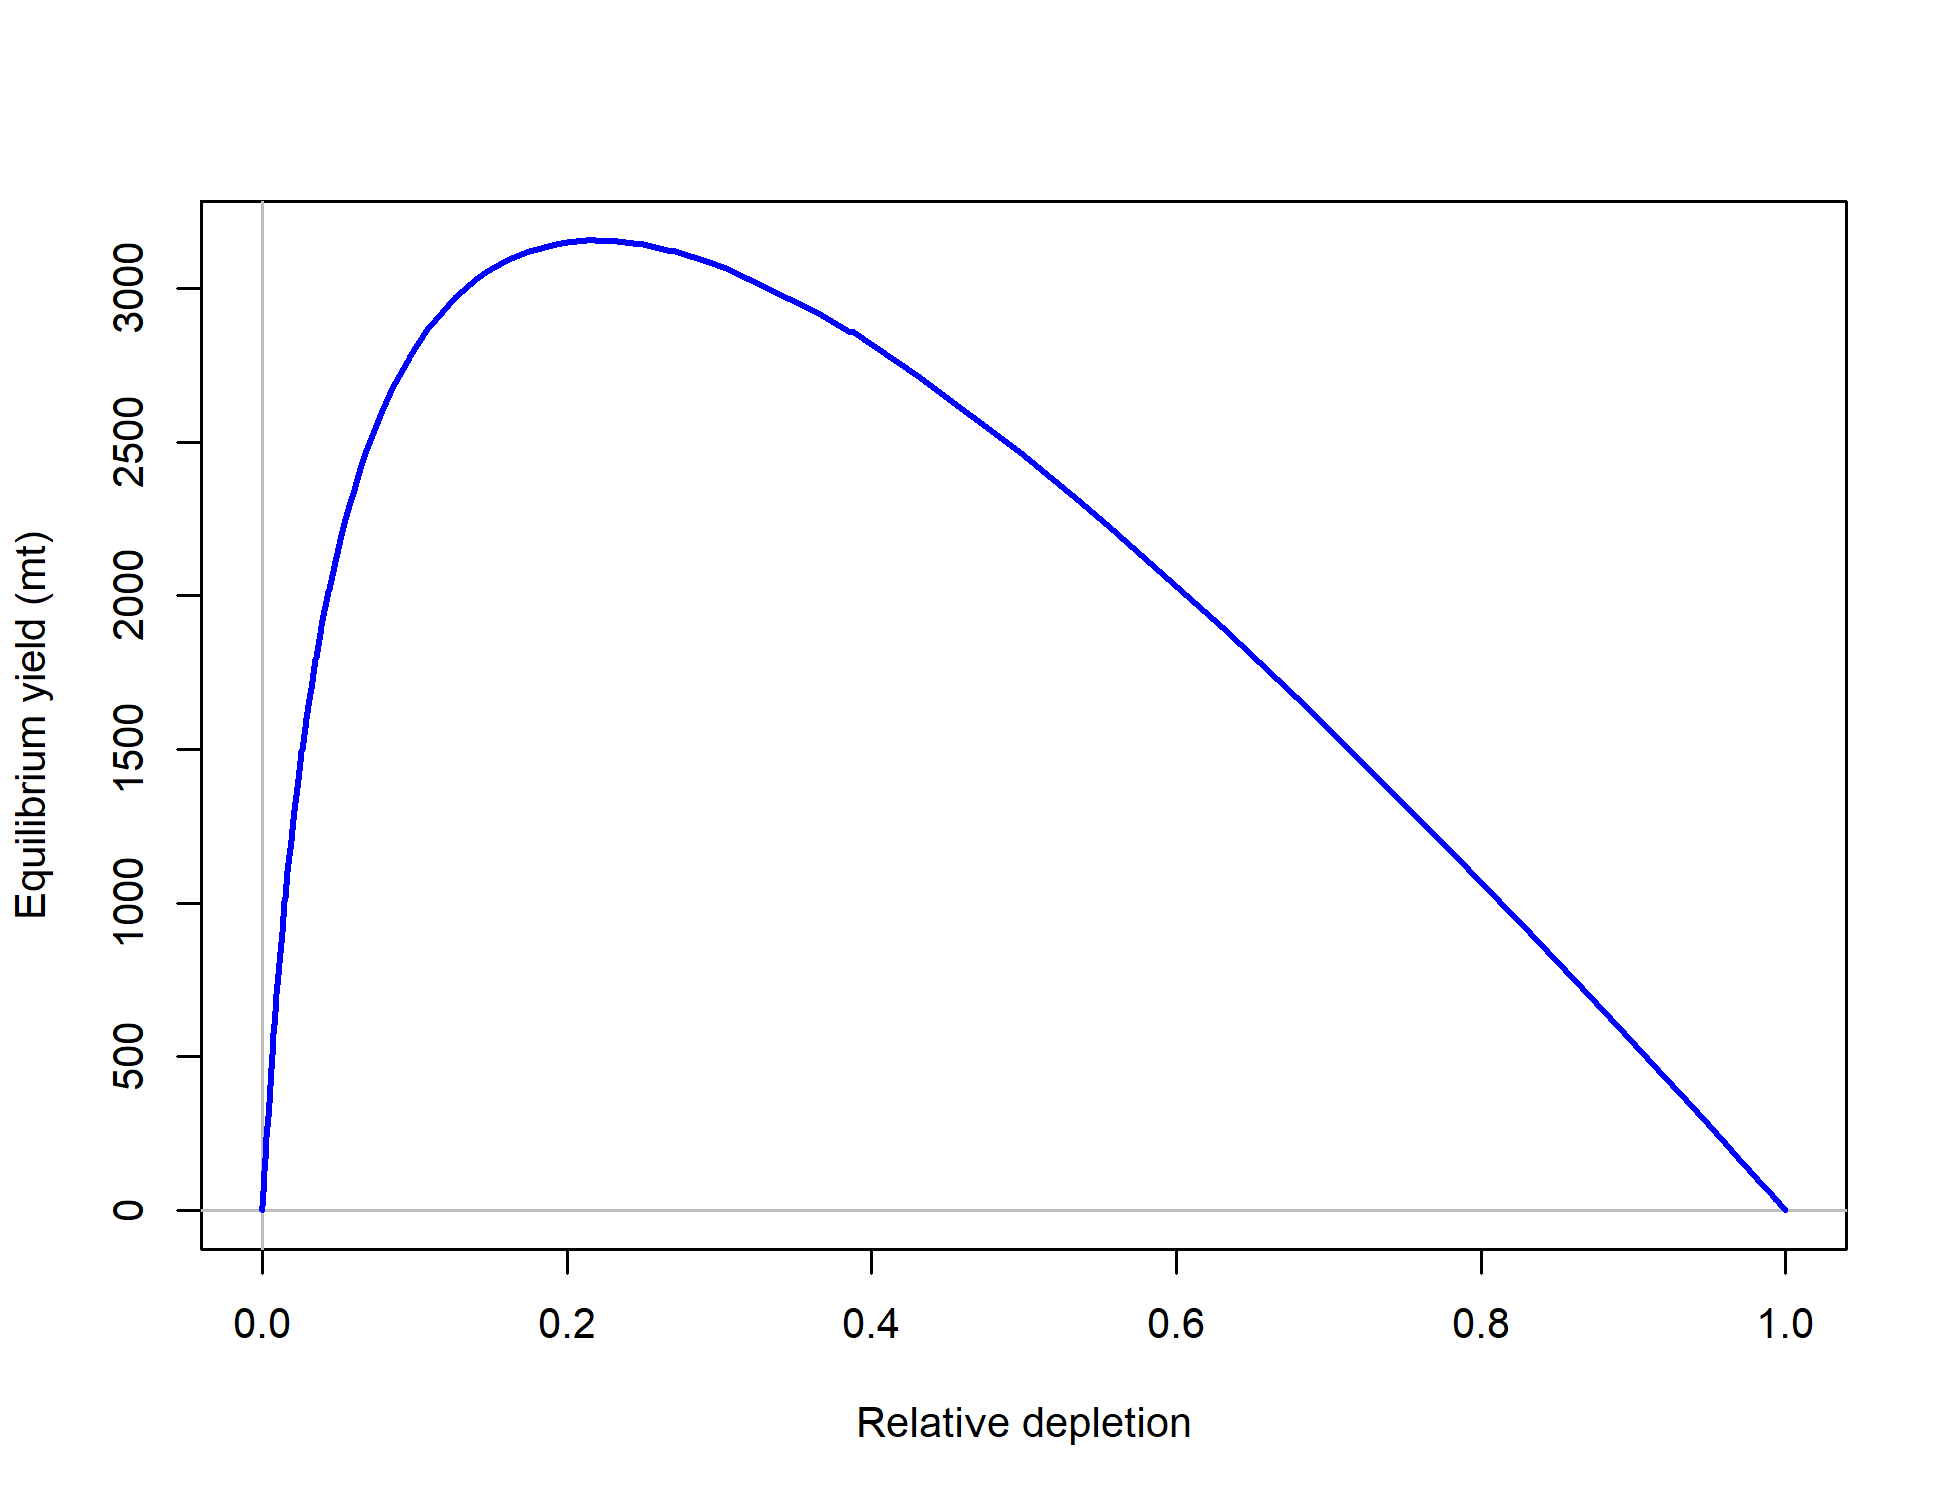
\includegraphics{r4ss/plots_mod1/yield1_yield_curve.png}
\caption{Equilibrium yield curve for the base case model. Values are
based on the 2018 fishery selectivity and with steepness fixed at 0.89.
\label{fig:Yield_all}}
\end{figure}

\FloatBarrier

\newpage

\renewcommand{\thefigure}{\arabic{figure}}
\renewcommand{\thetable}{\arabic{table}}

\setcounter{figure}{0} \setcounter{table}{0}

\pagenumbering{arabic}

\section{Introduction}\label{introduction}

\subsection{Distribution and Stock
Structure}\label{distribution-and-stock-structure}

\subsection{Historical and Current
Fishery}\label{historical-and-current-fishery}

\subsection{Summary of Management History and
Performance}\label{summary-of-management-history-and-performance}

\subsection{Fisheries off Canada and
Alaska}\label{fisheries-off-canada-and-alaska}

\section{Data}\label{data}

Data used in the Petrale sole assessment are summarized in Figure
\ref{fig:data_plot}. A description of each data source is provided
below.

\subsection{Fishery-Independent Data}\label{fishery-independent-data}

\subsubsection{Northwest Fisheries Science Center (NWFSC) Shelf-Slope
Survey}\label{northwest-fisheries-science-center-nwfsc-shelf-slope-survey}

\subsubsection{Northwest Fisheries Science Center (NWFSC) Slope
Survey}\label{northwest-fisheries-science-center-nwfsc-slope-survey}

\subsubsection{Triennial Shelf Survey}\label{triennial-shelf-survey}

The Triennial shelf survey was first conducted by the AFSC in 1977 and
spanned the time-frame from 1977-2004. The survey's design and sampling
methods are most recently described in Weinberg et al.
(\protect\hyperlink{ref-weinberg_estimation_2002}{2002}). Its basic
design was a series of equally-spaced transects from which searches for
tows in a specific depth range were initiated. The survey design has
changed slightly over the period of time. In general, all of the surveys
were conducted in the mid-summer through early fall: the 1977 survey was
conducted from early July through late September; the surveys from 1980
through 1989 ran from mid-July to late September; the 1992 survey
spanned from mid-July through early October; the 1995 survey was
conducted from early June to late August; the 1998 survey ran from early
June through early August; and the 2001 and 2004 surveys were conducted
in May-July.

Haul depths ranged from 91-457 m during the 1977 survey with no hauls
shallower than 91 m. The surveys in 1980, 1983, and 1986 covered the
West Coast south to \(36.8^\circ\) N latitude and a depth range of
55-366 m. The surveys in 1989 and 1992 covered the same depth range but
extended the southern range to \(34.5^\circ\) N (near Point Conception).
From 1995 through 2004, the surveys covered the depth range 55-500 m and
surveyed south to \(34.5^\circ\) N. In the final year of the Triennial
series, 2004, the NWFSC's Fishery Resource and Monitoring division
(FRAM) conducted the survey and followed very similar protocols as the
AFSC.

Although the Triennial shelf survey was used in the 2011 assessment, it
was not used in the final base model for the current assessment for a
number of reasons. First, there were concerns regarding the varying
sampling and targeting of specific species by year across the
time-series. Secondly, the Triennial shelf survey targeted the shelf of
the West Coast and would not be expected to sample well slope species
such as Petrale sole. There were limited observations of Petrale sole
relative to other surveys (e.g.~NWFSC shelf-slope survey) and the length
and age distributions varied in such a manner that would indicate either
poor sampling of Petrale sole or inconsistent sampling of the
population.

\subsection{Fishery-Dependent Data}\label{fishery-dependent-data}

\subsubsection{Commercial Fishery
Landings}\label{commercial-fishery-landings}

\textbf{Washington}

\textbf{Oregon}

\textbf{California}

\subsubsection{Discards}\label{discards}

Data on discards of Petrale sole are available from two different data
sources. The earliest source is referred to as the Pikitch data and
comes from a study organized by Ellen Pikitch that collected trawl
discards from 1985-1987 (Pikitch et al.
\protect\hyperlink{ref-pikitch_evaluation_1988}{1988}). The northern and
southern boundaries of the study were \(48^\circ 42^\prime\) N latitude
and \(42^\circ 60^\prime\) N latitude respectively, which is primarily
within the Columbia INPFC area (Pikitch et al.
\protect\hyperlink{ref-pikitch_evaluation_1988}{1988}, Rogers and
Pikitch \protect\hyperlink{ref-rogers_numerical_1992}{1992}).
Participation in the study was voluntary and included vessels using
bottom, midwater, and shrimp trawl gears. Observers of normal fishing
operations on commercial vessels collected the data, estimated the total
weight of the catch by tow, and recorded the weight of species retained
and discarded in the sample. Results of the Pikitch data were obtained
from John Wallace (personal communication, NWFSC, NOAA) in the form of
ratios of discard weight to retained weight of Petrale sole and
sex-specific length frequencies. Discard estimates are shown in Table
\ref{tab:Discard}.

The second source is from the West Coast Groundfish Observer Program
(WCGOP). This program is part of the NWFSC and has been recording
discard observations since 2003. Table \ref{tab:Discard} shows the
discard ratios (discarded/(discarded + retained)) of Petrale sole from
WCGOP. Since 2011, when the trawl rationalization program was
implemented, observer coverage rates increased to nearly 100\% for all
the limited entry trawl vessels in the program and discard rates
declined compared to pre-2011 rates. Discard rates were obtained for
both the catch-share and the non-catch share sector for Petrale sole. A
single discard rate was calculated by weighting discard rates based on
the commercial landings by each sector. Coefficient of variations were
calculated for the non-catch shares sector and pre-catch share years by
bootstrapping vessels within ports because the observer program randomly
chooses vessels within ports to be observed. Post-ITQ, all catch-share
vessels have 100\% observer coverage and discarding is assumed to be
known.

\subsubsection{Fishery Length and Age
Data}\label{fishery-length-and-age-data}

\paragraph{Commercial Fishery}\label{commercial-fishery}

\begin{centering}

Input effN = $N_{\text{trips}} + 0.138 * N_{\text{fish}}$ if $N_{\text{fish}}/N_{\text{trips}}$ is $<$ 44

Input effN = $7.06 * N_{\text{trips}}$ if $N_{\text{fish}}/N_{\text{trips}}$ is $\geq$ 44

\end{centering}

\subsubsection{Historical Commercial Catch-Per-Unit
Effort}\label{historical-commercial-catch-per-unit-effort}

\subsection{Biological Data}\label{biological-data}

\subsubsection{Natural Mortality}\label{natural-mortality}

\subsubsection{Sex Ratio, Maturation, and
Fecundity}\label{sex-ratio-maturation-and-fecundity}

\subsubsection{Length-Weight
Relationship}\label{length-weight-relationship}

\subsubsection{Growth (Length-at-Age)}\label{growth-length-at-age}

\subsubsection{Ageing Precision and
Bias}\label{ageing-precision-and-bias}

\subsection{History of Modeling Approaches Used for This
Stock}\label{history-of-modeling-approaches-used-for-this-stock}

\subsubsection{Previous Assessments}\label{previous-assessments}

\section{Assessment}\label{assessment}

\subsection{General Model Specifications and
Assumptions}\label{general-model-specifications-and-assumptions}

Stock Synthesis version 3.30.03.XX was used to estimate the parameters
in the model. R4SS, version 1.XX.X, along with R version 3.3.2 were used
to investigate and plot model fits. A summary of the data sources used
in the model (details discussed above) is shown in Figure
\ref{fig:data_plot}.

\subsubsection{Changes Between the 2015 Update Assessment Model and
Current
Model}\label{changes-between-the-2015-update-assessment-model-and-current-model}

\subsubsection{Summary of Fleets and
Areas}\label{summary-of-fleets-and-areas}

\subsubsection{Other Specifications}\label{other-specifications}

\subsubsection{Modeling Software}\label{modeling-software}

The STAT team used Stock Synthesis version 3.30.03.XX developed by
Dr.~Richard Methot at the NWFSC (Methot and Wetzel
\protect\hyperlink{ref-methot_stock_2013}{2013}). This most recent
version was used because it included improvements and corrections to
older versions.

\subsubsection{Priors}\label{priors}

\subsubsection{Data Weighting}\label{data-weighting}

\subsubsection{Estimated and Fixed
Parameters}\label{estimated-and-fixed-parameters}

\subsubsection{Key Assumptions and Structural
Choices}\label{key-assumptions-and-structural-choices}

\subsubsection{Bridging Analysis}\label{bridging-analysis}

\subsubsection{Convergence}\label{convergence}

\subsection{Base Model Results}\label{base-model-results}

\subsubsection{Parameter Estimates}\label{parameter-estimates}

\subsubsection{Fits to the Data}\label{fits-to-the-data}

\subsubsection{Population Trajectory}\label{population-trajectory}

\subsubsection{Uncertainty and Sensitivity
Analyses}\label{uncertainty-and-sensitivity-analyses}

\subsubsection{Retrospective Analysis}\label{retrospective-analysis}

\subsubsection{Historical Analysis}\label{historical-analysis}

\subsubsection{Likelihood Profiles}\label{likelihood-profiles}

\subsubsection{Reference Points}\label{reference-points-1}

\section{Harvest Projections and Decision
Tables}\label{harvest-projections-and-decision-tables}

\section{Regional Management
Considerations}\label{regional-management-considerations}

\section{Research Needs}\label{research-needs}

There are many areas of research that could be improved to benefit the
understanding and assessment of Petrale sole. Below, are issues that are
considered of importance.

\begin{enumerate}

\item \textbf{Natural mortality}: 



\end{enumerate}

\section{Acknowledgments}\label{acknowledgments}

Many people were instrumental in the successful completion of this
assessment and their contribution is greatly appreciated.

\newpage

\FloatBarrier

\section{Tables}\label{tables}

\begin{table}[ht]
\centering
\caption{Landings for each fleet for the modeled years.} 
\label{tab:Comm_Catch}
\begin{tabular}{>{\centering}p{.5in}>{\centering}p{.75in}>{\centering}p{.75in}>{\centering}p{.75in}>{\centering}p{.75in}}
  \hline
Year & Winter North & Summer North & Winter South & Summer South \\ 
  \hline
1875 & 0 & 0 & 0 & 0 \\ 
  1876 & 0 & 0 & 0 & 1 \\ 
  1877 & 0 & 0 & 0 & 1 \\ 
  1878 & 0 & 0 & 0 & 1 \\ 
  1879 & 0 & 0 & 0 & 1 \\ 
  1880 & 0 & 0 & 0 & 12 \\ 
  1881 & 0 & 0 & 0 & 22 \\ 
  1882 & 0 & 0 & 0 & 33 \\ 
  1883 & 0 & 0 & 0 & 43 \\ 
  1884 & 0 & 0 & 0 & 54 \\ 
  1885 & 0 & 0 & 0 & 64 \\ 
  1886 & 0 & 0 & 0 & 75 \\ 
  1887 & 0 & 0 & 0 & 85 \\ 
  1888 & 0 & 0 & 0 & 96 \\ 
  1889 & 0 & 0 & 0 & 106 \\ 
  1890 & 0 & 0 & 0 & 117 \\ 
  1891 & 0 & 0 & 0 & 128 \\ 
  1892 & 0 & 0 & 0 & 138 \\ 
  1893 & 0 & 0 & 0 & 149 \\ 
  1894 & 0 & 0 & 0 & 159 \\ 
  1895 & 0 & 0 & 0 & 170 \\ 
  1896 & 0 & 0 & 0 & 180 \\ 
  1897 & 0 & 0 & 0 & 191 \\ 
  1898 & 0 & 0 & 0 & 201 \\ 
  1899 & 0 & 0 & 0 & 212 \\ 
  1900 & 0 & 0 & 0 & 223 \\ 
  1901 & 0 & 0 & 0 & 233 \\ 
  1902 & 0 & 0 & 0 & 244 \\ 
  1903 & 0 & 0 & 0 & 254 \\ 
  1904 & 0 & 0 & 0 & 265 \\ 
  1905 & 0 & 0 & 0 & 275 \\ 
  1906 & 0 & 0 & 0 & 286 \\ 
  1907 & 0 & 0 & 0 & 296 \\ 
  1908 & 0 & 0 & 0 & 307 \\ 
  1909 & 0 & 0 & 0 & 318 \\ 
  1910 & 0 & 0 & 0 & 328 \\ 
  1911 & 0 & 0 & 0 & 339 \\ 
  1912 & 0 & 0 & 0 & 349 \\ 
  1913 & 0 & 0 & 0 & 360 \\ 
  1914 & 0 & 0 & 0 & 370 \\ 
   \hline
\end{tabular}
\end{table}

\begin{table}[ht]
\centering
\begin{tabular}{>{\centering}p{.5in}>{\centering}p{.75in}>{\centering}p{.75in}>{\centering}p{.75in}>{\centering}p{.75in}}
  \hline
Year & Winter North & Summer North & Winter South & Summer South \\ 
  \hline
1915 & 0 & 0 & 0 & 381 \\ 
  1916 & 0 & 0 & 0 & 386 \\ 
  1917 & 0 & 0 & 0 & 526 \\ 
  1918 & 0 & 0 & 0 & 424 \\ 
  1919 & 0 & 0 & 0 & 333 \\ 
  1920 & 0 & 0 & 0 & 230 \\ 
  1921 & 0 & 0 & 0 & 294 \\ 
  1922 & 0 & 0 & 0 & 425 \\ 
  1923 & 0 & 0 & 0 & 427 \\ 
  1924 & 0 & 0 & 0 & 533 \\ 
  1925 & 0 & 0 & 0 & 528 \\ 
  1926 & 0 & 0 & 0 & 522 \\ 
  1927 & 0 & 0 & 0 & 632 \\ 
  1928 & 0 & 0 & 0 & 620 \\ 
  1929 & 0 & 2 & 0 & 706 \\ 
  1930 & 0 & 1 & 0 & 659 \\ 
  1931 & 0 & 81 & 63 & 531 \\ 
  1932 & 2 & 251 & 36 & 520 \\ 
  1933 & 6 & 408 & 39 & 392 \\ 
  1934 & 10 & 568 & 139 & 896 \\ 
  1935 & 14 & 650 & 155 & 777 \\ 
  1936 & 16 & 770 & 95 & 432 \\ 
  1937 & 20 & 1051 & 75 & 741 \\ 
  1938 & 27 & 1187 & 48 & 890 \\ 
  1939 & 35 & 1545 & 31 & 1029 \\ 
  1940 & 39 & 1737 & 162 & 597 \\ 
  1941 & 41 & 1803 & 111 & 331 \\ 
  1942 & 46 & 2919 & 24 & 216 \\ 
  1943 & 51 & 2867 & 72 & 345 \\ 
  1944 & 55 & 2047 & 86 & 447 \\ 
  1945 & 60 & 1866 & 102 & 439 \\ 
  1946 & 64 & 2492 & 72 & 1116 \\ 
  1947 & 69 & 1778 & 154 & 1093 \\ 
  1948 & 74 & 2315 & 273 & 1778 \\ 
  1949 & 76 & 1809 & 617 & 1812 \\ 
  1950 & 156 & 2322 & 424 & 1638 \\ 
  1951 & 118 & 1666 & 208 & 993 \\ 
  1952 & 131 & 1390 & 326 & 882 \\ 
  1953 & 46 & 737 & 533 & 981 \\ 
  1954 & 27 & 903 & 801 & 1073 \\ 
   \hline
\end{tabular}
\end{table}

\begin{table}[ht]
\centering
\begin{tabular}{>{\centering}p{.5in}>{\centering}p{.75in}>{\centering}p{.75in}>{\centering}p{.75in}>{\centering}p{.75in}}
  \hline
Year & Winter North & Summer North & Winter South & Summer South \\ 
  \hline
1955 & 57 & 863 & 526 & 1052 \\ 
  1956 & 137 & 759 & 508 & 801 \\ 
  1957 & 171 & 1103 & 527 & 1027 \\ 
  1958 & 99 & 1152 & 568 & 957 \\ 
  1959 & 332 & 947 & 379 & 723 \\ 
  1960 & 241 & 1374 & 520 & 644 \\ 
  1961 & 217 & 1547 & 542 & 1029 \\ 
  1962 & 295 & 1512 & 515 & 859 \\ 
  1963 & 663 & 1038 & 534 & 978 \\ 
  1964 & 282 & 1090 & 378 & 927 \\ 
  1965 & 370 & 950 & 374 & 853 \\ 
  1966 & 366 & 972 & 325 & 925 \\ 
  1967 & 409 & 793 & 532 & 874 \\ 
  1968 & 284 & 811 & 361 & 871 \\ 
  1969 & 190 & 887 & 421 & 848 \\ 
  1970 & 412 & 1081 & 472 & 1071 \\ 
  1971 & 743 & 883 & 540 & 1016 \\ 
  1972 & 730 & 1017 & 703 & 1000 \\ 
  1973 & 497 & 1272 & 417 & 742 \\ 
  1974 & 517 & 1611 & 665 & 893 \\ 
  1975 & 539 & 1559 & 561 & 901 \\ 
  1976 & 506 & 951 & 713 & 737 \\ 
  1977 & 682 & 743 & 484 & 495 \\ 
  1978 & 746 & 1098 & 419 & 801 \\ 
  1979 & 734 & 1086 & 353 & 945 \\ 
  1980 & 382 & 976 & 518 & 680 \\ 
  1981 & 761 & 468 & 360 & 895 \\ 
  1982 & 1041 & 771 & 262 & 502 \\ 
  1983 & 696 & 935 & 273 & 361 \\ 
  1984 & 416 & 739 & 260 & 329 \\ 
  1985 & 392 & 553 & 273 & 471 \\ 
  1986 & 474 & 714 & 403 & 355 \\ 
  1987 & 854 & 573 & 311 & 556 \\ 
  1988 & 743 & 610 & 349 & 411 \\ 
  1989 & 696 & 583 & 393 & 415 \\ 
  1990 & 641 & 460 & 319 & 373 \\ 
  1991 & 793 & 397 & 448 & 310 \\ 
  1992 & 640 & 366 & 272 & 307 \\ 
  1993 & 685 & 392 & 237 & 234 \\ 
  1994 & 518 & 355 & 246 & 299 \\ 
   \hline
\end{tabular}
\end{table}

\begin{table}[ht]
\centering
\begin{tabular}{>{\centering}p{.5in}>{\centering}p{.75in}>{\centering}p{.75in}>{\centering}p{.75in}>{\centering}p{.75in}}
  \hline
Year & Winter North & Summer North & Winter South & Summer South \\ 
  \hline
1915 & 0 & 0 & 0 & 381 \\ 
  1916 & 0 & 0 & 0 & 386 \\ 
  1917 & 0 & 0 & 0 & 526 \\ 
  1918 & 0 & 0 & 0 & 424 \\ 
  1919 & 0 & 0 & 0 & 333 \\ 
  1920 & 0 & 0 & 0 & 230 \\ 
  1921 & 0 & 0 & 0 & 294 \\ 
  1922 & 0 & 0 & 0 & 425 \\ 
  1923 & 0 & 0 & 0 & 427 \\ 
  1924 & 0 & 0 & 0 & 533 \\ 
  1925 & 0 & 0 & 0 & 528 \\ 
  1926 & 0 & 0 & 0 & 522 \\ 
  1927 & 0 & 0 & 0 & 632 \\ 
  1928 & 0 & 0 & 0 & 620 \\ 
  1929 & 0 & 2 & 0 & 706 \\ 
  1930 & 0 & 1 & 0 & 659 \\ 
  1931 & 0 & 81 & 63 & 531 \\ 
  1932 & 2 & 251 & 36 & 520 \\ 
  1933 & 6 & 408 & 39 & 392 \\ 
  1934 & 10 & 568 & 139 & 896 \\ 
  1935 & 14 & 650 & 155 & 777 \\ 
  1936 & 16 & 770 & 95 & 432 \\ 
  1937 & 20 & 1051 & 75 & 741 \\ 
  1938 & 27 & 1187 & 48 & 890 \\ 
  1939 & 35 & 1545 & 31 & 1029 \\ 
  1940 & 39 & 1737 & 162 & 597 \\ 
  1941 & 41 & 1803 & 111 & 331 \\ 
  1942 & 46 & 2919 & 24 & 216 \\ 
  1943 & 51 & 2867 & 72 & 345 \\ 
  1944 & 55 & 2047 & 86 & 447 \\ 
  1945 & 60 & 1866 & 102 & 439 \\ 
  1946 & 64 & 2492 & 72 & 1116 \\ 
  1947 & 69 & 1778 & 154 & 1093 \\ 
  1948 & 74 & 2315 & 273 & 1778 \\ 
  1949 & 76 & 1809 & 617 & 1812 \\ 
  1950 & 156 & 2322 & 424 & 1638 \\ 
  1951 & 118 & 1666 & 208 & 993 \\ 
  1952 & 131 & 1390 & 326 & 882 \\ 
  1953 & 46 & 737 & 533 & 981 \\ 
  1954 & 27 & 903 & 801 & 1073 \\ 
   \hline
\end{tabular}
\end{table}

\begin{table}[ht]
\centering
\begin{tabular}{>{\centering}p{.5in}>{\centering}p{.75in}>{\centering}p{.75in}>{\centering}p{.75in}>{\centering}p{.75in}}
  \hline
Year & Winter North & Summer North & Winter South & Summer South \\ 
  \hline
1995 & 591 & 454 & 236 & 287 \\ 
  1996 & 591 & 440 & 406 & 394 \\ 
  1997 & 621 & 430 & 448 & 442 \\ 
  1998 & 522 & 577 & 221 & 300 \\ 
  1999 & 463 & 504 & 287 & 267 \\ 
  2000 & 610 & 586 & 374 & 241 \\ 
  2001 & 691 & 597 & 308 & 260 \\ 
  2002 & 667 & 714 & 335 & 195 \\ 
  2003 & 544 & 713 & 256 & 180 \\ 
  2004 & 1010 & 750 & 177 & 267 \\ 
  2005 & 964 & 1069 & 337 & 533 \\ 
  2006 & 537 & 1012 & 125 & 454 \\ 
  2007 & 930 & 536 & 404 & 475 \\ 
  2008 & 842 & 354 & 519 & 414 \\ 
  2009 & 847 & 642 & 470 & 250 \\ 
  2010 & 258 & 292 & 78 & 121 \\ 
  2011 & 222 & 423 & 40 & 78 \\ 
  2012 & 406 & 478 & 124 & 108 \\ 
  2013 & 509 & 1007 & 130 & 278 \\ 
  2014 & 853 & 860 & 273 & 354 \\ 
  2015 & 0 & 0 & 0 & 10 \\ 
  2016 & 0 & 0 & 0 & 10 \\ 
  2017 & 0 & 0 & 0 & 10 \\ 
  2018 & 0 & 0 & 0 & 10 \\ 
   \hline
\end{tabular}
\end{table}

\begin{table}[ht]
\centering
\caption{Recent trend in estimated total catch relative to management guidelines. The estimated total catch includes the total landings plus the model estimated discard mortality based upon discard rate data.} 
\label{tab:mnmgt_perform_tables}
\begin{tabular}{>{\raggedleft}p{0.5in}>{\centering}p{1.0in}>{\centering}p{1.0in}>{\centering}p{1.1in}>{\centering}p{1.1in}}
  \hline
Year & OFL (mt; ABC prior to 2011) & ACL (mt; OY prior to 2011) & Total landings (mt) & Estimated total catch (mt) \\ 
  \hline
\text{2009} & 2,811 & 2433 & 2208 & 2323 \\ 
  \text{2010} & 2,751 & 1200 & 749 & 914 \\ 
  \text{2011} & 1,021 & 976 & 762 & 781 \\ 
  \text{2012} & 1,275 & 1160 & 1116 & 1135 \\ 
  \text{2013} & 2,711 & 2592 & 1925 & 1954 \\ 
  \text{2014} & 2,774 & 2652 & 2341 & 2361 \\ 
  \text{2015} & 3,073 & 2816 & 10 & 10 \\ 
  \text{2016} & 3,208 & 2910 & 10 & 10 \\ 
  \text{2017} & 3,208 & 3,136 & 10 & 10 \\ 
  \text{2018} & 3,152 & 3,013 & 10 & 10 \\ 
   \hline
\end{tabular}
\end{table}

\begin{table}[ht]
\centering
\caption{Description of the data used to create the indices, the modeling platform used to generate the estimates, and the model configuration.} 
\label{tab:strata}
\begin{tabular}{>{\centering}p{1.10in}>{\centering}p{1.10in}>{\centering}p{1.10in}>{\centering}p{1.10in}}
  \hline
 & Early Triennial & Late Triennial & NWFS Shelf-Slope \\ 
  \hline
Depth & 55-100, 100-400 & 55- 100, 100-500 & 55-100, 100-183, 183-549 \\ 
  Latitude & INPFC & INPFC & INPFC \\ 
  Model & VAST & VAST & VAST \\ 
  Error Structure &  &  &  \\ 
  Knots &  &  &  \\ 
  Spatial & Y &  & Y \\ 
  Temporal & Y &  & Y \\ 
  Vessel-Year & N &  & Y \\ 
   \hline
\end{tabular}
\end{table}

\begin{table}[ht]
\centering
\caption{Description of the strata used to create the indices for the NWFSC Shelf-Slope survey.} 
\label{tab:strata_nwfsc}
\begin{tabular}{>{\raggedright}p{1.5in}>{\centering}p{0.50in}>{\centering}p{0.50in}>{\centering}p{0.50in}>{\centering}p{0.50in}}
  \hline
Strata & Depth Lower Bound & Depth Upper Bound & Latitude South & Latitude North \\ 
  \hline
Shallow Vancouver &  55 & 100 & 47.00 & 49.00 \\ 
  Shallow Columbia &  55 & 100 & 43.00 & 47.00 \\ 
  Shallow Eureka &  55 & 100 & 40.50 & 43.00 \\ 
  Shallow Monterey &  55 & 100 & 38.00 & 40.50 \\ 
  Shallow Conception &  55 & 100 & 34.50 & 38.00 \\ 
  Mid Vancouver & 100 & 183 & 47.00 & 49.00 \\ 
  Mid Columbia & 100 & 183 & 43.00 & 47.00 \\ 
  Mid Eureka & 100 & 183 & 40.50 & 43.00 \\ 
  Mid Monterey & 100 & 183 & 38.00 & 40.50 \\ 
  Mid Conception & 100 & 183 & 34.50 & 38.00 \\ 
  Deep Van/Col/Eur & 183 & 549 & 40.50 & 49.00 \\ 
  Deep Montery & 183 & 549 & 38.00 & 40.50 \\ 
  Deep Conception & 183 & 549 & 34.50 & 38.00 \\ 
   \hline
\end{tabular}
\end{table}

\begin{table}[ht]
\centering
\caption{Description of the strata used to create the indices for the Triennial Early (1980 - 1992) survey.} 
\label{tab:strata_tri_early}
\begin{tabular}{>{\raggedright}p{1.5in}>{\centering}p{0.50in}>{\centering}p{0.50in}>{\centering}p{0.50in}>{\centering}p{0.50in}}
  \hline
Strata & Depth Lower Bound & Depth Upper Bound & Latitude South & Latitude North \\ 
  \hline
Shallow Van/Col &  55 & 100 & 43.00 & 49.00 \\ 
  Shallow Eureka &  55 & 100 & 40.50 & 43.00 \\ 
  Shallow Mon/Con &  55 & 100 & 34.50 & 40.50 \\ 
  Deep Van/Col/Eur & 100 & 400 & 40.50 & 49.00 \\ 
  Deep Mon/Con & 100 & 400 & 34.50 & 40.50 \\ 
   \hline
\end{tabular}
\end{table}

\begin{table}[ht]
\centering
\caption{Description of the strata used to create the indices for the Triennial Late (1995-2004) survey.} 
\label{tab:strata_tri_late}
\begin{tabular}{>{\raggedright}p{1.5in}>{\centering}p{0.50in}>{\centering}p{0.50in}>{\centering}p{0.50in}>{\centering}p{0.50in}}
  \hline
Strata & Depth Lower Bound & Depth Upper Bound & Latitude South & Latitude North \\ 
  \hline
Shallow Van/Col &  55 & 100 & 43.00 & 49.00 \\ 
  Shallow Eureka &  55 & 100 & 40.50 & 43.00 \\ 
  Shallow Mon/Con &  55 & 100 & 34.50 & 40.50 \\ 
  Deep Van/Col & 100 & 500 & 43.00 & 49.00 \\ 
  Deep Eureka & 100 & 500 & 40.50 & 43.00 \\ 
  Deep Mon/Con & 100 & 500 & 34.50 & 40.50 \\ 
   \hline
\end{tabular}
\end{table}

\begin{table}[ht]
\centering
\caption{Summary of the fishery-independent biomass/abundance
                                         time-series used in the stock
                                         assessment.  The standard error includes the input annual standard error and model estimated added variance.} 
\label{tab:Index_Summary}
\begin{tabular}{>{\centering}p{.4in}>{\centering}p{.5in}>{\centering}p{.3in}>{\centering}p{.5in}>{\centering}p{.3in}>{\centering}p{.5in}>{\centering}p{.3in}>{\centering}p{.5in}>{\centering}p{.3in}>{\centering}p{.5in}>{\centering}p{.3in}}
  \hline
   & \multicolumn{2}{c}{Winter N.} &  \multicolumn{2}{c}{Winter S.} & \multicolumn{2}{c}{Triennial Early} & \multicolumn{2}{c}{Triennial Late} & \multicolumn{2}{c}{NWFSC Combo} \\
 Year & Obs & SE & Obs & SE & Obs & SE & Obs & SE & Obs & SE\\
 \hline
1980 & - & - & - & - & 1864 & 0.49 & - & - & - & - \\ 
  1983 & - & - & - & - & 2300 & 0.29 & - & - & - & - \\ 
  1986 & - & - & - & - & 2193 & 0.31 & - & - & - & - \\ 
  1987 & 1.09 & 0.28 & 1.08 & 0.56 & - & - & - & - & - & - \\ 
  1988 & 1.16 & 0.27 & 0.91 & 0.33 & - & - & - & - & - & - \\ 
  1989 & 0.92 & 0.27 & 0.53 & 0.43 & 3234 & 0.27 & - & - & - & - \\ 
  1990 & 0.76 & 0.28 & 0.96 & 0.46 & - & - & - & - & - & - \\ 
  1991 & 0.86 & 0.27 & 0.90 & 0.36 & - & - & - & - & - & - \\ 
  1992 & 0.56 & 0.28 & 0.59 & 0.68 & 2126 & 0.28 & - & - & - & - \\ 
  1993 & 0.56 & 0.27 & 0.86 & 0.35 & - & - & - & - & - & - \\ 
  1994 & 0.50 & 0.28 & 0.71 & 0.30 & - & - & - & - & - & - \\ 
  1995 & 0.66 & 0.28 & 0.90 & 0.30 & - & - & 2407 & 0.33 & - & - \\ 
  1996 & 0.77 & 0.29 & 1.25 & 0.30 & - & - & - & - & - & - \\ 
  1997 & 0.85 & 0.28 & 0.82 & 0.28 & - & - & - & - & - & - \\ 
  1998 & 1.01 & 0.29 & 0.93 & 0.31 & - & - & 3548 & 0.30 & - & - \\ 
  1999 & 0.71 & 0.29 & 0.83 & 0.29 & - & - & - & - & - & - \\ 
  2000 & 0.67 & 0.28 & 0.62 & 0.29 & - & - & - & - & - & - \\ 
  2001 & 0.83 & 0.27 & 0.66 & 0.29 & - & - & 3832 & 0.30 & - & - \\ 
  2002 & 0.93 & 0.28 & 0.80 & 0.29 & - & - & - & - & - & - \\ 
  2003 & 1.02 & 0.28 & 0.85 & 0.29 & - & - & - & - & 18698 & 0.13 \\ 
  2004 & 1.63 & 0.28 & 1.71 & 0.31 & - & - & 9713 & 0.32 & 22866 & 0.12 \\ 
  2005 & 1.85 & 0.28 & 1.93 & 0.29 & - & - & - & - & 22056 & 0.11 \\ 
  2006 & 2.01 & 0.28 & 1.58 & 0.29 & - & - & - & - & 19276 & 0.12 \\ 
  2007 & 2.04 & 0.28 & 2.07 & 0.28 & - & - & - & - & 19428 & 0.12 \\ 
  2008 & 1.96 & 0.27 & 1.62 & 0.28 & - & - & - & - & 15981 & 0.12 \\ 
  2009 & 2.12 & 0.27 & 1.76 & 0.28 & - & - & - & - & 15893 & 0.12 \\ 
  2010 & - & - & - & - & - & - & - & - & 22700 & 0.11 \\ 
  2011 & - & - & - & - & - & - & - & - & 30022 & 0.10 \\ 
  2012 & - & - & - & - & - & - & - & - & 36628 & 0.12 \\ 
  2013 & - & - & - & - & - & - & - & - & 51165 & 0.12 \\ 
  2014 & - & - & - & - & - & - & - & - & 58504 & 0.11 \\ 
   \hline
\end{tabular}
\end{table}

\FloatBarrier

\begin{table}[ht]
\centering
\caption{Summary of NWFSC shelf-slope survey length samples used in the stock assessment. The sample sizes were calculated according to                              Stewart and Hamel (2014), which determined that the approximate realized sample size for flatfish species was 3.09 fish per tow.} 
\label{tab:NWcombo_Lengths}
\begin{tabular}{>{\centering}p{.75in}>{\centering}p{.75in}>{\centering}p{.75in}>{\centering}p{1in}}
  \hline
Year & Tows & Fish & Sample Size \\ 
  \hline
2003 & 46 & 1426 & 111 \\ 
  2004 & 34 & 565 & 82 \\ 
  2005 & 38 & 526 & 92 \\ 
  2006 & 33 & 659 & 80 \\ 
  2007 & 50 & 628 & 121 \\ 
  2008 & 39 & 539 & 94 \\ 
  2009 & 46 & 471 & 111 \\ 
  2010 & 53 & 907 & 128 \\ 
  2011 & 53 & 921 & 128 \\ 
  2012 & 50 & 1175 & 121 \\ 
  2013 & 45 & 732 & 109 \\ 
  2014 & 52 & 991 & 126 \\ 
  2015 & 69 & 1165 & 167 \\ 
  2016 & 50 & 1150 & 121 \\ 
   \hline
\end{tabular}
\end{table}

\begin{table}[ht]
\centering
\caption{Summary of NWFSC shelf-slope survey age samples used in the stock assessment. The sample sizes were calculated according to                              Stewart and Hamel (2014), which determined that the approximate realized sample size for flatfish species was 3.09 fish per tow.} 
\label{tab:NWcombo_Ages}
\begin{tabular}{>{\centering}p{.75in}>{\centering}p{.75in}>{\centering}p{.75in}>{\centering}p{1in}}
  \hline
Year & Tows & Fish & Sample Size \\ 
  \hline
2003 & 45 & 432 & 109 \\ 
  2004 & 34 & 219 & 82 \\ 
  2005 & 38 & 257 & 92 \\ 
  2006 & 33 & 254 & 80 \\ 
  2007 & 50 & 439 & 121 \\ 
  2008 & 39 & 328 & 94 \\ 
  2009 & 45 & 331 & 109 \\ 
  2010 & 53 & 579 & 128 \\ 
  2011 & 53 & 674 & 128 \\ 
  2012 & 49 & 699 & 119 \\ 
  2013 & 44 & 553 & 106 \\ 
  2014 & 52 & 626 & 126 \\ 
  2015 & 68 & 840 & 165 \\ 
  2016 & 44 & 703 & 106 \\ 
   \hline
\end{tabular}
\end{table}

\begin{table}[ht]
\centering
\caption{Summary of Triennial survey length samples used in the stock assessment. The sample sizes were calculated according to                              Stewart and Hamel (2014), which determined that the approximate realized sample size for flatfish species was 3.09 fish per tow.} 
\label{tab:Triennial_Lengths}
\begin{tabular}{>{\centering}p{.75in}>{\centering}p{.75in}>{\centering}p{.75in}>{\centering}p{1in}}
  \hline
Year & Tows & Fish & Sample Size \\ 
  \hline
1980 & 18 & 1315 & 43 \\ 
  1983 & 40 & 2820 & 97 \\ 
  1986 & 17 & 877 & 41 \\ 
  1989 & 42 & 1851 & 102 \\ 
  1992 & 33 & 1182 & 80 \\ 
  1995 & 71 & 1136 & 172 \\ 
  1998 & 81 & 1482 & 196 \\ 
  2001 & 74 & 669 & 179 \\ 
  2004 & 63 & 1240 & 153 \\ 
   \hline
\end{tabular}
\end{table}

\begin{table}[ht]
\centering
\caption{Summary of discard rates used in the model by each data source (continued on next page).} 
\label{tab:Discard}
\begin{tabular}{>{\centering}p{.75in}>{\centering}p{1.1in}>{\centering}p{.75in}>{\centering}p{1.1in}}
  \hline
Year & Source & Discard Rate & Standard Error \\ 
  \hline
2007 & WinterN & 0.004 & 0.002 \\ 
  2004 & WinterN & 0.001 & 0.001 \\ 
  2008 & WinterN & 0.028 & 0.014 \\ 
  2005 & WinterN & 0.001 & 0.000 \\ 
  2002 & WinterN & 0.007 & 0.003 \\ 
  2009 & WinterN & 0.027 & 0.016 \\ 
  2006 & WinterN & 0.012 & 0.021 \\ 
  2003 & WinterN & 0.007 & 0.019 \\ 
  2010 & WinterN & 0.209 & 0.054 \\ 
  2011 & WinterN & 0.001 & 0.021 \\ 
  2012 & WinterN & 0.001 & 0.021 \\ 
  2013 & WinterN & 0.001 & 0.021 \\ 
  2014 & WinterN & 0.002 & 0.021 \\ 
  1985 & WinterN & 0.022 & 0.110 \\ 
  1986 & WinterN & 0.021 & 0.116 \\ 
  1987 & WinterN & 0.027 & 0.119 \\ 
  2004 & SummerN & 0.091 & 0.032 \\ 
  2005 & SummerN & 0.040 & 0.009 \\ 
  2002 & SummerN & 0.212 & 0.027 \\ 
  2006 & SummerN & 0.078 & 0.017 \\ 
  2003 & SummerN & 0.145 & 0.090 \\ 
  2007 & SummerN & 0.107 & 0.020 \\ 
  2008 & SummerN & 0.054 & 0.011 \\ 
  2009 & SummerN & 0.202 & 0.062 \\ 
  2010 & SummerN & 0.089 & 0.026 \\ 
  2011 & SummerN & 0.032 & 0.021 \\ 
  2012 & SummerN & 0.015 & 0.021 \\ 
  2013 & SummerN & 0.023 & 0.021 \\ 
  1985 & SummerN & 0.035 & 0.042 \\ 
  1986 & SummerN & 0.034 & 0.043 \\ 
  1987 & SummerN & 0.032 & 0.045 \\ 
   \hline
\end{tabular}
\end{table}

\begin{table}[ht]
\centering
\begin{tabular}{>{\centering}p{.75in}>{\centering}p{1.1in}>{\centering}p{.75in}>{\centering}p{1.1in}}
  \hline
Year & Source & Discard Rate & Standard Error \\ 
  \hline
2002 & WinterS & 0.035 & 0.025 \\ 
  2003 & WinterS & 0.006 & 0.003 \\ 
  2004 & WinterS & 0.025 & 0.052 \\ 
  2005 & WinterS & 0.006 & 0.006 \\ 
  2009 & WinterS & 0.021 & 0.015 \\ 
  2006 & WinterS & 0.075 & 0.043 \\ 
  2010 & WinterS & 0.278 & 0.060 \\ 
  2007 & WinterS & 0.018 & 0.014 \\ 
  2008 & WinterS & 0.010 & 0.006 \\ 
  2011 & WinterS & 0.001 & 0.021 \\ 
  2012 & WinterS & 0.003 & 0.021 \\ 
  2013 & WinterS & 0.000 & 0.021 \\ 
  2014 & WinterS & 0.000 & 0.021 \\ 
  2002 & SummerS & 0.058 & 0.016 \\ 
  2009 & SummerS & 0.023 & 0.008 \\ 
  2006 & SummerS & 0.038 & 0.016 \\ 
  2003 & SummerS & 0.036 & 0.013 \\ 
  2010 & SummerS & 0.056 & 0.012 \\ 
  2007 & SummerS & 0.065 & 0.021 \\ 
  2004 & SummerS & 0.033 & 0.015 \\ 
  2008 & SummerS & 0.026 & 0.015 \\ 
  2005 & SummerS & 0.012 & 0.003 \\ 
  2011 & SummerS & 0.041 & 0.021 \\ 
  2012 & SummerS & 0.013 & 0.021 \\ 
  2013 & SummerS & 0.004 & 0.021 \\ 
   \hline
\end{tabular}
\end{table}

\begin{table}[ht]
\centering
\caption{Summary of Winter North fishery length samples used in the stock assessment (continued on next page). Sample sizes were calculated according to method described above in Section \ref{fishery-length-and-age-data}.} 
\label{tab:WN_Lengths}
\begingroup\fontsize{11pt}{11pt}\selectfont
\begin{tabular}{>{\centering}p{.75in}>{\centering}p{.75in}>{\centering}p{.75in}>{\centering}p{1in}}
  \hline
Year & Trips & Fish & Sample Size \\ 
  \hline
1966 & 1 & 238 & 7 \\ 
  1967 & 5 & 1020 & 35 \\ 
  1968 & 3 & 912 & 21 \\ 
  1969 & 4 & 1213 & 28 \\ 
  1970 & 13 & 1830 & 92 \\ 
  1971 & 22 & 4698 & 155 \\ 
  1972 & 23 & 4561 & 162 \\ 
  1973 & 17 & 4134 & 120 \\ 
  1974 & 20 & 4806 & 141 \\ 
  1975 & 19 & 3637 & 134 \\ 
  1976 & 21 & 3677 & 148 \\ 
  1977 & 32 & 4846 & 226 \\ 
  1978 & 52 & 7715 & 367 \\ 
  1979 & 34 & 3414 & 240 \\ 
  1980 & 55 & 5425 & 388 \\ 
  1981 & 40 & 3921 & 282 \\ 
  1982 & 48 & 4824 & 339 \\ 
  1983 & 39 & 3944 & 275 \\ 
  1984 & 31 & 3102 & 219 \\ 
  1985 & 45 & 4508 & 318 \\ 
  1986 & 40 & 4002 & 282 \\ 
  1987 & 43 & 3053 & 304 \\ 
  1988 & 9 & 601 & 64 \\ 
  1989 & 16 & 798 & 113 \\ 
  1990 & 12 & 599 & 85 \\ 
  1991 & 8 & 216 & 38 \\ 
  1994 & 43 & 2608 & 304 \\ 
  1995 & 49 & 3161 & 346 \\ 
  1996 & 64 & 3085 & 452 \\ 
  1997 & 76 & 3570 & 537 \\ 
  1998 & 56 & 3450 & 395 \\ 
  1999 & 58 & 2812 & 409 \\ 
  2000 & 49 & 2004 & 326 \\ 
  2001 & 59 & 1696 & 293 \\ 
  2002 & 50 & 1666 & 280 \\ 
  2003 & 67 & 1661 & 296 \\ 
  2004 & 53 & 1202 & 219 \\ 
  2005 & 51 & 1277 & 227 \\ 
  2006 & 59 & 1486 & 264 \\ 
  2007 & 81 & 2248 & 391 \\ 
  2008 & 101 & 3058 & 523 \\ 
  2009 & 107 & 3207 & 550 \\ 
  2010 & 134 & 2872 & 530 \\ 
  2011 & 100 & 1943 & 368 \\ 
  2012 & 97 & 1873 & 355 \\ 
  2013 & 117 & 2167 & 416 \\ 
  2014 & 140 & 2850 & 533 \\ 
  2015 & 110 & 2504 & 456 \\ 
  2016 & 131 & 2158 & 429 \\ 
   \hline
\end{tabular}
\endgroup
\end{table}

\begin{table}[ht]
\centering
\caption{Summary of Summer North fishery length samples used in the stock assessment (continued on next page). Sample sizes were calculated according to method described above in Section \ref{fishery-length-and-age-data}.} 
\label{tab:SN_Lengths}
\begingroup\fontsize{11pt}{11pt}\selectfont
\begin{tabular}{>{\centering}p{.75in}>{\centering}p{.75in}>{\centering}p{.75in}>{\centering}p{1in}}
  \hline
Year & Trips & Fish & Sample Size \\ 
  \hline
1966 & 1 & 238 & 7 \\ 
  1967 & 5 & 1020 & 35 \\ 
  1968 & 3 & 912 & 21 \\ 
  1969 & 4 & 1213 & 28 \\ 
  1970 & 13 & 1830 & 92 \\ 
  1971 & 22 & 4698 & 155 \\ 
  1972 & 23 & 4561 & 162 \\ 
  1973 & 17 & 4134 & 120 \\ 
  1974 & 20 & 4806 & 141 \\ 
  1975 & 19 & 3637 & 134 \\ 
  1976 & 21 & 3677 & 148 \\ 
  1977 & 32 & 4846 & 226 \\ 
  1978 & 52 & 7715 & 367 \\ 
  1979 & 34 & 3414 & 240 \\ 
  1980 & 55 & 5425 & 388 \\ 
  1981 & 40 & 3921 & 282 \\ 
  1982 & 48 & 4824 & 339 \\ 
  1983 & 39 & 3944 & 275 \\ 
  1984 & 31 & 3102 & 219 \\ 
  1985 & 45 & 4508 & 318 \\ 
  1986 & 40 & 4002 & 282 \\ 
  1987 & 43 & 3053 & 304 \\ 
  1988 & 9 & 601 & 64 \\ 
  1989 & 16 & 798 & 113 \\ 
  1990 & 12 & 599 & 85 \\ 
  1991 & 8 & 216 & 38 \\ 
  1994 & 43 & 2608 & 304 \\ 
  1995 & 49 & 3161 & 346 \\ 
  1996 & 64 & 3085 & 452 \\ 
  1997 & 76 & 3570 & 537 \\ 
  1998 & 56 & 3450 & 395 \\ 
  1999 & 58 & 2812 & 409 \\ 
  2000 & 49 & 2004 & 326 \\ 
  2001 & 59 & 1696 & 293 \\ 
  2002 & 50 & 1666 & 280 \\ 
  2003 & 67 & 1661 & 296 \\ 
  2004 & 53 & 1202 & 219 \\ 
  2005 & 51 & 1277 & 227 \\ 
  2006 & 59 & 1486 & 264 \\ 
  2007 & 81 & 2248 & 391 \\ 
  2008 & 101 & 3058 & 523 \\ 
  2009 & 107 & 3207 & 550 \\ 
  2010 & 134 & 2872 & 530 \\ 
  2011 & 100 & 1943 & 368 \\ 
  2012 & 97 & 1873 & 355 \\ 
  2013 & 117 & 2167 & 416 \\ 
  2014 & 140 & 2850 & 533 \\ 
  2015 & 110 & 2504 & 456 \\ 
  2016 & 131 & 2158 & 429 \\ 
   \hline
\end{tabular}
\endgroup
\end{table}

\begin{table}[ht]
\centering
\caption{Summary of Winter South fishery length samples used in the stock assessment (continued on next page). Sample sizes were calculated according to method described above in Section \ref{fishery-length-and-age-data}.} 
\label{tab:WS_Lengths}
\begingroup\fontsize{11pt}{11pt}\selectfont
\begin{tabular}{>{\centering}p{.75in}>{\centering}p{.75in}>{\centering}p{.75in}>{\centering}p{1in}}
  \hline
Year & Trips & Fish & Sample Size \\ 
  \hline
1966 & 1 & 238 & 7 \\ 
  1967 & 5 & 1020 & 35 \\ 
  1968 & 3 & 912 & 21 \\ 
  1969 & 4 & 1213 & 28 \\ 
  1970 & 13 & 1830 & 92 \\ 
  1971 & 22 & 4698 & 155 \\ 
  1972 & 23 & 4561 & 162 \\ 
  1973 & 17 & 4134 & 120 \\ 
  1974 & 20 & 4806 & 141 \\ 
  1975 & 19 & 3637 & 134 \\ 
  1976 & 21 & 3677 & 148 \\ 
  1977 & 32 & 4846 & 226 \\ 
  1978 & 52 & 7715 & 367 \\ 
  1979 & 34 & 3414 & 240 \\ 
  1980 & 55 & 5425 & 388 \\ 
  1981 & 40 & 3921 & 282 \\ 
  1982 & 48 & 4824 & 339 \\ 
  1983 & 39 & 3944 & 275 \\ 
  1984 & 31 & 3102 & 219 \\ 
  1985 & 45 & 4508 & 318 \\ 
  1986 & 40 & 4002 & 282 \\ 
  1987 & 43 & 3053 & 304 \\ 
  1988 & 9 & 601 & 64 \\ 
  1989 & 16 & 798 & 113 \\ 
  1990 & 12 & 599 & 85 \\ 
  1991 & 8 & 216 & 38 \\ 
  1994 & 43 & 2608 & 304 \\ 
  1995 & 49 & 3161 & 346 \\ 
  1996 & 64 & 3085 & 452 \\ 
  1997 & 76 & 3570 & 537 \\ 
  1998 & 56 & 3450 & 395 \\ 
  1999 & 58 & 2812 & 409 \\ 
  2000 & 49 & 2004 & 326 \\ 
  2001 & 59 & 1696 & 293 \\ 
  2002 & 50 & 1666 & 280 \\ 
  2003 & 67 & 1661 & 296 \\ 
  2004 & 53 & 1202 & 219 \\ 
  2005 & 51 & 1277 & 227 \\ 
  2006 & 59 & 1486 & 264 \\ 
  2007 & 81 & 2248 & 391 \\ 
  2008 & 101 & 3058 & 523 \\ 
  2009 & 107 & 3207 & 550 \\ 
  2010 & 134 & 2872 & 530 \\ 
  2011 & 100 & 1943 & 368 \\ 
  2012 & 97 & 1873 & 355 \\ 
  2013 & 117 & 2167 & 416 \\ 
  2014 & 140 & 2850 & 533 \\ 
  2015 & 110 & 2504 & 456 \\ 
  2016 & 131 & 2158 & 429 \\ 
   \hline
\end{tabular}
\endgroup
\end{table}

\begin{table}[ht]
\centering
\caption{Summary of Summer South fishery length samples used in the stock assessment (continued on next page). Sample sizes were calculated according to method described above in Section \ref{fishery-length-and-age-data}.} 
\label{tab:SS_Lengths}
\begingroup\fontsize{11pt}{11pt}\selectfont
\begin{tabular}{>{\centering}p{.75in}>{\centering}p{.75in}>{\centering}p{.75in}>{\centering}p{1in}}
  \hline
Year & Trips & Fish & Sample Size \\ 
  \hline
1966 & 1 & 238 & 7 \\ 
  1967 & 5 & 1020 & 35 \\ 
  1968 & 3 & 912 & 21 \\ 
  1969 & 4 & 1213 & 28 \\ 
  1970 & 13 & 1830 & 92 \\ 
  1971 & 22 & 4698 & 155 \\ 
  1972 & 23 & 4561 & 162 \\ 
  1973 & 17 & 4134 & 120 \\ 
  1974 & 20 & 4806 & 141 \\ 
  1975 & 19 & 3637 & 134 \\ 
  1976 & 21 & 3677 & 148 \\ 
  1977 & 32 & 4846 & 226 \\ 
  1978 & 52 & 7715 & 367 \\ 
  1979 & 34 & 3414 & 240 \\ 
  1980 & 55 & 5425 & 388 \\ 
  1981 & 40 & 3921 & 282 \\ 
  1982 & 48 & 4824 & 339 \\ 
  1983 & 39 & 3944 & 275 \\ 
  1984 & 31 & 3102 & 219 \\ 
  1985 & 45 & 4508 & 318 \\ 
  1986 & 40 & 4002 & 282 \\ 
  1987 & 43 & 3053 & 304 \\ 
  1988 & 9 & 601 & 64 \\ 
  1989 & 16 & 798 & 113 \\ 
  1990 & 12 & 599 & 85 \\ 
  1991 & 8 & 216 & 38 \\ 
  1994 & 43 & 2608 & 304 \\ 
  1995 & 49 & 3161 & 346 \\ 
  1996 & 64 & 3085 & 452 \\ 
  1997 & 76 & 3570 & 537 \\ 
  1998 & 56 & 3450 & 395 \\ 
  1999 & 58 & 2812 & 409 \\ 
  2000 & 49 & 2004 & 326 \\ 
  2001 & 59 & 1696 & 293 \\ 
  2002 & 50 & 1666 & 280 \\ 
  2003 & 67 & 1661 & 296 \\ 
  2004 & 53 & 1202 & 219 \\ 
  2005 & 51 & 1277 & 227 \\ 
  2006 & 59 & 1486 & 264 \\ 
  2007 & 81 & 2248 & 391 \\ 
  2008 & 101 & 3058 & 523 \\ 
  2009 & 107 & 3207 & 550 \\ 
  2010 & 134 & 2872 & 530 \\ 
  2011 & 100 & 1943 & 368 \\ 
  2012 & 97 & 1873 & 355 \\ 
  2013 & 117 & 2167 & 416 \\ 
  2014 & 140 & 2850 & 533 \\ 
  2015 & 110 & 2504 & 456 \\ 
  2016 & 131 & 2158 & 429 \\ 
   \hline
\end{tabular}
\endgroup
\end{table}

\FloatBarrier

\begin{table}[ht]
\centering
\caption{Summary of Winter North fishery age samples used in the stock assessment. Sample sizes were calculated according to method described above in Section \ref{fishery-length-and-age-data}.} 
\label{tab:WN_Ages}
\begingroup\fontsize{11pt}{11pt}\selectfont
\begin{tabular}{>{\centering}p{.75in}>{\centering}p{.75in}>{\centering}p{.75in}>{\centering}p{1in}}
  \hline
Year & Trips & Fish & Sample Size \\ 
  \hline
1981 & 20 & 1901 & 141 \\ 
  1982 & 40 & 2776 & 282 \\ 
  1983 & 33 & 3317 & 233 \\ 
  1984 & 27 & 2625 & 191 \\ 
  1985 & 21 & 2096 & 148 \\ 
  1986 & 17 & 1693 & 120 \\ 
  1987 & 24 & 1193 & 169 \\ 
  1988 & 4 & 199 & 28 \\ 
  1994 & 8 & 238 & 41 \\ 
  1999 & 18 & 863 & 127 \\ 
  2000 & 14 & 677 & 99 \\ 
  2001 & 40 & 1349 & 226 \\ 
  2002 & 38 & 1414 & 233 \\ 
  2003 & 40 & 1309 & 221 \\ 
  2004 & 30 & 854 & 148 \\ 
  2005 & 37 & 1018 & 177 \\ 
  2006 & 49 & 1258 & 223 \\ 
  2007 & 63 & 1825 & 315 \\ 
  2008 & 44 & 1129 & 200 \\ 
  2009 & 75 & 1548 & 289 \\ 
  2010 & 54 & 1264 & 228 \\ 
  2011 & 85 & 1230 & 255 \\ 
  2012 & 7 & 331 & 49 \\ 
  2013 & 10 & 265 & 47 \\ 
  2014 & 91 & 587 & 172 \\ 
  2015 & 78 & 513 & 149 \\ 
  2016 & 21 & 254 & 56 \\ 
   \hline
\end{tabular}
\endgroup
\end{table}

\FloatBarrier

\begin{table}[ht]
\centering
\caption{Summary of Summer North fishery age samples used in the stock assessment. Sample sizes were calculated according to method described above in Section \ref{fishery-length-and-age-data}.} 
\label{tab:SN_Ages}
\begingroup\fontsize{11pt}{11pt}\selectfont
\begin{tabular}{>{\centering}p{.75in}>{\centering}p{.75in}>{\centering}p{.75in}>{\centering}p{1in}}
  \hline
Year & Trips & Fish & Sample Size \\ 
  \hline
1981 & 20 & 1901 & 141 \\ 
  1982 & 40 & 2776 & 282 \\ 
  1983 & 33 & 3317 & 233 \\ 
  1984 & 27 & 2625 & 191 \\ 
  1985 & 21 & 2096 & 148 \\ 
  1986 & 17 & 1693 & 120 \\ 
  1987 & 24 & 1193 & 169 \\ 
  1988 & 4 & 199 & 28 \\ 
  1994 & 8 & 238 & 41 \\ 
  1999 & 18 & 863 & 127 \\ 
  2000 & 14 & 677 & 99 \\ 
  2001 & 40 & 1349 & 226 \\ 
  2002 & 38 & 1414 & 233 \\ 
  2003 & 40 & 1309 & 221 \\ 
  2004 & 30 & 854 & 148 \\ 
  2005 & 37 & 1018 & 177 \\ 
  2006 & 49 & 1258 & 223 \\ 
  2007 & 63 & 1825 & 315 \\ 
  2008 & 44 & 1129 & 200 \\ 
  2009 & 75 & 1548 & 289 \\ 
  2010 & 54 & 1264 & 228 \\ 
  2011 & 85 & 1230 & 255 \\ 
  2012 & 7 & 331 & 49 \\ 
  2013 & 10 & 265 & 47 \\ 
  2014 & 91 & 587 & 172 \\ 
  2015 & 78 & 513 & 149 \\ 
  2016 & 21 & 254 & 56 \\ 
   \hline
\end{tabular}
\endgroup
\end{table}

\FloatBarrier

\begin{table}[ht]
\centering
\caption{Summary of Winter South fishery age samples used in the stock assessment. Sample sizes were calculated according to method described above in Section \ref{fishery-length-and-age-data}.} 
\label{tab:WS_Ages}
\begingroup\fontsize{11pt}{11pt}\selectfont
\begin{tabular}{>{\centering}p{.75in}>{\centering}p{.75in}>{\centering}p{.75in}>{\centering}p{1in}}
  \hline
Year & Trips & Fish & Sample Size \\ 
  \hline
1981 & 20 & 1901 & 141 \\ 
  1982 & 40 & 2776 & 282 \\ 
  1983 & 33 & 3317 & 233 \\ 
  1984 & 27 & 2625 & 191 \\ 
  1985 & 21 & 2096 & 148 \\ 
  1986 & 17 & 1693 & 120 \\ 
  1987 & 24 & 1193 & 169 \\ 
  1988 & 4 & 199 & 28 \\ 
  1994 & 8 & 238 & 41 \\ 
  1999 & 18 & 863 & 127 \\ 
  2000 & 14 & 677 & 99 \\ 
  2001 & 40 & 1349 & 226 \\ 
  2002 & 38 & 1414 & 233 \\ 
  2003 & 40 & 1309 & 221 \\ 
  2004 & 30 & 854 & 148 \\ 
  2005 & 37 & 1018 & 177 \\ 
  2006 & 49 & 1258 & 223 \\ 
  2007 & 63 & 1825 & 315 \\ 
  2008 & 44 & 1129 & 200 \\ 
  2009 & 75 & 1548 & 289 \\ 
  2010 & 54 & 1264 & 228 \\ 
  2011 & 85 & 1230 & 255 \\ 
  2012 & 7 & 331 & 49 \\ 
  2013 & 10 & 265 & 47 \\ 
  2014 & 91 & 587 & 172 \\ 
  2015 & 78 & 513 & 149 \\ 
  2016 & 21 & 254 & 56 \\ 
   \hline
\end{tabular}
\endgroup
\end{table}

\FloatBarrier

\begin{table}[ht]
\centering
\caption{Summary of Summer South fishery age samples used in the stock assessment. Sample sizes were calculated according to method described above in Section \ref{fishery-length-and-age-data}.} 
\label{tab:SS_Ages}
\begingroup\fontsize{11pt}{11pt}\selectfont
\begin{tabular}{>{\centering}p{.75in}>{\centering}p{.75in}>{\centering}p{.75in}>{\centering}p{1in}}
  \hline
Year & Trips & Fish & Sample Size \\ 
  \hline
1981 & 20 & 1901 & 141 \\ 
  1982 & 40 & 2776 & 282 \\ 
  1983 & 33 & 3317 & 233 \\ 
  1984 & 27 & 2625 & 191 \\ 
  1985 & 21 & 2096 & 148 \\ 
  1986 & 17 & 1693 & 120 \\ 
  1987 & 24 & 1193 & 169 \\ 
  1988 & 4 & 199 & 28 \\ 
  1994 & 8 & 238 & 41 \\ 
  1999 & 18 & 863 & 127 \\ 
  2000 & 14 & 677 & 99 \\ 
  2001 & 40 & 1349 & 226 \\ 
  2002 & 38 & 1414 & 233 \\ 
  2003 & 40 & 1309 & 221 \\ 
  2004 & 30 & 854 & 148 \\ 
  2005 & 37 & 1018 & 177 \\ 
  2006 & 49 & 1258 & 223 \\ 
  2007 & 63 & 1825 & 315 \\ 
  2008 & 44 & 1129 & 200 \\ 
  2009 & 75 & 1548 & 289 \\ 
  2010 & 54 & 1264 & 228 \\ 
  2011 & 85 & 1230 & 255 \\ 
  2012 & 7 & 331 & 49 \\ 
  2013 & 10 & 265 & 47 \\ 
  2014 & 91 & 587 & 172 \\ 
  2015 & 78 & 513 & 149 \\ 
  2016 & 21 & 254 & 56 \\ 
   \hline
\end{tabular}
\endgroup
\end{table}

\FloatBarrier

\begin{landscape}
\begin{longtable}{ccccccccccccc}
\caption{Estimated ageing error vectors used in the assessment model} \\ 
  \hline
V1 & V2 & V3 & V4 & V5 & V6 & V7 & V8 & V9 & V10 & V11 & V12 & V13 \\ 
   & \multicolumn{2}{c}{Age Error 1} &  \multicolumn{2}{c}{Age Error 2} & \multicolumn{2}{c}{Age Error 3} & \multicolumn{2}{c}{Age Error 4} & \multicolumn{2}{c}{Age Error 5} & \multicolumn{2}{c}{Age Error 6} \\
 True Age & Mean & SD & Mean &  SD  & Mean &  SD & Mean & SD & Mean &  SD & Mean &  SD \\
 \hline
0 & 0.3 & 0.17 & 0.2 & 0.12 & 0.5 & 0.13 & 0.5 & 0.13 & 0.5 & 0.15 & 0.0 & 0.00 \\ 
  1 & 1.3 & 0.17 & 1.3 & 0.12 & 1.4 & 0.13 & 1.5 & 0.13 & 1.5 & 0.15 & 0.7 & 0.00 \\ 
  2 & 2.4 & 0.23 & 2.4 & 0.18 & 2.4 & 0.25 & 2.4 & 0.27 & 2.5 & 0.30 & 2.0 & 0.08 \\ 
  3 & 3.4 & 0.29 & 3.4 & 0.25 & 3.3 & 0.38 & 3.4 & 0.40 & 3.5 & 0.45 & 3.2 & 0.17 \\ 
  4 & 4.5 & 0.36 & 4.4 & 0.32 & 4.3 & 0.51 & 4.4 & 0.53 & 4.5 & 0.60 & 4.4 & 0.26 \\ 
  5 & 5.4 & 0.44 & 5.4 & 0.40 & 5.2 & 0.64 & 5.4 & 0.67 & 5.5 & 0.75 & 5.4 & 0.35 \\ 
  6 & 6.4 & 0.52 & 6.4 & 0.49 & 6.2 & 0.76 & 6.3 & 0.80 & 6.5 & 0.90 & 6.4 & 0.46 \\ 
  7 & 7.4 & 0.61 & 7.3 & 0.59 & 7.1 & 0.89 & 7.3 & 0.93 & 7.5 & 1.05 & 7.4 & 0.56 \\ 
  8 & 8.3 & 0.71 & 8.3 & 0.70 & 8.1 & 1.02 & 8.3 & 1.07 & 8.6 & 1.20 & 8.2 & 0.67 \\ 
  9 & 9.2 & 0.81 & 9.1 & 0.82 & 9.0 & 1.14 & 9.3 & 1.20 & 9.6 & 1.35 & 9.0 & 0.79 \\ 
  10 & 10.1 & 0.92 & 10.0 & 0.96 & 10.0 & 1.27 & 10.3 & 1.33 & 10.6 & 1.51 & 9.8 & 0.92 \\ 
  11 & 10.9 & 1.04 & 10.9 & 1.11 & 10.9 & 1.40 & 11.2 & 1.47 & 11.6 & 1.66 & 10.5 & 1.05 \\ 
  12 & 11.8 & 1.18 & 11.7 & 1.27 & 11.9 & 1.53 & 12.2 & 1.60 & 12.6 & 1.81 & 11.1 & 1.19 \\ 
  13 & 12.6 & 1.32 & 12.5 & 1.45 & 12.8 & 1.65 & 13.2 & 1.74 & 13.6 & 1.96 & 11.7 & 1.34 \\ 
  14 & 13.4 & 1.48 & 13.2 & 1.66 & 13.8 & 1.78 & 14.2 & 1.87 & 14.6 & 2.11 & 12.3 & 1.49 \\ 
  15 & 14.2 & 1.64 & 14.0 & 1.88 & 14.7 & 1.91 & 15.1 & 2.00 & 15.6 & 2.26 & 12.8 & 1.66 \\ 
  16 & 14.9 & 1.82 & 14.7 & 2.12 & 15.7 & 2.03 & 16.1 & 2.14 & 16.6 & 2.41 & 13.3 & 1.83 \\ 
  17 & 15.7 & 2.02 & 15.4 & 2.39 & 16.6 & 2.16 & 17.1 & 2.27 & 17.6 & 2.56 & 13.8 & 2.01 \\ 
   \hline
\hline
\label{tab:Age_Error}
\end{longtable}

\end{landscape}

\FloatBarrier

\begin{table}[ht]
\centering
\caption{Specifications of the model for Petrale sole.} 
\label{tab:Model_setup}
\scalebox{0.9}{
\begin{tabular}{>{\raggedright}p{3in}>{\centering}p{4in}}
  \hline
Model Specification & Base Model \\ 
  \hline
Starting year & 1876 \\ 
   &  \\ 
  \underline{Population characteristics} &  \\ 
  Maximum age & 40 \\ 
  Gender & 2 \\ 
  Population lengths & 4-78 cm by 2 cm bins \\ 
  Summary biomass (mt) & Age 3+ \\ 
   &  \\ 
  \underline{Data characteristics} &  \\ 
  Data lengths & 12-62 cm by 2 cm bins \\ 
  Data ages & 1-17 ages \\ 
  Minimum age for growth calculations & 2 \\ 
  Maximum age for growth calculations & 17 \\ 
  First mature age & 3 \\ 
  Starting year of estimated recruitment & 1959 \\ 
   &  \\ 
  \underline{Fishery characteristics} &  \\ 
  Fishing mortality method & Hybrid \\ 
  Maximum F & 3 \\ 
  Catchability - Fishery & Power \\ 
  Catchability - Survey & Analytical estimate \\ 
  Winter North selectivity & Double Normal \\ 
  Summer North selectivity & Double Normal \\ 
  Winter South selectivity & Double Normal \\ 
  Summer South selectivity & Double Normal \\ 
  Triennial Early survey & Double Normal \\ 
  Triennial Late survey & Double Normal \\ 
  NWFSC shelf-slope survey & Double Normal \\ 
   &  \\ 
  \underline{Fishery time blocks} &  \\ 
  Fishery selectivity & 1876-1972,1973-1982, 1983-1992, 1993-2002, 2003-2010, 2011-2018 \\ 
  Winter retention & 1876-2002, 2003-2009, 2010, 2011-2018 \\ 
  Summer retention & 1876-2002, 2003-2008, 2009-2010, 2011-2018 \\ 
   \hline
\end{tabular}
}
\end{table}

\FloatBarrier

\begin{table}[ht]
\centering
\caption{Data weights applied when using Francis data weighting in the base model. The data weights were acquired after a single model weighting iteration.} 
\label{tab:francis}
\begin{tabular}{>{\raggedright}p{2in}>{\centering}p{.7in}>{\centering}p{.7in}}
  \hline
Fleet & Lengths & Ages \\ 
  \hline
Winter North &  &  \\ 
  Summer North &  &  \\ 
  Winter South &  &  \\ 
  Summer South &  &  \\ 
  Triennial Early survey &  & - \\ 
  Triennial Late survey &  & - \\ 
  NWFSC shelf-slope survey &  &  \\ 
   \hline
\end{tabular}
\end{table}

\FloatBarrier 

\begin{landscape}
\begingroup\fontsize{9pt}{10pt}\selectfont
\begin{longtable}{lrcccll}
\caption{List of parameters used in
                                          the base model, including estimated 
                                          values and standard deviations (SD), 
                                          bounds (minimum and maximum), 
                                          estimation phase (negative values indicate
                                          not estimated), status (indicates if 
                                          parameters are near bounds, and prior type
                                          information (mean, SD).} \\ 
  \hline
Parameter & Value & Phase & Bounds & Status & SD & Prior (Exp.Val, SD)  \\ 
  \hline 
\endhead 
\hline 
\multicolumn{3}{l}{\footnotesize Continued on next page} 
\endfoot 
\endlastfoot 
 \hline
NatM\_p\_1\_Fem\_GP\_1 & 0.145225 & 6 & (0.005, 0.5) & OK & 0.02 & Log\_Norm (-1.888, 0.3333) \\ 
  L\_at\_Amin\_Fem\_GP\_1 & 15.845 & 2 & (10, 45) & OK & 0.43 & None \\ 
  L\_at\_Amax\_Fem\_GP\_1 & 54.4466 & 3 & (35, 80) & OK & 0.41 & None \\ 
  VonBert\_K\_Fem\_GP\_1 & 0.133126 & 2 & (0.04, 0.5) & OK & 0.01 & None \\ 
  SD\_young\_Fem\_GP\_1 & 0.188842 & 3 & (0.01, 1) & OK & 0.01 & None \\ 
  SD\_old\_Fem\_GP\_1 & 0.0261186 & 4 & (0.01, 1) & OK & 0.01 & None \\ 
  Wtlen\_1\_Fem\_GP\_1 & 0.00000208 & -3 & (-3, 3) &  &  & Normal (0.00000208, 0.8) \\ 
  Wtlen\_2\_Fem\_GP\_1 & 3.4737 & -3 & (1, 5) &  &  & Normal (3.4737, 0.8) \\ 
  Mat50\%\_Fem\_GP\_1 & 33.1 & -3 & (10, 50) &  &  & Normal (33.1, 0.8) \\ 
  Mat\_slope\_Fem\_GP\_1 & -0.743 & -3 & (-3, 3) &  &  & Normal (-0.743, 0.8) \\ 
  Eggs/kg\_inter\_Fem\_GP\_1 & 1 & -3 & (-3, 3) &  &  & Normal (1, 1) \\ 
  Eggs/kg\_slope\_wt\_Fem\_GP\_1 & 0 & -3 & (-3, 3) &  &  & Normal (0, 1) \\ 
  NatM\_p\_1\_Mal\_GP\_1 & 0.154074 & 6 & (0.005, 0.6) & OK & 0.02 & Log\_Norm (-1.58, 0.3326) \\ 
  L\_at\_Amin\_Mal\_GP\_1 & 16.5356 & 2 & (10, 45) & OK & 0.32 & None \\ 
  L\_at\_Amax\_Mal\_GP\_1 & 43.2138 & 3 & (35, 80) & OK & 0.41 & None \\ 
  VonBert\_K\_Mal\_GP\_1 & 0.202 & 2 & (0.04, 0.5) & OK & 0.01 & None \\ 
  SD\_young\_Mal\_GP\_1 & 0.136535 & 3 & (0.01, 1) & OK & 0.01 & None \\ 
  SD\_old\_Mal\_GP\_1 & 0.047 & 4 & (0.01, 1) & OK & 0.01 & None \\ 
  Wtlen\_1\_Mal\_GP\_1 & 0.00000305 & -3 & (-3, 3) &  &  & Normal (0.00000305, 0.8) \\ 
  Wtlen\_2\_Mal\_GP\_1 & 3.36054 & -3 & (-3, 5) &  &  & Normal (3.36054, 0.8) \\ 
  CohortGrowDev & 1 & -4 & (0, 1) &  &  & None \\ 
  FracFemale\_GP\_1 & 0.5 & -99 & (0.01, 0.99) &  &  & None \\ 
  SR\_LN(R0) & 9.64411 & 1 & (5, 20) & OK & 0.20 & None \\ 
  SR\_BH\_steep & 0.886714 & 5 & (0.2, 1) & OK & 0.05 & Normal (0.8, 0.09) \\ 
  SR\_sigmaR & 0.4 & -99 & (0, 2) &  &  & Normal (0.9, 5) \\ 
  SR\_regime & 0 & -2 & (-5, 5) &  &  & Normal (0, 0.2) \\ 
  SR\_autocorr & 0 & -99 & (0, 0) &  &  & None \\ 
  Early\_InitAge\_31 & 0.000000528495 & 3 & (-4, 4) & act & 0.40 & dev (NA, NA) \\ 
  Early\_InitAge\_30 & 0.000000611006 & 3 & (-4, 4) & act & 0.40 & dev (NA, NA) \\ 
  Early\_InitAge\_29 & 0.000000706397 & 3 & (-4, 4) & act & 0.40 & dev (NA, NA) \\ 
  Early\_InitAge\_28 & 0.000000816424 & 3 & (-4, 4) & act & 0.40 & dev (NA, NA) \\ 
  Early\_InitAge\_27 & 0.000000943504 & 3 & (-4, 4) & act & 0.40 & dev (NA, NA) \\ 
  Early\_InitAge\_26 & 0.00000109007 & 3 & (-4, 4) & act & 0.40 & dev (NA, NA) \\ 
  Early\_InitAge\_25 & 0.0000012592 & 3 & (-4, 4) & act & 0.40 & dev (NA, NA) \\ 
  Early\_InitAge\_24 & 0.00000145403 & 3 & (-4, 4) & act & 0.40 & dev (NA, NA) \\ 
  Early\_InitAge\_23 & 0.00000167871 & 3 & (-4, 4) & act & 0.40 & dev (NA, NA) \\ 
  Early\_InitAge\_22 & 0.00000193731 & 3 & (-4, 4) & act & 0.40 & dev (NA, NA) \\ 
  Early\_InitAge\_21 & 0.0000022349 & 3 & (-4, 4) & act & 0.40 & dev (NA, NA) \\ 
  Early\_InitAge\_20 & 0.00000257722 & 3 & (-4, 4) & act & 0.40 & dev (NA, NA) \\ 
  Early\_InitAge\_19 & 0.00000297037 & 3 & (-4, 4) & act & 0.40 & dev (NA, NA) \\ 
  Early\_InitAge\_18 & 0.00000342164 & 3 & (-4, 4) & act & 0.40 & dev (NA, NA) \\ 
  Early\_InitAge\_17 & 0.00000393927 & 3 & (-4, 4) & act & 0.40 & dev (NA, NA) \\ 
  Early\_InitAge\_16 & 0.00000453191 & 3 & (-4, 4) & act & 0.40 & dev (NA, NA) \\ 
  Early\_InitAge\_15 & 0.00000521008 & 3 & (-4, 4) & act & 0.40 & dev (NA, NA) \\ 
  Early\_InitAge\_14 & 0.00000598481 & 3 & (-4, 4) & act & 0.40 & dev (NA, NA) \\ 
  Early\_InitAge\_13 & 0.00000686874 & 3 & (-4, 4) & act & 0.40 & dev (NA, NA) \\ 
  Early\_InitAge\_12 & 0.00000787562 & 3 & (-4, 4) & act & 0.40 & dev (NA, NA) \\ 
  Early\_InitAge\_11 & 0.00000902076 & 3 & (-4, 4) & act & 0.40 & dev (NA, NA) \\ 
  Early\_InitAge\_10 & 0.000010321 & 3 & (-4, 4) & act & 0.40 & dev (NA, NA) \\ 
  Early\_InitAge\_9 & 0.0000117949 & 3 & (-4, 4) & act & 0.40 & dev (NA, NA) \\ 
  Early\_InitAge\_8 & 0.0000134619 & 3 & (-4, 4) & act & 0.40 & dev (NA, NA) \\ 
  Early\_InitAge\_7 & 0.000015342 & 3 & (-4, 4) & act & 0.40 & dev (NA, NA) \\ 
  Early\_InitAge\_6 & 0.0000174561 & 3 & (-4, 4) & act & 0.40 & dev (NA, NA) \\ 
  Early\_InitAge\_5 & 0.0000198321 & 3 & (-4, 4) & act & 0.40 & dev (NA, NA) \\ 
  Early\_InitAge\_4 & 0.000022511 & 3 & (-4, 4) & act & 0.40 & dev (NA, NA) \\ 
  Early\_InitAge\_3 & 0.0000255426 & 3 & (-4, 4) & act & 0.40 & dev (NA, NA) \\ 
  Early\_InitAge\_2 & 0.0000289766 & 3 & (-4, 4) & act & 0.40 & dev (NA, NA) \\ 
  Early\_InitAge\_1 & 0.0000328658 & 3 & (-4, 4) & act & 0.40 & dev (NA, NA) \\ 
  LnQ\_base\_WinterN(1) & -6.45763 & 1 & (-20, 5) & OK & 2.46 & None \\ 
  Q\_power\_WinterN(1) & -0.188646 & 3 & (-5, 5) & OK & 0.32 & None \\ 
  LnQ\_base\_WinterS(3) & -1.15355 & 1 & (-20, 5) & OK & 2.12 & None \\ 
  Q\_power\_WinterS(3) & -0.875184 & 3 & (-5, 5) & OK & 0.27 & None \\ 
  LnQ\_base\_TriEarly(5) & -0.701485 & -1 & (-15, 15) &  &  & None \\ 
  Q\_extraSD\_TriEarly(5) & 0.162458 & 5 & (0.001, 2) & OK & 0.10 & None \\ 
  LnQ\_base\_TriLate(6) & -0.321808 & -1 & (-15, 15) &  &  & None \\ 
  Q\_extraSD\_TriLate(6) & 0.18423 & 4 & (0.001, 2) & OK & 0.11 & None \\ 
  LnQ\_base\_NWFSC(7) & 1.18496 & -1 & (-15, 15) &  &  & None \\ 
  LnQ\_base\_WinterN(1)\_BLK5add\_2004 & 0.50935 & 3 & (-0.99, 0.99) & OK & 0.18 & Normal (0, 0.5) \\ 
  LnQ\_base\_WinterN(1)\_dev\_se & 99 & -5 & (0.0001, 2) &  &  & Normal (99, 0.5) \\ 
  LnQ\_base\_WinterN(1)\_dev\_autocorr & 0 & -6 & (-0.99, 0.99) &  &  & Normal (0, 0.5) \\ 
  LnQ\_base\_WinterS(3)\_BLK5add\_2004 & 0.63472 & 3 & (-0.99, 0.99) & OK & 0.22 & Normal (0, 0.5) \\ 
  LnQ\_base\_WinterS(3)\_dev\_se & 99 & -5 & (0.0001, 2) &  &  & Normal (99, 0.5) \\ 
  LnQ\_base\_WinterS(3)\_dev\_autocorr & 0 & -6 & (-0.99, 0.99) &  &  & Normal (0, 0.5) \\ 
  Size\_DblN\_peak\_WinterN(1) & 47.4519 & 1 & (15, 75) & OK & 0.86 & None \\ 
  Size\_DblN\_top\_logit\_WinterN(1) & 3 & -3 & (-5, 3) &  &  & None \\ 
  Size\_DblN\_ascend\_se\_WinterN(1) & 3.95961 & 2 & (-4, 12) & OK & 0.14 & None \\ 
  Size\_DblN\_descend\_se\_WinterN(1) & 14 & -3 & (-2, 15) &  &  & None \\ 
  Size\_DblN\_start\_logit\_WinterN(1) & -999 & -4 & (-15, 5) &  &  & None \\ 
  Size\_DblN\_end\_logit\_WinterN(1) & -999 & -4 & (-5, 5) &  &  & None \\ 
  Retain\_L\_infl\_WinterN(1) & 26.2995 & 1 & (10, 40) & OK & 2.66 & None \\ 
  Retain\_L\_width\_WinterN(1) & 1.6456 & 2 & (0.1, 10) & OK & 0.47 & None \\ 
  Retain\_L\_asymptote\_logit\_WinterN(1) & 9.10901 & 4 & (-10, 10) & OK & 15.53 & None \\ 
  Retain\_L\_maleoffset\_WinterN(1) & 0 & -2 & (-10, 10) &  &  & None \\ 
  SzSel\_Male\_Peak\_WinterN(1) & -9.20159 & 3 & (-15, 15) & OK & 0.71 & None \\ 
  SzSel\_Male\_Ascend\_WinterN(1) & -1.14011 & 4 & (-15, 15) & OK & 0.20 & None \\ 
  SzSel\_Male\_Descend\_WinterN(1) & 0 & -4 & (-15, 15) &  &  & None \\ 
  SzSel\_Male\_Final\_WinterN(1) & 0 & -4 & (-15, 15) &  &  & None \\ 
  SzSel\_Male\_Scale\_WinterN(1) & 1 & -4 & (-15, 15) &  &  & None \\ 
  Size\_DblN\_peak\_SummerN(2) & 53.4978 & 1 & (15, 75) & OK & 1.33 & None \\ 
  Size\_DblN\_top\_logit\_SummerN(2) & 3 & -3 & (-5, 3) &  &  & None \\ 
  Size\_DblN\_ascend\_se\_SummerN(2) & 5.35125 & 2 & (-4, 12) & OK & 0.11 & None \\ 
  Size\_DblN\_descend\_se\_SummerN(2) & 14 & -3 & (-2, 15) &  &  & None \\ 
  Size\_DblN\_start\_logit\_SummerN(2) & -999 & -4 & (-15, 5) &  &  & None \\ 
  Size\_DblN\_end\_logit\_SummerN(2) & -999 & -4 & (-5, 5) &  &  & None \\ 
  Retain\_L\_infl\_SummerN(2) & 30.6935 & 1 & (10, 40) & OK & 0.35 & None \\ 
  Retain\_L\_width\_SummerN(2) & 1.24031 & 2 & (0.1, 10) & OK & 0.20 & None \\ 
  Retain\_L\_asymptote\_logit\_SummerN(2) & 9.53634 & 4 & (-10, 10) & OK & 12.16 & None \\ 
  Retain\_L\_maleoffset\_SummerN(2) & 0 & -2 & (-10, 10) &  &  & None \\ 
  SzSel\_Male\_Peak\_SummerN(2) & -13.8296 & 3 & (-20, 15) & OK & 1.04 & None \\ 
  SzSel\_Male\_Ascend\_SummerN(2) & -1.94386 & 4 & (-15, 15) & OK & 0.18 & None \\ 
  SzSel\_Male\_Descend\_SummerN(2) & 0 & -4 & (-15, 15) &  &  & None \\ 
  SzSel\_Male\_Final\_SummerN(2) & 0 & -4 & (-15, 15) &  &  & None \\ 
  SzSel\_Male\_Scale\_SummerN(2) & 1 & -4 & (-15, 15) &  &  & None \\ 
  Size\_DblN\_peak\_WinterS(3) & 41.3517 & 1 & (15, 75) & OK & 1.48 & None \\ 
  Size\_DblN\_top\_logit\_WinterS(3) & 3 & -3 & (-5, 3) &  &  & None \\ 
  Size\_DblN\_ascend\_se\_WinterS(3) & 4.62019 & 2 & (-4, 12) & OK & 0.11 & None \\ 
  Size\_DblN\_descend\_se\_WinterS(3) & 14 & -3 & (-2, 15) &  &  & None \\ 
  Size\_DblN\_start\_logit\_WinterS(3) & -999 & -4 & (-15, 5) &  &  & None \\ 
  Size\_DblN\_end\_logit\_WinterS(3) & -999 & -4 & (-5, 5) &  &  & None \\ 
  Retain\_L\_infl\_WinterS(3) & 28.9028 & 1 & (10, 40) & OK & 0.53 & None \\ 
  Retain\_L\_width\_WinterS(3) & 1.54071 & 2 & (0.1, 10) & OK & 0.41 & None \\ 
  Retain\_L\_asymptote\_logit\_WinterS(3) & 4.06707 & 4 & (-10, 10) & OK & 2.19 & None \\ 
  Retain\_L\_maleoffset\_WinterS(3) & 0 & -2 & (-10, 10) &  &  & None \\ 
  SzSel\_Male\_Peak\_WinterS(3) & -14.9943 & 3 & (-15, 15) & LO & 0.18 & None \\ 
  SzSel\_Male\_Ascend\_WinterS(3) & -2.5614 & 4 & (-15, 15) & OK & 0.34 & None \\ 
  SzSel\_Male\_Descend\_WinterS(3) & 0 & -4 & (-15, 15) &  &  & None \\ 
  SzSel\_Male\_Final\_WinterS(3) & 0 & -4 & (-15, 15) &  &  & None \\ 
  SzSel\_Male\_Scale\_WinterS(3) & 1 & -4 & (-15, 15) &  &  & None \\ 
  Size\_DblN\_peak\_SummerS(4) & 42.9054 & 1 & (15, 75) & OK & 1.41 & None \\ 
  Size\_DblN\_top\_logit\_SummerS(4) & 3 & -3 & (-5, 3) &  &  & None \\ 
  Size\_DblN\_ascend\_se\_SummerS(4) & 4.76612 & 2 & (-4, 12) & OK & 0.17 & None \\ 
  Size\_DblN\_descend\_se\_SummerS(4) & 14 & -3 & (-2, 15) &  &  & None \\ 
  Size\_DblN\_start\_logit\_SummerS(4) & -999 & -4 & (-15, 5) &  &  & None \\ 
  Size\_DblN\_end\_logit\_SummerS(4) & -999 & -4 & (-5, 5) &  &  & None \\ 
  Retain\_L\_infl\_SummerS(4) & 28.9753 & 1 & (10, 40) & OK & 0.34 & None \\ 
  Retain\_L\_width\_SummerS(4) & 1.17814 & 2 & (0.1, 10) & OK & 0.17 & None \\ 
  Retain\_L\_asymptote\_logit\_SummerS(4) & 9.48579 & 4 & (-10, 10) & OK & 13.27 & None \\ 
  Retain\_L\_maleoffset\_SummerS(4) & 0 & -2 & (-10, 10) &  &  & None \\ 
  SzSel\_Male\_Peak\_SummerS(4) & -10.7592 & 3 & (-15, 15) & OK & 1.42 & None \\ 
  SzSel\_Male\_Ascend\_SummerS(4) & -1.5039 & 4 & (-15, 15) & OK & 0.32 & None \\ 
  SzSel\_Male\_Descend\_SummerS(4) & 0 & -4 & (-15, 15) &  &  & None \\ 
  SzSel\_Male\_Final\_SummerS(4) & 0 & -4 & (-15, 15) &  &  & None \\ 
  SzSel\_Male\_Scale\_SummerS(4) & 1 & -4 & (-15, 15) &  &  & None \\ 
  Size\_DblN\_peak\_TriEarly(5) & 35.2821 & 1 & (15, 61) & OK & 1.20 & None \\ 
  Size\_DblN\_top\_logit\_TriEarly(5) & 3 & -2 & (-5, 3) &  &  & None \\ 
  Size\_DblN\_ascend\_se\_TriEarly(5) & 4.23223 & 1 & (-4, 12) & OK & 0.20 & None \\ 
  Size\_DblN\_descend\_se\_TriEarly(5) & 14 & -2 & (-2, 15) &  &  & None \\ 
  Size\_DblN\_start\_logit\_TriEarly(5) & -999 & -4 & (-15, 5) &  &  & None \\ 
  Size\_DblN\_end\_logit\_TriEarly(5) & -999 & -4 & (-5, 5) &  &  & None \\ 
  SzSel\_Male\_Peak\_TriEarly(5) & -3.64025 & 2 & (-15, 15) & OK & 1.11 & None \\ 
  SzSel\_Male\_Ascend\_TriEarly(5) & -0.52011 & 2 & (-15, 15) & OK & 0.23 & None \\ 
  SzSel\_Male\_Descend\_TriEarly(5) & 0 & -3 & (-15, 15) &  &  & None \\ 
  SzSel\_Male\_Final\_TriEarly(5) & 0 & -3 & (-15, 15) &  &  & None \\ 
  SzSel\_Male\_Scale\_TriEarly(5) & 1 & -4 & (-15, 15) &  &  & None \\ 
  Size\_DblN\_peak\_TriLate(6) & 36.5398 & 1 & (15, 61) & OK & 0.87 & None \\ 
  Size\_DblN\_top\_logit\_TriLate(6) & 3 & -2 & (-5, 3) &  &  & None \\ 
  Size\_DblN\_ascend\_se\_TriLate(6) & 4.63706 & 1 & (-4, 12) & OK & 0.11 & None \\ 
  Size\_DblN\_descend\_se\_TriLate(6) & 14 & -2 & (-2, 15) &  &  & None \\ 
  Size\_DblN\_start\_logit\_TriLate(6) & -999 & -4 & (-15, 5) &  &  & None \\ 
  Size\_DblN\_end\_logit\_TriLate(6) & -999 & -4 & (-5, 5) &  &  & None \\ 
  SzSel\_Male\_Peak\_TriLate(6) & -2.74342 & 2 & (-15, 15) & OK & 0.91 & None \\ 
  SzSel\_Male\_Ascend\_TriLate(6) & -0.112703 & 2 & (-15, 15) & OK & 0.14 & None \\ 
  SzSel\_Male\_Descend\_TriLate(6) & 0 & -3 & (-15, 15) &  &  & None \\ 
  SzSel\_Male\_Final\_TriLate(6) & 0 & -3 & (-15, 15) &  &  & None \\ 
  SzSel\_Male\_Scale\_TriLate(6) & 1 & -4 & (-15, 15) &  &  & None \\ 
  Size\_DblN\_peak\_NWFSC(7) & 43.0692 & 1 & (15, 61) & OK & 0.89 & None \\ 
  Size\_DblN\_top\_logit\_NWFSC(7) & 3 & -2 & (-5, 3) &  &  & None \\ 
  Size\_DblN\_ascend\_se\_NWFSC(7) & 5.17712 & 1 & (-4, 12) & OK & 0.08 & None \\ 
  Size\_DblN\_descend\_se\_NWFSC(7) & 14 & -2 & (-2, 15) &  &  & None \\ 
  Size\_DblN\_start\_logit\_NWFSC(7) & -999 & -4 & (-15, 5) &  &  & None \\ 
  Size\_DblN\_end\_logit\_NWFSC(7) & -999 & -4 & (-5, 5) &  &  & None \\ 
  SzSel\_Male\_Peak\_NWFSC(7) & -5.64121 & 2 & (-15, 15) & OK & 0.77 & None \\ 
  SzSel\_Male\_Ascend\_NWFSC(7) & -0.457461 & 2 & (-15, 15) & OK & 0.09 & None \\ 
  SzSel\_Male\_Descend\_NWFSC(7) & 0 & -3 & (-15, 15) &  &  & None \\ 
  SzSel\_Male\_Final\_NWFSC(7) & 0 & -3 & (-15, 15) &  &  & None \\ 
  SzSel\_Male\_Scale\_NWFSC(7) & 1 & -4 & (-15, 15) &  &  & None \\ 
  Size\_DblN\_peak\_WinterN(1)\_BLK1add\_1973 & -0.688296 & 4 & (-31.6, 28.4) & OK & 0.75 & Normal (0, 14.2) \\ 
  Size\_DblN\_peak\_WinterN(1)\_BLK1add\_1983 & -2.45449 & 4 & (-31.6, 28.4) & OK & 0.74 & Normal (0, 14.2) \\ 
  Size\_DblN\_peak\_WinterN(1)\_BLK1add\_1993 & -1.92897 & 4 & (-31.6, 28.4) & OK & 0.66 & Normal (0, 14.2) \\ 
  Size\_DblN\_peak\_WinterN(1)\_BLK1add\_2003 & -0.917011 & 4 & (-31.6, 28.4) & OK & 0.57 & Normal (0, 14.2) \\ 
  Size\_DblN\_peak\_WinterN(1)\_BLK1add\_2011 & -0.582325 & 4 & (-31.6, 28.4) & OK & 0.61 & Normal (0, 14.2) \\ 
  Retain\_L\_infl\_WinterN(1)\_BLK2add\_2003 & -3.00112 & 4 & (-16.19, 13.81) & OK & 4.38 & Normal (0, 6.905) \\ 
  Retain\_L\_infl\_WinterN(1)\_BLK2add\_2010 & 5.09177 & 4 & (-16.19, 13.81) & OK & 3.03 & Normal (0, 6.905) \\ 
  Retain\_L\_infl\_WinterN(1)\_BLK2add\_2011 & -0.297993 & 4 & (-16.19, 13.81) & OK & 2.77 & Normal (0, 6.905) \\ 
  Retain\_L\_width\_WinterN(1)\_BLK2add\_2003 & 0.345301 & 4 & (-1.601, 8.299) & OK & 0.50 & Normal (0, 0.8005) \\ 
  Retain\_L\_width\_WinterN(1)\_BLK2add\_2010 & 0.486194 & 4 & (-1.601, 8.299) & OK & 0.72 & Normal (0, 0.8005) \\ 
  Retain\_L\_width\_WinterN(1)\_BLK2add\_2011 & -0.799192 & 4 & (-1.601, 8.299) & OK & 0.47 & Normal (0, 0.8005) \\ 
  Retain\_L\_asymptote\_logit\_WinterN(1)\_BLK2repl\_2003 & 7.42439 & 4 & (-10, 10) & OK & 2.21 & None \\ 
  Retain\_L\_asymptote\_logit\_WinterN(1)\_BLK2repl\_2010 & 1.48813 & 4 & (-10, 10) & OK & 0.47 & None \\ 
  Retain\_L\_asymptote\_logit\_WinterN(1)\_BLK2repl\_2011 & 9.6108 & 4 & (-10, 10) & OK & 1.05 & None \\ 
  Size\_DblN\_peak\_SummerN(2)\_BLK1add\_1973 & -1.977 & 4 & (-38.8, 21.2) & OK & 0.77 & Normal (0, 10.6) \\ 
  Size\_DblN\_peak\_SummerN(2)\_BLK1add\_1983 & -5.51487 & 4 & (-38.8, 21.2) & OK & 1.08 & Normal (0, 10.6) \\ 
  Size\_DblN\_peak\_SummerN(2)\_BLK1add\_1993 & -5.56794 & 4 & (-38.8, 21.2) & OK & 1.08 & Normal (0, 10.6) \\ 
  Size\_DblN\_peak\_SummerN(2)\_BLK1add\_2003 & -3.5376 & 4 & (-38.8, 21.2) & OK & 0.68 & Normal (0, 10.6) \\ 
  Size\_DblN\_peak\_SummerN(2)\_BLK1add\_2011 & -1.2146 & 4 & (-38.8, 21.2) & OK & 0.67 & Normal (0, 10.6) \\ 
  Retain\_L\_infl\_SummerN(2)\_BLK3add\_2003 & -0.102783 & 4 & (-20.679, 9.321) & OK & 0.53 & Normal (0, 4.6605) \\ 
  Retain\_L\_infl\_SummerN(2)\_BLK3add\_2009 & 1.37648 & 4 & (-20.679, 9.321) & OK & 0.58 & Normal (0, 4.6605) \\ 
  Retain\_L\_infl\_SummerN(2)\_BLK3add\_2011 & -2.10256 & 4 & (-20.679, 9.321) & OK & 0.59 & Normal (0, 4.6605) \\ 
  Retain\_L\_width\_SummerN(2)\_BLK3add\_2003 & 0.0976239 & 4 & (-1.0278, 8.8722) & OK & 0.26 & Normal (0, 0.5139) \\ 
  Retain\_L\_width\_SummerN(2)\_BLK3add\_2009 & 0.256144 & 4 & (-1.0278, 8.8722) & OK & 0.27 & Normal (0, 0.5139) \\ 
  Retain\_L\_width\_SummerN(2)\_BLK3add\_2011 & 0.314495 & 4 & (-1.0278, 8.8722) & OK & 0.23 & Normal (0, 0.5139) \\ 
  Retain\_L\_asymptote\_logit\_SummerN(2)\_BLK3repl\_2003 & 5.03826 & 4 & (-10, 10) & OK & 0.74 & None \\ 
  Retain\_L\_asymptote\_logit\_SummerN(2)\_BLK3repl\_2009 & 5.03315 & 4 & (-10, 10) & OK & 1.47 & None \\ 
  Retain\_L\_asymptote\_logit\_SummerN(2)\_BLK3repl\_2011 & 7.80579 & 4 & (-10, 10) & OK & 2.33 & None \\ 
  Size\_DblN\_peak\_WinterS(3)\_BLK1add\_1973 & -2.45756 & 4 & (-25.422, 34.578) & OK & 2.39 & Normal (0, 12.711) \\ 
  Size\_DblN\_peak\_WinterS(3)\_BLK1add\_1983 & 3.73714 & 4 & (-25.422, 34.578) & OK & 1.67 & Normal (0, 12.711) \\ 
  Size\_DblN\_peak\_WinterS(3)\_BLK1add\_1993 & 7.53015 & 4 & (-25.422, 34.578) & OK & 1.88 & Normal (0, 12.711) \\ 
  Size\_DblN\_peak\_WinterS(3)\_BLK1add\_2003 & 5.10183 & 4 & (-25.422, 34.578) & OK & 1.54 & Normal (0, 12.711) \\ 
  Size\_DblN\_peak\_WinterS(3)\_BLK1add\_2011 & 5.84389 & 4 & (-25.422, 34.578) & OK & 1.62 & Normal (0, 12.711) \\ 
  Retain\_L\_infl\_WinterS(3)\_BLK2add\_2003 & -3.36625 & 4 & (-18.816, 11.184) & OK & 1.65 & Normal (0, 5.592) \\ 
  Retain\_L\_infl\_WinterS(3)\_BLK2add\_2010 & 3.89582 & 4 & (-18.816, 11.184) & OK & 1.54 & Normal (0, 5.592) \\ 
  Retain\_L\_infl\_WinterS(3)\_BLK2add\_2011 & -4.58878 & 4 & (-18.816, 11.184) & OK & 2.99 & Normal (0, 5.592) \\ 
  Retain\_L\_width\_WinterS(3)\_BLK2add\_2003 & 0.37731 & 4 & (-1.0443, 8.8557) & OK & 0.42 & Normal (0, 0.52215) \\ 
  Retain\_L\_width\_WinterS(3)\_BLK2add\_2010 & 0.10348 & 4 & (-1.0443, 8.8557) & OK & 0.46 & Normal (0, 0.52215) \\ 
  Retain\_L\_width\_WinterS(3)\_BLK2add\_2011 & -0.0333518 & 4 & (-1.0443, 8.8557) & OK & 0.62 & Normal (0, 0.52215) \\ 
  Retain\_L\_asymptote\_logit\_WinterS(3)\_BLK2repl\_2003 & 6.56919 & 4 & (-10, 10) & OK & 2.33 & None \\ 
  Retain\_L\_asymptote\_logit\_WinterS(3)\_BLK2repl\_2010 & 2.38578 & 4 & (-10, 10) & OK & 1.51 & None \\ 
  Retain\_L\_asymptote\_logit\_WinterS(3)\_BLK2repl\_2011 & 5.68242 & 4 & (-10, 10) & OK & 1.62 & None \\ 
  Size\_DblN\_peak\_SummerS(4)\_BLK1add\_1973 & -5.21452 & 4 & (-28.0793, 31.9207) & OK & 1.67 & Normal (0, 14.0397) \\ 
  Size\_DblN\_peak\_SummerS(4)\_BLK1add\_1983 & -7.57553 & 4 & (-28.0793, 31.9207) & OK & 2.82 & Normal (0, 14.0397) \\ 
  Size\_DblN\_peak\_SummerS(4)\_BLK1add\_1993 & 0.313191 & 4 & (-28.0793, 31.9207) & OK & 2.04 & Normal (0, 14.0397) \\ 
  Size\_DblN\_peak\_SummerS(4)\_BLK1add\_2003 & 3.03797 & 4 & (-28.0793, 31.9207) & OK & 1.49 & Normal (0, 14.0397) \\ 
  Size\_DblN\_peak\_SummerS(4)\_BLK1add\_2011 & 2.51447 & 4 & (-28.0793, 31.9207) & OK & 1.63 & Normal (0, 14.0397) \\ 
  Retain\_L\_infl\_SummerS(4)\_BLK3add\_2003 & -1.62454 & 4 & (-19.055, 10.945) & OK & 0.99 & Normal (0, 5.4725) \\ 
  Retain\_L\_infl\_SummerS(4)\_BLK3add\_2009 & -1.19525 & 4 & (-19.055, 10.945) & OK & 1.32 & Normal (0, 5.4725) \\ 
  Retain\_L\_infl\_SummerS(4)\_BLK3add\_2011 & -0.404496 & 4 & (-19.055, 10.945) & OK & 0.91 & Normal (0, 5.4725) \\ 
  Retain\_L\_width\_SummerS(4)\_BLK3add\_2003 & 0.620496 & 4 & (-0.876, 9.024) & OK & 0.24 & Normal (0, 0.438) \\ 
  Retain\_L\_width\_SummerS(4)\_BLK3add\_2009 & 0.347709 & 4 & (-0.876, 9.024) & OK & 0.26 & Normal (0, 0.438) \\ 
  Retain\_L\_width\_SummerS(4)\_BLK3add\_2011 & 0.260948 & 4 & (-0.876, 9.024) & OK & 0.24 & Normal (0, 0.438) \\ 
  Retain\_L\_asymptote\_logit\_SummerS(4)\_BLK3repl\_2003 & 9.15396 & 4 & (-10, 10) & OK & 11.68 & None \\ 
  Retain\_L\_asymptote\_logit\_SummerS(4)\_BLK3repl\_2009 & 8.32342 & 4 & (-10, 10) & OK & 11.14 & None \\ 
  Retain\_L\_asymptote\_logit\_SummerS(4)\_BLK3repl\_2011 & 9.76153 & 4 & (-10, 10) & OK & 6.66 & None \\ 
  LnQ\_base\_WinterN(1)\_DEVmult\_1987 & 0 &  & (NA, NA) &  &  & dev (NA, NA) \\ 
  LnQ\_base\_WinterN(1)\_DEVmult\_1988 & 0 &  & (NA, NA) &  &  & dev (NA, NA) \\ 
  LnQ\_base\_WinterN(1)\_DEVmult\_1989 & 0 &  & (NA, NA) &  &  & dev (NA, NA) \\ 
  LnQ\_base\_WinterN(1)\_DEVmult\_1990 & 0 &  & (NA, NA) &  &  & dev (NA, NA) \\ 
  LnQ\_base\_WinterN(1)\_DEVmult\_1991 & 0 &  & (NA, NA) &  &  & dev (NA, NA) \\ 
  LnQ\_base\_WinterN(1)\_DEVmult\_1992 & 0 &  & (NA, NA) &  &  & dev (NA, NA) \\ 
  LnQ\_base\_WinterN(1)\_DEVmult\_1993 & 0 &  & (NA, NA) &  &  & dev (NA, NA) \\ 
  LnQ\_base\_WinterN(1)\_DEVmult\_1994 & 0 &  & (NA, NA) &  &  & dev (NA, NA) \\ 
  LnQ\_base\_WinterN(1)\_DEVmult\_1995 & 0 &  & (NA, NA) &  &  & dev (NA, NA) \\ 
  LnQ\_base\_WinterN(1)\_DEVmult\_1996 & 0 &  & (NA, NA) &  &  & dev (NA, NA) \\ 
  LnQ\_base\_WinterN(1)\_DEVmult\_1997 & 0 &  & (NA, NA) &  &  & dev (NA, NA) \\ 
  LnQ\_base\_WinterN(1)\_DEVmult\_1998 & 0 &  & (NA, NA) &  &  & dev (NA, NA) \\ 
  LnQ\_base\_WinterN(1)\_DEVmult\_1999 & 0 &  & (NA, NA) &  &  & dev (NA, NA) \\ 
  LnQ\_base\_WinterN(1)\_DEVmult\_2000 & 0 &  & (NA, NA) &  &  & dev (NA, NA) \\ 
  LnQ\_base\_WinterN(1)\_DEVmult\_2001 & 0 &  & (NA, NA) &  &  & dev (NA, NA) \\ 
  LnQ\_base\_WinterN(1)\_DEVmult\_2002 & 0 &  & (NA, NA) &  &  & dev (NA, NA) \\ 
  LnQ\_base\_WinterN(1)\_DEVmult\_2003 & 0 &  & (NA, NA) &  &  & dev (NA, NA) \\ 
  LnQ\_base\_WinterN(1)\_DEVmult\_2004 & 0 &  & (NA, NA) &  &  & dev (NA, NA) \\ 
  LnQ\_base\_WinterN(1)\_DEVmult\_2005 & 0 &  & (NA, NA) &  &  & dev (NA, NA) \\ 
  LnQ\_base\_WinterN(1)\_DEVmult\_2006 & 0 &  & (NA, NA) &  &  & dev (NA, NA) \\ 
  LnQ\_base\_WinterN(1)\_DEVmult\_2007 & 0 &  & (NA, NA) &  &  & dev (NA, NA) \\ 
  LnQ\_base\_WinterN(1)\_DEVmult\_2008 & 0 &  & (NA, NA) &  &  & dev (NA, NA) \\ 
  LnQ\_base\_WinterN(1)\_DEVmult\_2009 & 0 &  & (NA, NA) &  &  & dev (NA, NA) \\ 
  LnQ\_base\_WinterS(3)\_DEVmult\_1987 & 0 &  & (NA, NA) &  &  & dev (NA, NA) \\ 
  LnQ\_base\_WinterS(3)\_DEVmult\_1988 & 0 &  & (NA, NA) &  &  & dev (NA, NA) \\ 
  LnQ\_base\_WinterS(3)\_DEVmult\_1989 & 0 &  & (NA, NA) &  &  & dev (NA, NA) \\ 
  LnQ\_base\_WinterS(3)\_DEVmult\_1990 & 0 &  & (NA, NA) &  &  & dev (NA, NA) \\ 
  LnQ\_base\_WinterS(3)\_DEVmult\_1991 & 0 &  & (NA, NA) &  &  & dev (NA, NA) \\ 
  LnQ\_base\_WinterS(3)\_DEVmult\_1992 & 0 &  & (NA, NA) &  &  & dev (NA, NA) \\ 
  LnQ\_base\_WinterS(3)\_DEVmult\_1993 & 0 &  & (NA, NA) &  &  & dev (NA, NA) \\ 
  LnQ\_base\_WinterS(3)\_DEVmult\_1994 & 0 &  & (NA, NA) &  &  & dev (NA, NA) \\ 
  LnQ\_base\_WinterS(3)\_DEVmult\_1995 & 0 &  & (NA, NA) &  &  & dev (NA, NA) \\ 
  LnQ\_base\_WinterS(3)\_DEVmult\_1996 & 0 &  & (NA, NA) &  &  & dev (NA, NA) \\ 
  LnQ\_base\_WinterS(3)\_DEVmult\_1997 & 0 &  & (NA, NA) &  &  & dev (NA, NA) \\ 
  LnQ\_base\_WinterS(3)\_DEVmult\_1998 & 0 &  & (NA, NA) &  &  & dev (NA, NA) \\ 
  LnQ\_base\_WinterS(3)\_DEVmult\_1999 & 0 &  & (NA, NA) &  &  & dev (NA, NA) \\ 
  LnQ\_base\_WinterS(3)\_DEVmult\_2000 & 0 &  & (NA, NA) &  &  & dev (NA, NA) \\ 
  LnQ\_base\_WinterS(3)\_DEVmult\_2001 & 0 &  & (NA, NA) &  &  & dev (NA, NA) \\ 
  LnQ\_base\_WinterS(3)\_DEVmult\_2002 & 0 &  & (NA, NA) &  &  & dev (NA, NA) \\ 
  LnQ\_base\_WinterS(3)\_DEVmult\_2003 & 0 &  & (NA, NA) &  &  & dev (NA, NA) \\ 
  LnQ\_base\_WinterS(3)\_DEVmult\_2004 & 0 &  & (NA, NA) &  &  & dev (NA, NA) \\ 
  LnQ\_base\_WinterS(3)\_DEVmult\_2005 & 0 &  & (NA, NA) &  &  & dev (NA, NA) \\ 
  LnQ\_base\_WinterS(3)\_DEVmult\_2006 & 0 &  & (NA, NA) &  &  & dev (NA, NA) \\ 
  LnQ\_base\_WinterS(3)\_DEVmult\_2007 & 0 &  & (NA, NA) &  &  & dev (NA, NA) \\ 
  LnQ\_base\_WinterS(3)\_DEVmult\_2008 & 0 &  & (NA, NA) &  &  & dev (NA, NA) \\ 
  LnQ\_base\_WinterS(3)\_DEVmult\_2009 & 0 &  & (NA, NA) &  &  & dev (NA, NA) \\ 
   \hline
\hline
\label{tab:model_params}
\end{longtable}
\endgroup
\end{landscape}

\newpage

\FloatBarrier

\begin{table}[ht]
\centering
\caption{Results from 50 jitters from the base model.} 
\label{tab:jitter}
\begin{tabular}{>{\raggedright}p{2in}>{\centering}p{1in}}
  \hline
Status & Base.Model \\ 
  \hline
Returned to base case &  \\ 
  Found local minimum &  \\ 
  Found better solution &  \\ 
  Total &  50 \\ 
   \hline
\end{tabular}
\end{table}

\FloatBarrier  

\begin{table}[ht]
\centering
\caption{Likelihood components from the base model} 
\label{tab:like}
\begin{tabular}{>{\raggedright}p{2in}>{\centering}p{1.0in}}
  \hline
Likelihood Component & Value \\ 
  \hline
Total & 1734.38 \\ 
  Survey & -76.89 \\ 
  Discard & -167.68 \\ 
  Mean-body weight data & -80.85 \\ 
  Length-frequency data & 830.54 \\ 
  Age-frequency data & 1034.82 \\ 
  Recruitment & -24.47 \\ 
  Forecast Recruitment & 0.01 \\ 
  Parameter Priors & 7.48 \\ 
  Parameter Softbounds & 0.04 \\ 
   \hline
\end{tabular}
\end{table}

\FloatBarrier

\begin{table}[ht]
\centering
\caption{Summary of reference 
                                        points and management quantities for the 
                                        base case.} 
\label{tab:Ref_pts}
\begin{tabular}{>{\raggedright}p{4.1in}>{\centering}p{.65in}>{\centering}p{.65in}>{\centering}p{.65in}}
  \hline
\textbf{Quantity} & \textbf{Estimate} & \textbf{$\sim$2.5\%  Confidence Interval} & \textbf{$\sim$97.5\%  Confidence Interval} \\ 
  \hline
Unfished spawning output (mt) & 33693.4 & 27542.4 & 39844.4 \\ 
  Unfished age 3+ biomass (mt) & 53873.7 & 45675.1 & 62072.3 \\ 
  Unfished recruitment (R0, thousands) & 15430.6 & 10458.2 & 22767.1 \\ 
  Spawning output(2019 mt) & 16841.1 & 13924 & 19758.2 \\ 
  Depletion (2019) & 0.5 & 0.388 & 0.612 \\ 
  \textbf{$\text{Reference points based on } \mathbf{SB_{40\%}}$} &  &  &  \\ 
  Proxy spawning output ($B_{25\%}$) & 8423.3 & 6885.6 & 9961.1 \\ 
  SPR resulting in $B_{25\%}$ ($SPR_{B25\%}$) & 0.274 & 0.251 & 0.297 \\ 
  Exploitation rate resulting in $B_{25\%}$ & 0.166 & 0.147 & 0.186 \\ 
  Yield with $SPR_{B25\%}$ at $B_{25\%}$ (mt) & 2729.5 & 2472.1 & 2986.8 \\ 
  \textbf{\textit{Reference points based on SPR proxy for MSY}} &  &  &  \\ 
  Spawning output & 9329.8 & 7316.9 & 11342.7 \\ 
  $SPR_{proxy}$ &  &  &  \\ 
  Exploitation rate corresponding to $SPR_{proxy}$ & 0.151 & 0.125 & 0.178 \\ 
  Yield with $SPR_{proxy}$ at $SB_{SPR}$ (mt) & 2702.4 & 2414.6 & 2990.2 \\ 
  \textbf{\textit{Reference points based on estimated MSY values}} &  &  &  \\ 
  Spawning output at $MSY$ ($SB_{MSY}$) & 7323.1 & 5504.8 & 9141.4 \\ 
  $SPR_{MSY}$ & 0.242 & 0.18 & 0.304 \\ 
  Exploitation rate at $MSY$ & 0.187 & 0.157 & 0.216 \\ 
  $MSY$ (mt)  & 2742.2 & 2502.5 & 2982 \\ 
   \hline
\end{tabular}
\end{table}

\newpage

\begingroup\fontsize{11pt}{11pt}\selectfont

\begin{longtable}{c>{\centering}p{.5in}>{\centering}p{.65in}>{\centering}p{.6in}>{\centering}p{.6in}>{\centering}p{.5in}>{\centering}p{.60in}>{\centering}p{.45in}c}
\caption{Time-series of population estimates from the base model.} \\ 
  \hline
Year & Total biomass (mt) & Spawning output (million eggs) & Summary biomass 3+ & Relative biomass & Age-0 recruits & Estimated total catch (mt) & 1-SPR & Exploit. rate \\ 
  \hline \endhead  \hline
1876 & 53,874 & 33,694 & 53,326 & 1.00 & 15,431 & 1 & 0 & 0 \\ 
  1877 & 53,873 & 33,693 & 53,325 & 1.00 & 15,431 & 1 & 0 & 0 \\ 
  1878 & 53,872 & 33,692 & 53,324 & 1.00 & 15,431 & 1 & 0 & 0 \\ 
  1879 & 53,872 & 33,692 & 53,323 & 1.00 & 15,431 & 1 & 0 & 0 \\ 
  1880 & 53,871 & 33,691 & 53,322 & 1.00 & 15,432 & 12 & 0 & 0 \\ 
  1881 & 53,860 & 33,684 & 53,312 & 1.00 & 15,432 & 22 & 0 & 0 \\ 
  1882 & 53,840 & 33,670 & 53,291 & 1.00 & 15,431 & 33 & 0.003 & 0.001 \\ 
  1883 & 53,810 & 33,650 & 53,262 & 1.00 & 15,431 & 44 & 0.003 & 0.001 \\ 
  1884 & 53,772 & 33,625 & 53,224 & 1.00 & 15,431 & 55 & 0.003 & 0.001 \\ 
  1885 & 53,727 & 33,594 & 53,179 & 1.00 & 15,431 & 65 & 0.003 & 0.001 \\ 
  1886 & 53,675 & 33,558 & 53,126 & 1.00 & 15,431 & 76 & 0.006 & 0.001 \\ 
  1887 & 53,616 & 33,518 & 53,068 & 0.99 & 15,430 & 87 & 0.006 & 0.002 \\ 
  1888 & 53,552 & 33,474 & 53,004 & 0.99 & 15,430 & 97 & 0.006 & 0.002 \\ 
  1889 & 53,483 & 33,426 & 52,935 & 0.99 & 15,430 & 108 & 0.006 & 0.002 \\ 
  1890 & 53,410 & 33,375 & 52,861 & 0.99 & 15,429 & 119 & 0.006 & 0.002 \\ 
  1891 & 53,332 & 33,322 & 52,784 & 0.99 & 15,429 & 129 & 0.009 & 0.002 \\ 
  1892 & 53,251 & 33,265 & 52,703 & 0.99 & 15,428 & 140 & 0.009 & 0.003 \\ 
  1893 & 53,167 & 33,207 & 52,618 & 0.99 & 15,428 & 151 & 0.009 & 0.003 \\ 
  1894 & 53,080 & 33,146 & 52,531 & 0.98 & 15,428 & 162 & 0.009 & 0.003 \\ 
  1895 & 52,990 & 33,083 & 52,442 & 0.98 & 15,428 & 172 & 0.012 & 0.003 \\ 
  1896 & 52,898 & 33,019 & 52,350 & 0.98 & 15,427 & 183 & 0.012 & 0.003 \\ 
  1897 & 52,804 & 32,953 & 52,256 & 0.98 & 15,427 & 194 & 0.012 & 0.004 \\ 
  1898 & 52,709 & 32,887 & 52,161 & 0.98 & 15,427 & 204 & 0.012 & 0.004 \\ 
  1899 & 52,612 & 32,819 & 52,064 & 0.97 & 15,427 & 215 & 0.012 & 0.004 \\ 
  1900 & 52,514 & 32,750 & 51,966 & 0.97 & 15,428 & 226 & 0.015 & 0.004 \\ 
  1901 & 52,415 & 32,680 & 51,866 & 0.97 & 15,428 & 237 & 0.015 & 0.005 \\ 
  1902 & 52,315 & 32,609 & 51,766 & 0.97 & 15,428 & 247 & 0.015 & 0.005 \\ 
  1903 & 52,214 & 32,538 & 51,666 & 0.97 & 15,429 & 258 & 0.015 & 0.005 \\ 
  1904 & 52,112 & 32,467 & 51,564 & 0.96 & 15,430 & 269 & 0.015 & 0.005 \\ 
  1905 & 52,010 & 32,394 & 51,462 & 0.96 & 15,431 & 279 & 0.018 & 0.005 \\ 
  1906 & 51,908 & 32,322 & 51,359 & 0.96 & 15,433 & 290 & 0.018 & 0.006 \\ 
  1907 & 51,805 & 32,249 & 51,256 & 0.96 & 15,435 & 301 & 0.018 & 0.006 \\ 
  1908 & 51,702 & 32,176 & 51,153 & 0.95 & 15,437 & 312 & 0.018 & 0.006 \\ 
  1909 & 51,599 & 32,103 & 51,050 & 0.95 & 15,439 & 322 & 0.021 & 0.006 \\ 
  1910 & 51,496 & 32,030 & 50,947 & 0.95 & 15,442 & 333 & 0.021 & 0.007 \\ 
  1911 & 51,392 & 31,956 & 50,844 & 0.95 & 15,446 & 344 & 0.021 & 0.007 \\ 
  1912 & 51,289 & 31,883 & 50,740 & 0.95 & 15,450 & 354 & 0.021 & 0.007 \\ 
  1913 & 51,187 & 31,810 & 50,638 & 0.94 & 15,455 & 365 & 0.021 & 0.007 \\ 
  1914 & 51,084 & 31,736 & 50,535 & 0.94 & 15,460 & 376 & 0.024 & 0.007 \\ 
  1915 & 50,982 & 31,663 & 50,433 & 0.94 & 15,466 & 387 & 0.024 & 0.008 \\ 
  1916 & 50,881 & 31,591 & 50,332 & 0.94 & 15,473 & 392 & 0.024 & 0.008 \\ 
  1917 & 50,785 & 31,521 & 50,236 & 0.94 & 15,480 & 534 & 0.033 & 0.011 \\ 
  1918 & 50,564 & 31,369 & 50,014 & 0.93 & 15,487 & 430 & 0.027 & 0.009 \\ 
  1919 & 50,460 & 31,293 & 49,910 & 0.93 & 15,497 & 338 & 0.021 & 0.007 \\ 
  1920 & 50,457 & 31,284 & 49,907 & 0.93 & 15,508 & 234 & 0.015 & 0.005 \\ 
  1921 & 50,562 & 31,347 & 50,011 & 0.93 & 15,521 & 298 & 0.018 & 0.006 \\ 
  1922 & 50,606 & 31,372 & 50,054 & 0.93 & 15,535 & 431 & 0.027 & 0.009 \\ 
  1923 & 50,524 & 31,313 & 49,972 & 0.93 & 15,548 & 434 & 0.027 & 0.009 \\ 
  1924 & 50,448 & 31,258 & 49,895 & 0.93 & 15,562 & 541 & 0.033 & 0.011 \\ 
  1925 & 50,277 & 31,139 & 49,725 & 0.92 & 15,576 & 536 & 0.033 & 0.011 \\ 
  1926 & 50,126 & 31,032 & 49,572 & 0.92 & 15,591 & 530 & 0.033 & 0.011 \\ 
  1927 & 49,995 & 30,938 & 49,442 & 0.92 & 15,608 & 642 & 0.039 & 0.013 \\ 
  1928 & 49,772 & 30,782 & 49,218 & 0.91 & 15,624 & 630 & 0.039 & 0.013 \\ 
  1929 & 49,582 & 30,646 & 49,027 & 0.91 & 15,642 & 718 & 0.042 & 0.015 \\ 
  1930 & 49,326 & 30,466 & 48,770 & 0.90 & 15,661 & 670 & 0.042 & 0.014 \\ 
  1931 & 49,141 & 30,332 & 48,585 & 0.90 & 15,686 & 687 & 0.042 & 0.014 \\ 
  1932 & 48,963 & 30,201 & 48,406 & 0.90 & 15,721 & 820 & 0.048 & 0.017 \\ 
  1933 & 48,685 & 30,000 & 48,127 & 0.89 & 15,768 & 855 & 0.048 & 0.018 \\ 
  1934 & 48,411 & 29,797 & 47,852 & 0.88 & 15,853 & 1638 & 0.084 & 0.034 \\ 
  1935 & 47,426 & 29,120 & 46,865 & 0.86 & 15,997 & 1620 & 0.084 & 0.035 \\ 
  1936 & 46,538 & 28,498 & 45,973 & 0.85 & 16,228 & 1329 & 0.072 & 0.029 \\ 
  1937 & 46,017 & 28,107 & 45,446 & 0.83 & 16,550 & 1909 & 0.096 & 0.042 \\ 
  1938 & 45,026 & 27,393 & 44,447 & 0.81 & 16,910 & 2177 & 0.108 & 0.049 \\ 
  1939 & 43,899 & 26,572 & 43,308 & 0.79 & 17,142 & 2669 & 0.126 & 0.062 \\ 
  1940 & 42,449 & 25,513 & 41,846 & 0.76 & 16,968 & 2565 & 0.126 & 0.061 \\ 
  1941 & 41,272 & 24,617 & 40,665 & 0.73 & 16,304 & 2311 & 0.12 & 0.057 \\ 
  1942 & 40,502 & 23,987 & 39,904 & 0.71 & 15,412 & 3231 & 0.144 & 0.081 \\ 
  1943 & 38,996 & 22,880 & 38,423 & 0.68 & 14,682 & 3368 & 0.153 & 0.088 \\ 
  1944 & 37,490 & 21,830 & 36,948 & 0.65 & 14,406 & 2666 & 0.138 & 0.072 \\ 
  1945 & 36,720 & 21,342 & 36,200 & 0.63 & 14,380 & 2498 & 0.135 & 0.069 \\ 
  1946 & 36,111 & 21,015 & 35,599 & 0.62 & 13,860 & 3793 & 0.171 & 0.107 \\ 
  1947 & 34,245 & 19,889 & 33,739 & 0.59 & 12,572 & 3141 & 0.162 & 0.093 \\ 
  1948 & 32,990 & 19,157 & 32,507 & 0.57 & 11,367 & 4515 & 0.195 & 0.139 \\ 
  1949 & 30,379 & 17,545 & 29,942 & 0.52 & 10,642 & 4412 & 0.201 & 0.147 \\ 
  1950 & 27,826 & 16,002 & 27,428 & 0.47 & 10,528 & 4631 & 0.21 & 0.169 \\ 
  1951 & 25,040 & 14,316 & 24,662 & 0.42 & 11,016 & 3040 & 0.186 & 0.123 \\ 
  1952 & 23,756 & 13,607 & 23,377 & 0.40 & 11,893 & 2786 & 0.183 & 0.119 \\ 
  1953 & 22,684 & 13,013 & 22,285 & 0.39 & 12,482 & 2363 & 0.177 & 0.106 \\ 
  1954 & 21,996 & 12,617 & 21,569 & 0.37 & 12,693 & 2892 & 0.195 & 0.134 \\ 
  1955 & 20,823 & 11,827 & 20,378 & 0.35 & 12,559 & 2570 & 0.192 & 0.126 \\ 
  1956 & 20,035 & 11,209 & 19,585 & 0.33 & 12,341 & 2275 & 0.186 & 0.116 \\ 
  1957 & 19,623 & 10,816 & 19,178 & 0.32 & 12,274 & 2917 & 0.207 & 0.152 \\ 
  1958 & 18,690 & 10,111 & 18,252 & 0.30 & 12,382 & 2873 & 0.21 & 0.157 \\ 
  1959 & 17,888 & 9,532 & 17,450 & 0.28 & 12,558 & 2454 & 0.201 & 0.141 \\ 
  1960 & 17,570 & 9,277 & 17,126 & 0.28 & 16,631 & 2869 & 0.213 & 0.168 \\ 
  1961 & 16,954 & 8,831 & 16,478 & 0.26 & 15,926 & 3449 & 0.231 & 0.209 \\ 
  1962 & 15,926 & 8,083 & 15,343 & 0.24 & 10,430 & 3295 & 0.234 & 0.215 \\ 
  1963 & 15,195 & 7,450 & 14,668 & 0.22 & 11,210 & 3344 & 0.237 & 0.228 \\ 
  1964 & 14,496 & 6,866 & 14,117 & 0.20 & 15,860 & 2802 & 0.231 & 0.198 \\ 
  1965 & 14,321 & 6,740 & 13,890 & 0.20 & 14,645 & 2662 & 0.231 & 0.192 \\ 
  1966 & 14,322 & 6,830 & 13,757 & 0.20 & 30,151 & 2689 & 0.231 & 0.196 \\ 
  1967 & 14,430 & 6,882 & 13,808 & 0.20 & 12,986 & 2729 & 0.231 & 0.198 \\ 
  1968 & 14,781 & 6,817 & 13,833 & 0.20 & 13,745 & 2438 & 0.225 & 0.176 \\ 
  1969 & 15,629 & 6,917 & 15,162 & 0.21 & 12,649 & 2491 & 0.222 & 0.164 \\ 
  1970 & 16,502 & 7,202 & 16,021 & 0.21 & 13,453 & 3216 & 0.237 & 0.201 \\ 
  1971 & 16,633 & 7,460 & 16,177 & 0.22 & 13,035 & 3335 & 0.237 & 0.206 \\ 
  1972 & 16,498 & 7,812 & 16,024 & 0.23 & 10,720 & 3602 & 0.24 & 0.225 \\ 
  1973 & 15,914 & 7,832 & 15,469 & 0.23 &  9,056 & 3102 & 0.234 & 0.201 \\ 
  1974 & 15,520 & 7,836 & 15,150 & 0.23 & 11,843 & 3915 & 0.249 & 0.258 \\ 
  1975 & 14,098 & 7,163 & 13,756 & 0.21 & 11,974 & 3774 & 0.252 & 0.274 \\ 
  1976 & 12,617 & 6,396 & 12,194 & 0.19 & 15,157 & 3103 & 0.249 & 0.254 \\ 
  1977 & 11,685 & 5,874 & 11,238 & 0.17 & 13,639 & 2549 & 0.24 & 0.227 \\ 
  1978 & 11,343 & 5,540 & 10,818 & 0.16 &  9,990 & 3276 & 0.258 & 0.303 \\ 
  1979 & 10,409 & 4,770 & 9,951 & 0.14 &  9,846 & 3393 & 0.264 & 0.341 \\ 
  1980 & 9,385 & 4,018 & 9,031 & 0.12 & 11,374 & 2847 & 0.264 & 0.315 \\ 
  1981 & 8,816 & 3,715 & 8,456 & 0.11 &  9,829 & 2740 & 0.264 & 0.324 \\ 
  1982 & 8,276 & 3,542 & 7,884 & 0.11 &  8,326 & 2757 & 0.267 & 0.35 \\ 
  1983 & 7,695 & 3,287 & 7,356 & 0.10 &  9,946 & 2485 & 0.267 & 0.338 \\ 
  1984 & 7,255 & 3,110 & 6,945 & 0.09 & 15,053 & 1933 & 0.258 & 0.278 \\ 
  1985 & 7,274 & 3,151 & 6,888 & 0.09 &  9,192 & 1879 & 0.258 & 0.273 \\ 
  1986 & 7,376 & 3,199 & 6,886 & 0.09 &  5,397 & 2144 & 0.261 & 0.311 \\ 
  1987 & 7,251 & 3,048 & 6,951 & 0.09 &  7,193 & 2555 & 0.27 & 0.367 \\ 
  1988 & 6,659 & 2,680 & 6,452 & 0.08 & 10,830 & 2358 & 0.27 & 0.366 \\ 
  1989 & 6,127 & 2,506 & 5,844 & 0.07 & 13,416 & 2303 & 0.273 & 0.394 \\ 
  1990 & 5,591 & 2,372 & 5,188 & 0.07 & 13,288 & 1962 & 0.27 & 0.378 \\ 
  1991 & 5,423 & 2,223 & 4,951 & 0.07 &  9,484 & 2148 & 0.276 & 0.434 \\ 
  1992 & 5,228 & 1,836 & 4,787 & 0.05 &  5,212 & 1825 & 0.273 & 0.381 \\ 
  1993 & 5,402 & 1,708 & 5,094 & 0.05 & 10,017 & 1693 & 0.27 & 0.332 \\ 
  1994 & 5,746 & 1,851 & 5,524 & 0.05 & 12,254 & 1552 & 0.264 & 0.281 \\ 
  1995 & 6,205 & 2,296 & 5,836 & 0.07 &  7,664 & 1684 & 0.261 & 0.289 \\ 
  1996 & 6,538 & 2,686 & 6,135 & 0.08 &  9,278 & 1936 & 0.261 & 0.316 \\ 
  1997 & 6,609 & 2,768 & 6,325 & 0.08 &  8,685 & 2057 & 0.261 & 0.325 \\ 
  1998 & 6,539 & 2,643 & 6,207 & 0.08 & 20,481 & 1746 & 0.258 & 0.281 \\ 
  1999 & 6,785 & 2,729 & 6,395 & 0.08 & 13,960 & 1626 & 0.252 & 0.254 \\ 
  2000 & 7,334 & 2,941 & 6,656 & 0.09 &  9,890 & 1923 & 0.255 & 0.289 \\ 
  2001 & 7,837 & 2,986 & 7,371 & 0.09 &  8,435 & 1986 & 0.255 & 0.269 \\ 
  2002 & 8,397 & 3,035 & 8,055 & 0.09 &  9,564 & 2079 & 0.255 & 0.258 \\ 
  2003 & 8,865 & 3,305 & 8,558 & 0.10 &  8,015 & 1789 & 0.246 & 0.209 \\ 
  2004 & 9,506 & 3,950 & 9,176 & 0.12 &  9,522 & 2285 & 0.249 & 0.249 \\ 
  2005 & 9,574 & 4,345 & 9,278 & 0.13 & 10,325 & 3002 & 0.258 & 0.324 \\ 
  2006 & 8,824 & 4,131 & 8,474 & 0.12 & 18,853 & 2210 & 0.249 & 0.261 \\ 
  2007 & 8,717 & 4,060 & 8,286 & 0.12 & 22,276 & 2400 & 0.252 & 0.29 \\ 
  2008 & 8,642 & 3,766 & 7,942 & 0.11 & 29,498 & 2175 & 0.249 & 0.274 \\ 
  2009 & 9,204 & 3,584 & 8,371 & 0.11 & 12,984 & 2323 & 0.255 & 0.278 \\ 
  2010 & 10,199 & 3,448 & 9,272 & 0.10 &  9,787 & 914 & 0.201 & 0.099 \\ 
  2011 & 12,845 & 4,396 & 12,406 & 0.13 &  9,683 & 781 & 0.174 & 0.063 \\ 
  2012 & 15,710 & 5,957 & 15,360 & 0.18 & 13,760 & 1135 & 0.177 & 0.074 \\ 
  2013 & 18,104 & 7,887 & 17,730 & 0.23 & 12,874 & 1954 & 0.198 & 0.11 \\ 
  2014 & 19,478 & 9,514 & 18,995 & 0.28 & 14,272 & 2361 & 0.195 & 0.124 \\ 
  2015 & 20,175 & 10,531 & 19,707 & 0.31 & 14,418 & 10 & 0.003 & 0.001 \\ 
  2016 & 22,815 & 12,329 & 22,306 & 0.37 & 14,621 & 10 & 0.003 & 0 \\ 
  2017 & 25,322 & 13,910 & 24,808 & 0.41 & 14,760 & 10 & 0 & 0 \\ 
  2018 & 27,699 & 15,401 & 27,178 & 0.46 & 14,867 & 10 & 0 & 0 \\ 
  2019 & 29,948 & 16,841 & 29,422 & 0.50 & 14,953 & - & - & - \\ 
   \hline
\hline
\label{tab:Timeseries_mod1}
\end{longtable}

\endgroup

\FloatBarrier

\begin{sidewaystable}[ht]
\centering
\caption{Sensitivity of the base model.} 
\label{tab:Sensitivity1}
\scalebox{0.9}{
\begin{tabular}{l>{\centering}p{.8in}>{\centering}p{.8in}>{\centering}p{.8in}>{\centering}p{.8in}>{\centering}p{.8in}>{\centering}p{.8in}}
  \hline
Label & Base & Low M & High M & Harmonic weights & Dirichlet weights & NA \\ 
  \hline
Total Likelihood &  &  &  &  &  &  \\ 
  Survey Likelihood &  &  &  &  &  &  \\ 
  Discard Likelihood &  &  &  &  &  &  \\ 
  Length Likelihood &  &  &  &  &  &  \\ 
  Age Likelihood &  &  &  &  &  &  \\ 
  Recruitment Likelihood &  &  &  &  &  &  \\ 
  Forecast Recruitment Likelihood &  &  &  &  &  &  \\ 
  Parameter Priors Likelihood &  &  &  &  &  &  \\ 
  Parameter Deviation Likelihood &  &  &  &  &  &  \\ 
  log(R0) &  &  &  &  &  &  \\ 
  SB Virgin &  &  &  &  &  &  \\ 
  SB 2017 &  &  &  &  &  &  \\ 
  Depletion 2017 &  &  &  &  &  &  \\ 
  Total Yield - SPR 50 &  &  &  &  &  &  \\ 
  Steepness &  &  &  &  &  &  \\ 
  Natural Mortality - Female &  &  &  &  &  &  \\ 
  Length at Amin - Female &  &  &  &  &  &  \\ 
  Length at Amax - Female &  &  &  &  &  &  \\ 
  Von Bert. k - Female &  &  &  &  &  &  \\ 
  SD young - Female &  &  &  &  &  &  \\ 
  SD old - Female &  &  &  &  &  &  \\ 
  Natural Mortality - Male &  &  &  &  &  &  \\ 
  Length at Amin - Male &  &  &  &  &  &  \\ 
  Length at Amax - Male &  &  &  &  &  &  \\ 
  Von Bert. k - Male &  &  &  &  &  &  \\ 
  SD young - Male &  &  &  &  &  &  \\ 
  SD old - Male &  &  &  &  &  &  \\ 
   \hline
\end{tabular}
}
\end{sidewaystable}

\FloatBarrier 

\begin{table}[ht]
\centering
\caption{Data weights applied when using harmonic data weighting.} 
\label{tab:harm}
\begin{tabular}{>{\raggedright}p{2in}>{\centering}p{.7in}>{\centering}p{.7in}}
  \hline
Fleet & Lengths & Ages \\ 
  \hline
Winter North &  &  \\ 
  Summer North &  &  \\ 
  Winter South &  &  \\ 
  Summer South &  &  \\ 
  Triennial Early survey &  & - \\ 
  Triennial Late survey &  & - \\ 
  NWFSC shelf-slope survey &  &  \\ 
   \hline
\end{tabular}
\end{table}

\FloatBarrier 

\begin{table}[ht]
\centering
\caption{Data weights applied when using Dirichlet data weighting.} 
\label{tab:dirichlet}
\begin{tabular}{>{\raggedright}p{2in}>{\centering}p{.7in}>{\centering}p{.7in}}
  \hline
Fleet & Lengths & Ages \\ 
  \hline
Winter North &  &  \\ 
  Summer North &  &  \\ 
  Winter South &  &  \\ 
  Summer South &  &  \\ 
  Triennial Early survey &  & - \\ 
  Triennial Late survey &  & - \\ 
  NWFSC shelf-slope survey &  &  \\ 
   \hline
\end{tabular}
\end{table}

\FloatBarrier 

\newpage

\begin{table}[ht]
\centering
\caption{Projection of potential
                                         OFL, spawning biomass, and depletion for the
                                         base case model. The removals in 2017 and 2018 
                                         were set at the defined management specification of XXX mt for each year assuming full attainment.} 
\label{tab:Forecast_mod1}
\begin{tabular}{c>{\centering}p{1in}>{\centering}p{1in}>{\centering}p{1in}>{\centering}p{1in}}
  \hline
Year & OFL (mt) & ACL (mt) & Spawning Output & Depletion (\%) \\ 
  \hline
2019 & 4753 & 4340 & 5741 & 83.3 \\ 
  2020 & 4632 & 4229 & 5745 & 83.4 \\ 
  2021 & 4499 & 4108 & 5723 & 83.1 \\ 
  2022 & 4364 & 3984 & 5666 & 82.2 \\ 
  2023 & 4230 & 3862 & 5586 & 81.1 \\ 
  2024 & 4105 & 3748 & 5494 & 79.8 \\ 
  2025 & 3991 & 3644 & 5395 & 78.3 \\ 
  2026 & 3889 & 3551 & 5292 & 76.8 \\ 
  2027 & 3797 & 3467 & 5188 & 75.3 \\ 
  2028 & 3712 & 3389 & 5084 & 73.8 \\ 
   \hline
\end{tabular}
\end{table}

\FloatBarrier

\begin{table}[ht]
\centering
\caption{Decision table summary of 10-year 
                                             projections beginning in 2021 
                                             for alternate states of nature based on 
                                             an axis of uncertainty for the base model. The removals in 2017 and 2018 
                                             were set at the defined management specification of 281 mt for each year assuming full attainment.
                                             Columns range over low, mid, and high
                                             states of nature over natural mortality, and rows range over different 
                                             assumptions of catch levels. An entry of "--" 
                                             indicates that the stock is driven to very low 
                                             abundance under the particular scenario.} 
\label{tab:Decision_table_mod1_back}
\scalebox{0.85}{
\begin{tabular}{l|cc|>{\centering}p{.7in}c|>{\centering}p{.7in}c|>{\centering}p{.7in}c}
   \multicolumn{3}{c}{}  &  \multicolumn{2}{c}{} 
                               & \multicolumn{2}{c}{\textbf{States of nature}} 
                               & \multicolumn{2}{c}{} \\
  \multicolumn{3}{c}{}  &  \multicolumn{2}{c}{M = 0.04725} 
                               & \multicolumn{2}{c}{M = 0.054} 
                               &  \multicolumn{2}{c}{M = 0.0595} \\
 \hline
 & Year & Catch & Spawning Output & Depletion (\%) & Spawning Output & Depletion (\%) & Spawning Output & Depletion (\%) \\ 
  \hline
 & 2021 &  &  &  &  &  &  &  \\ 
   & 2022 &  &  &  &  &  &  &  \\ 
   & 2023 &  &  &  &  &  &  &  \\ 
  ABC & 2024 &  &  &  &  &  &  &  \\ 
   & 2025 &  &  &  &  &  &  &  \\ 
   & 2026 &  &  &  &  &  &  &  \\ 
   & 2027 &  &  &  &  &  &  &  \\ 
   & 2028 &  &  &  &  &  &  &  \\ 
   & 2029 &  &  &  &  &  &  &  \\ 
   & 2030 &  &  &  &  &  &  &  \\ 
   \hline
 & 2021 &  &  &  &  &  &  &  \\ 
   & 2022 &  &  &  &  &  &  &  \\ 
   & 2023 &  &  &  &  &  &  &  \\ 
  SPR target = 0.34 & 2024 &  &  &  &  &  &  &  \\ 
   & 2025 &  &  &  &  &  &  &  \\ 
   & 2026 &  &  &  &  &  &  &  \\ 
   & 2027 &  &  &  &  &  &  &  \\ 
   & 2028 &  &  &  &  &  &  &  \\ 
   & 2029 &  &  &  &  &  &  &  \\ 
   & 2030 &  &  &  &  &  &  &  \\ 
   \hline
\end{tabular}
}
\end{table}

\clearpage

\section{Figures}\label{figures}

\FloatBarrier

\begin{figure}
\centering
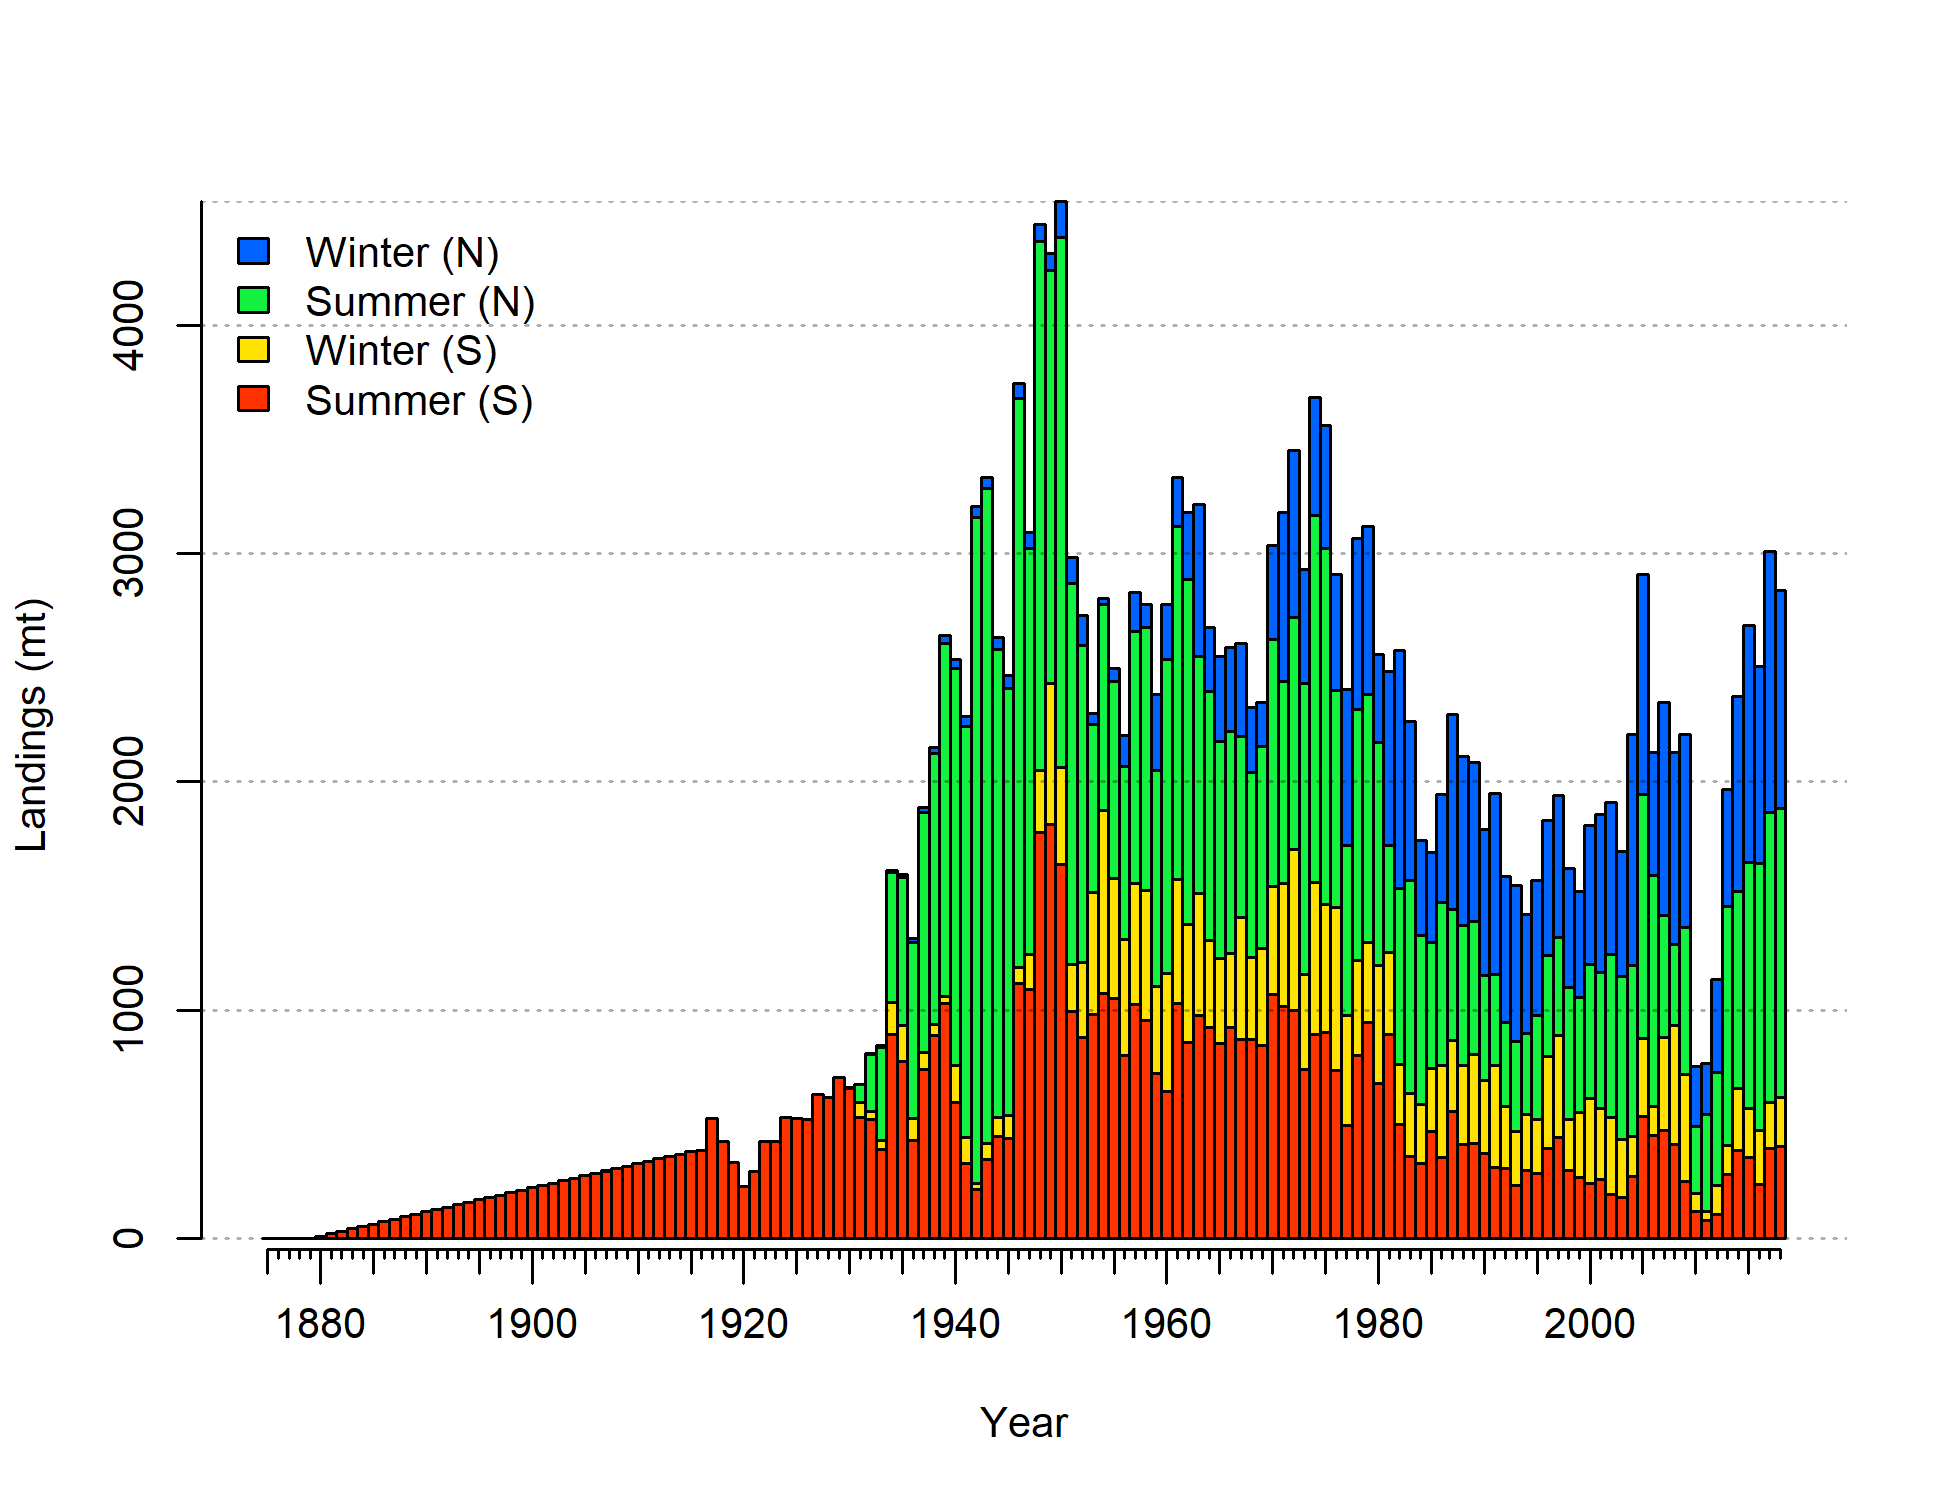
\includegraphics{r4ss/plots_mod1/catch2 landings stacked.png}
\caption{Total catches Petrale sole. \label{fig:Catch}}
\end{figure}

\FloatBarrier

\begin{figure}
\centering
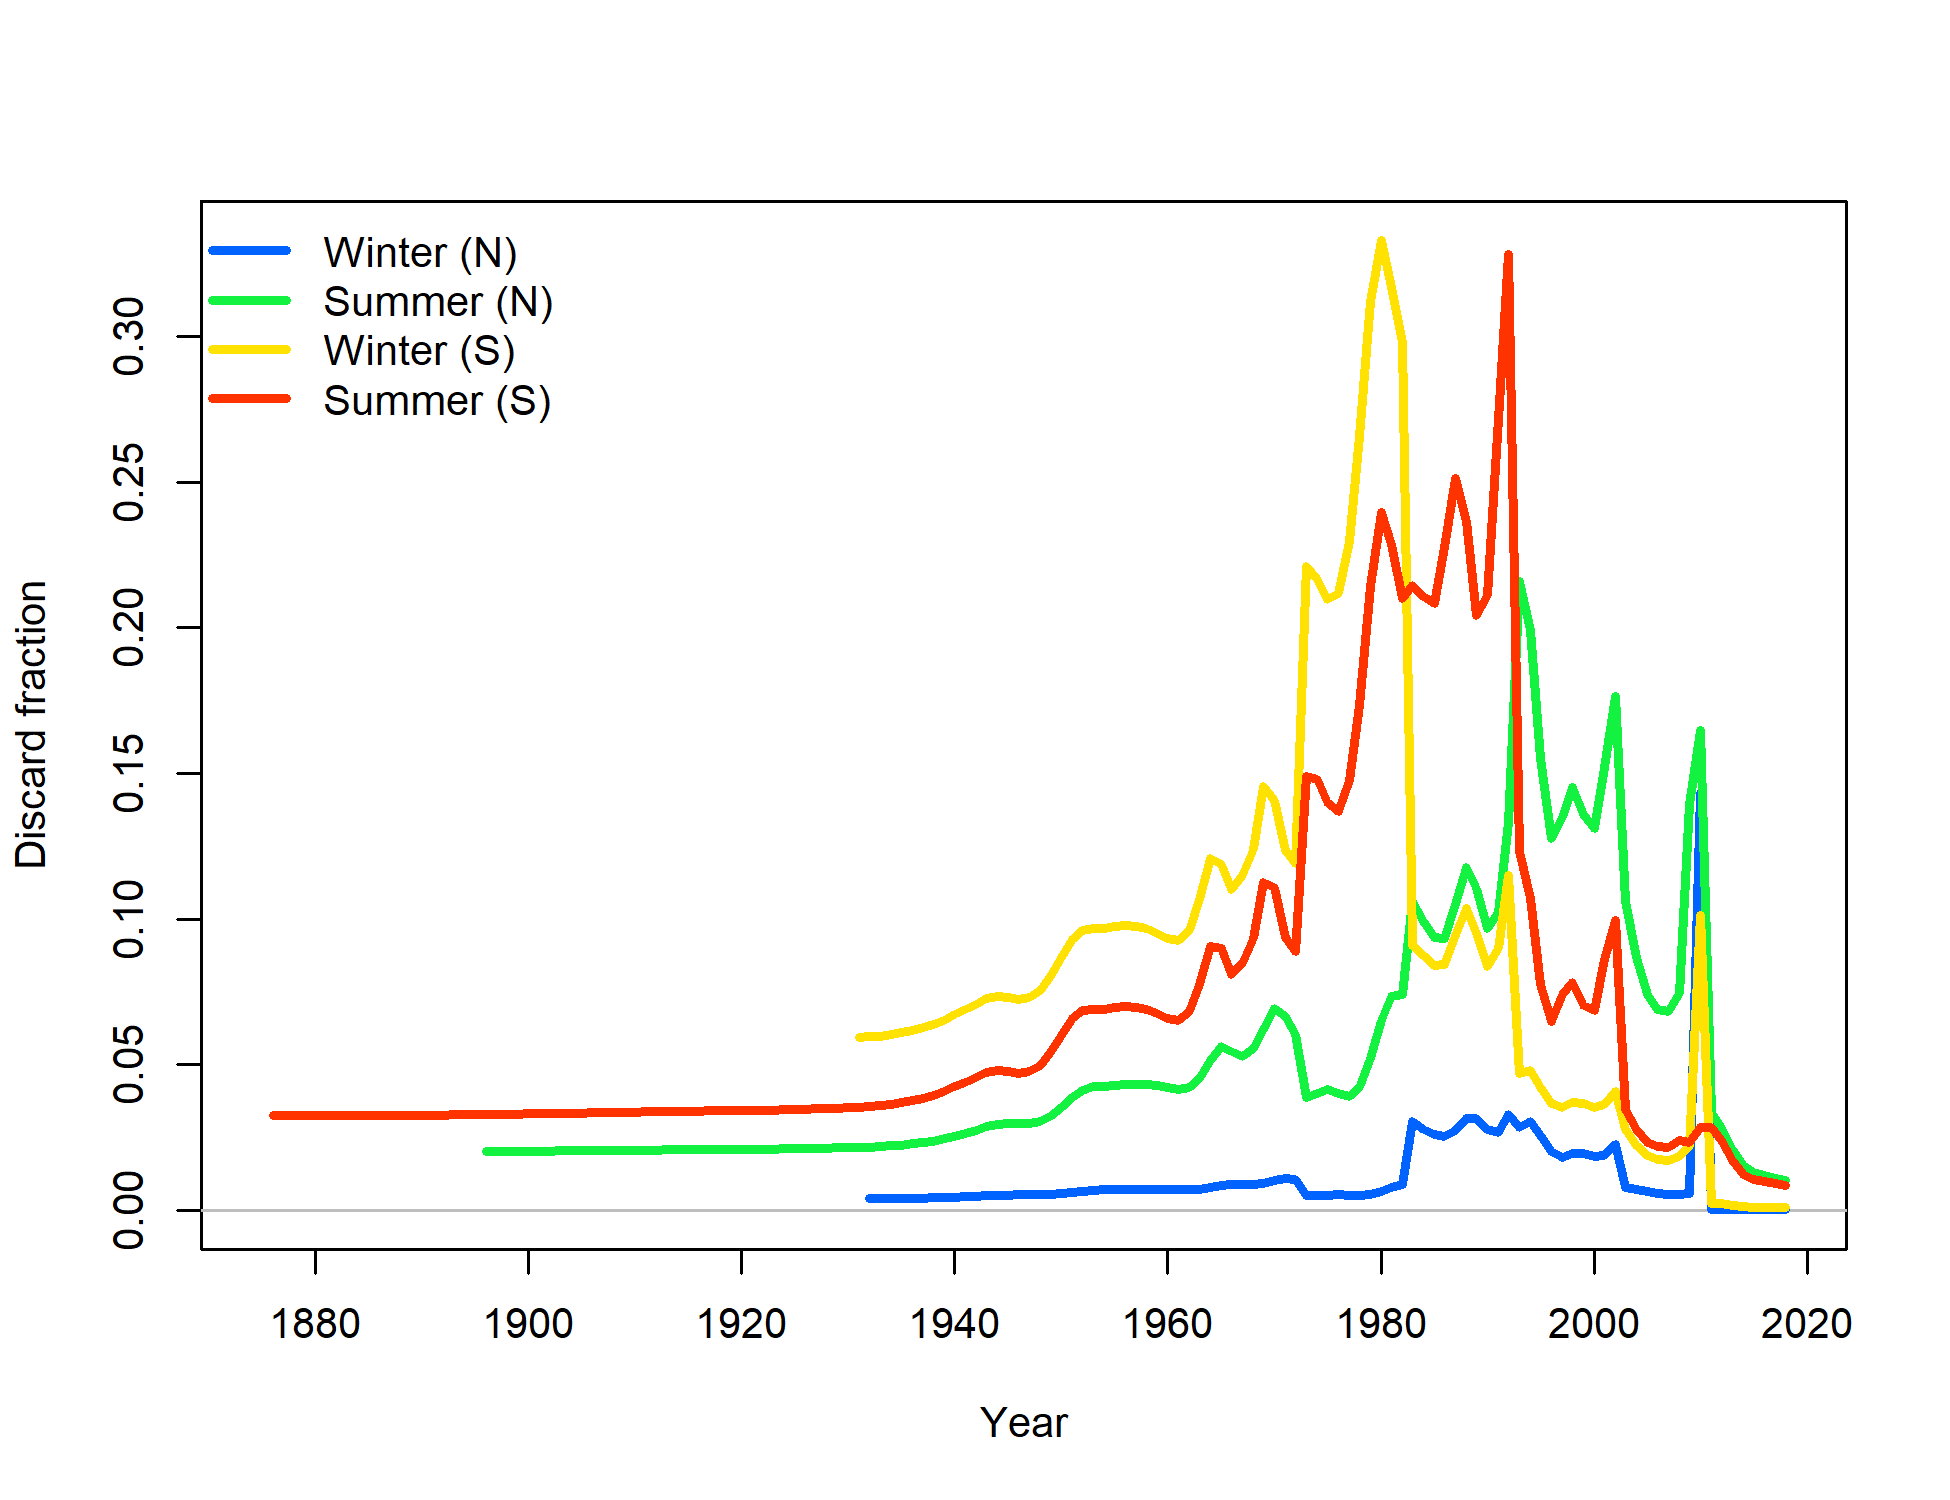
\includegraphics{r4ss/plots_mod1/catch8 discard fraction.png}
\caption{Discard rates by fleet for Petrale sole. \label{fig:Discard}}
\end{figure}

\FloatBarrier

\begin{figure}
\centering
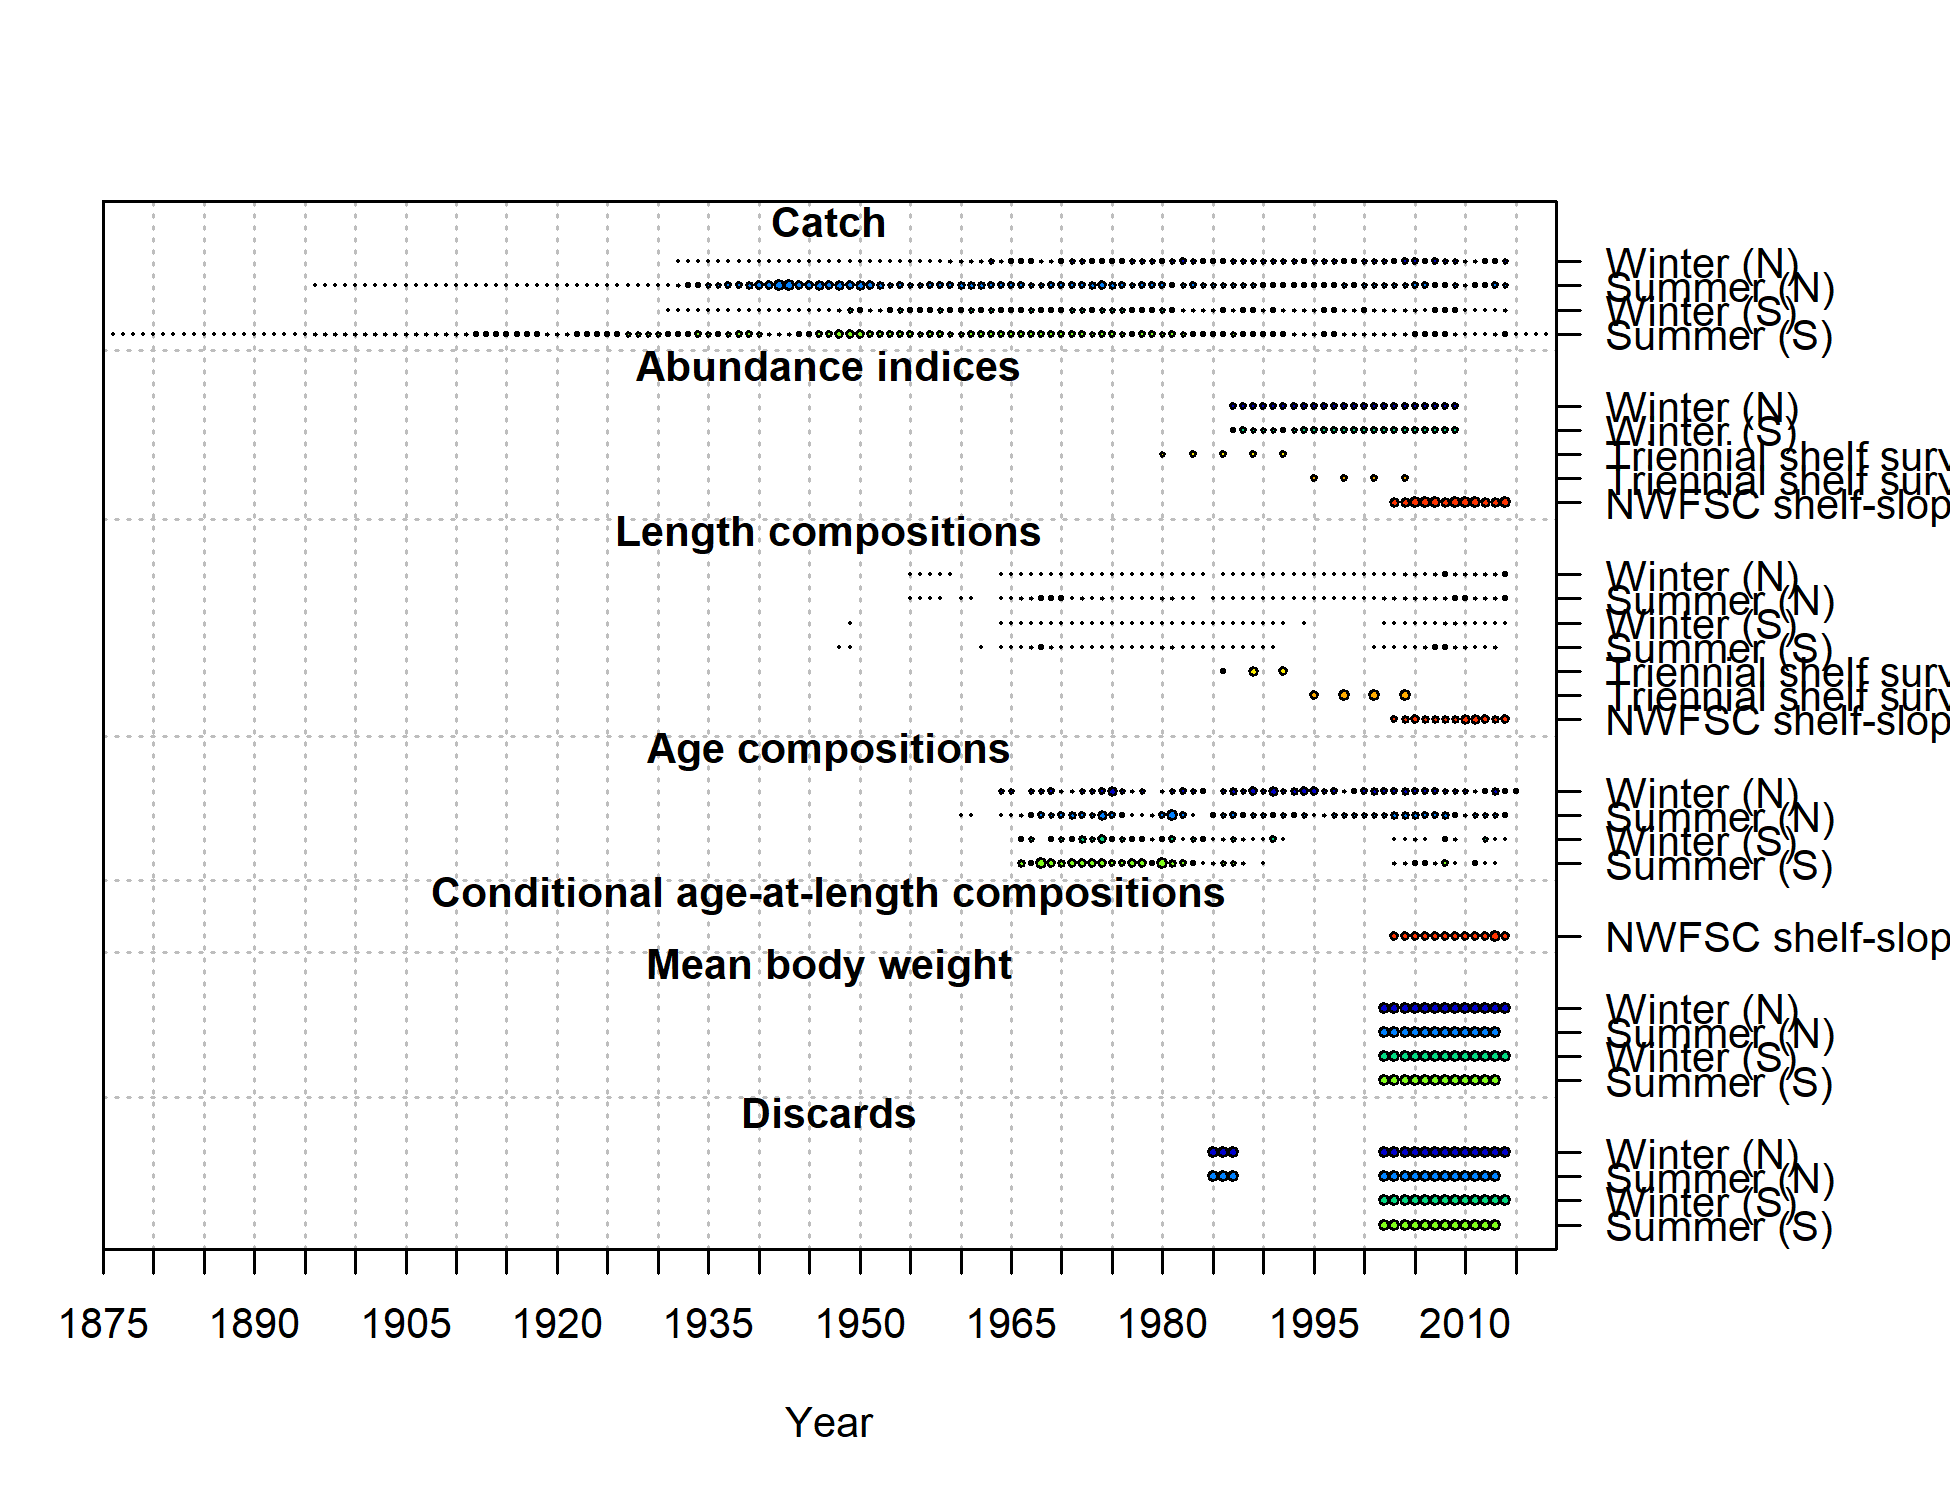
\includegraphics{r4ss/plots_mod1/data_plot2.png}
\caption{Summary of data sources used in the base model.
\label{fig:data_plot}}
\end{figure}

\FloatBarrier

\begin{figure}
\centering
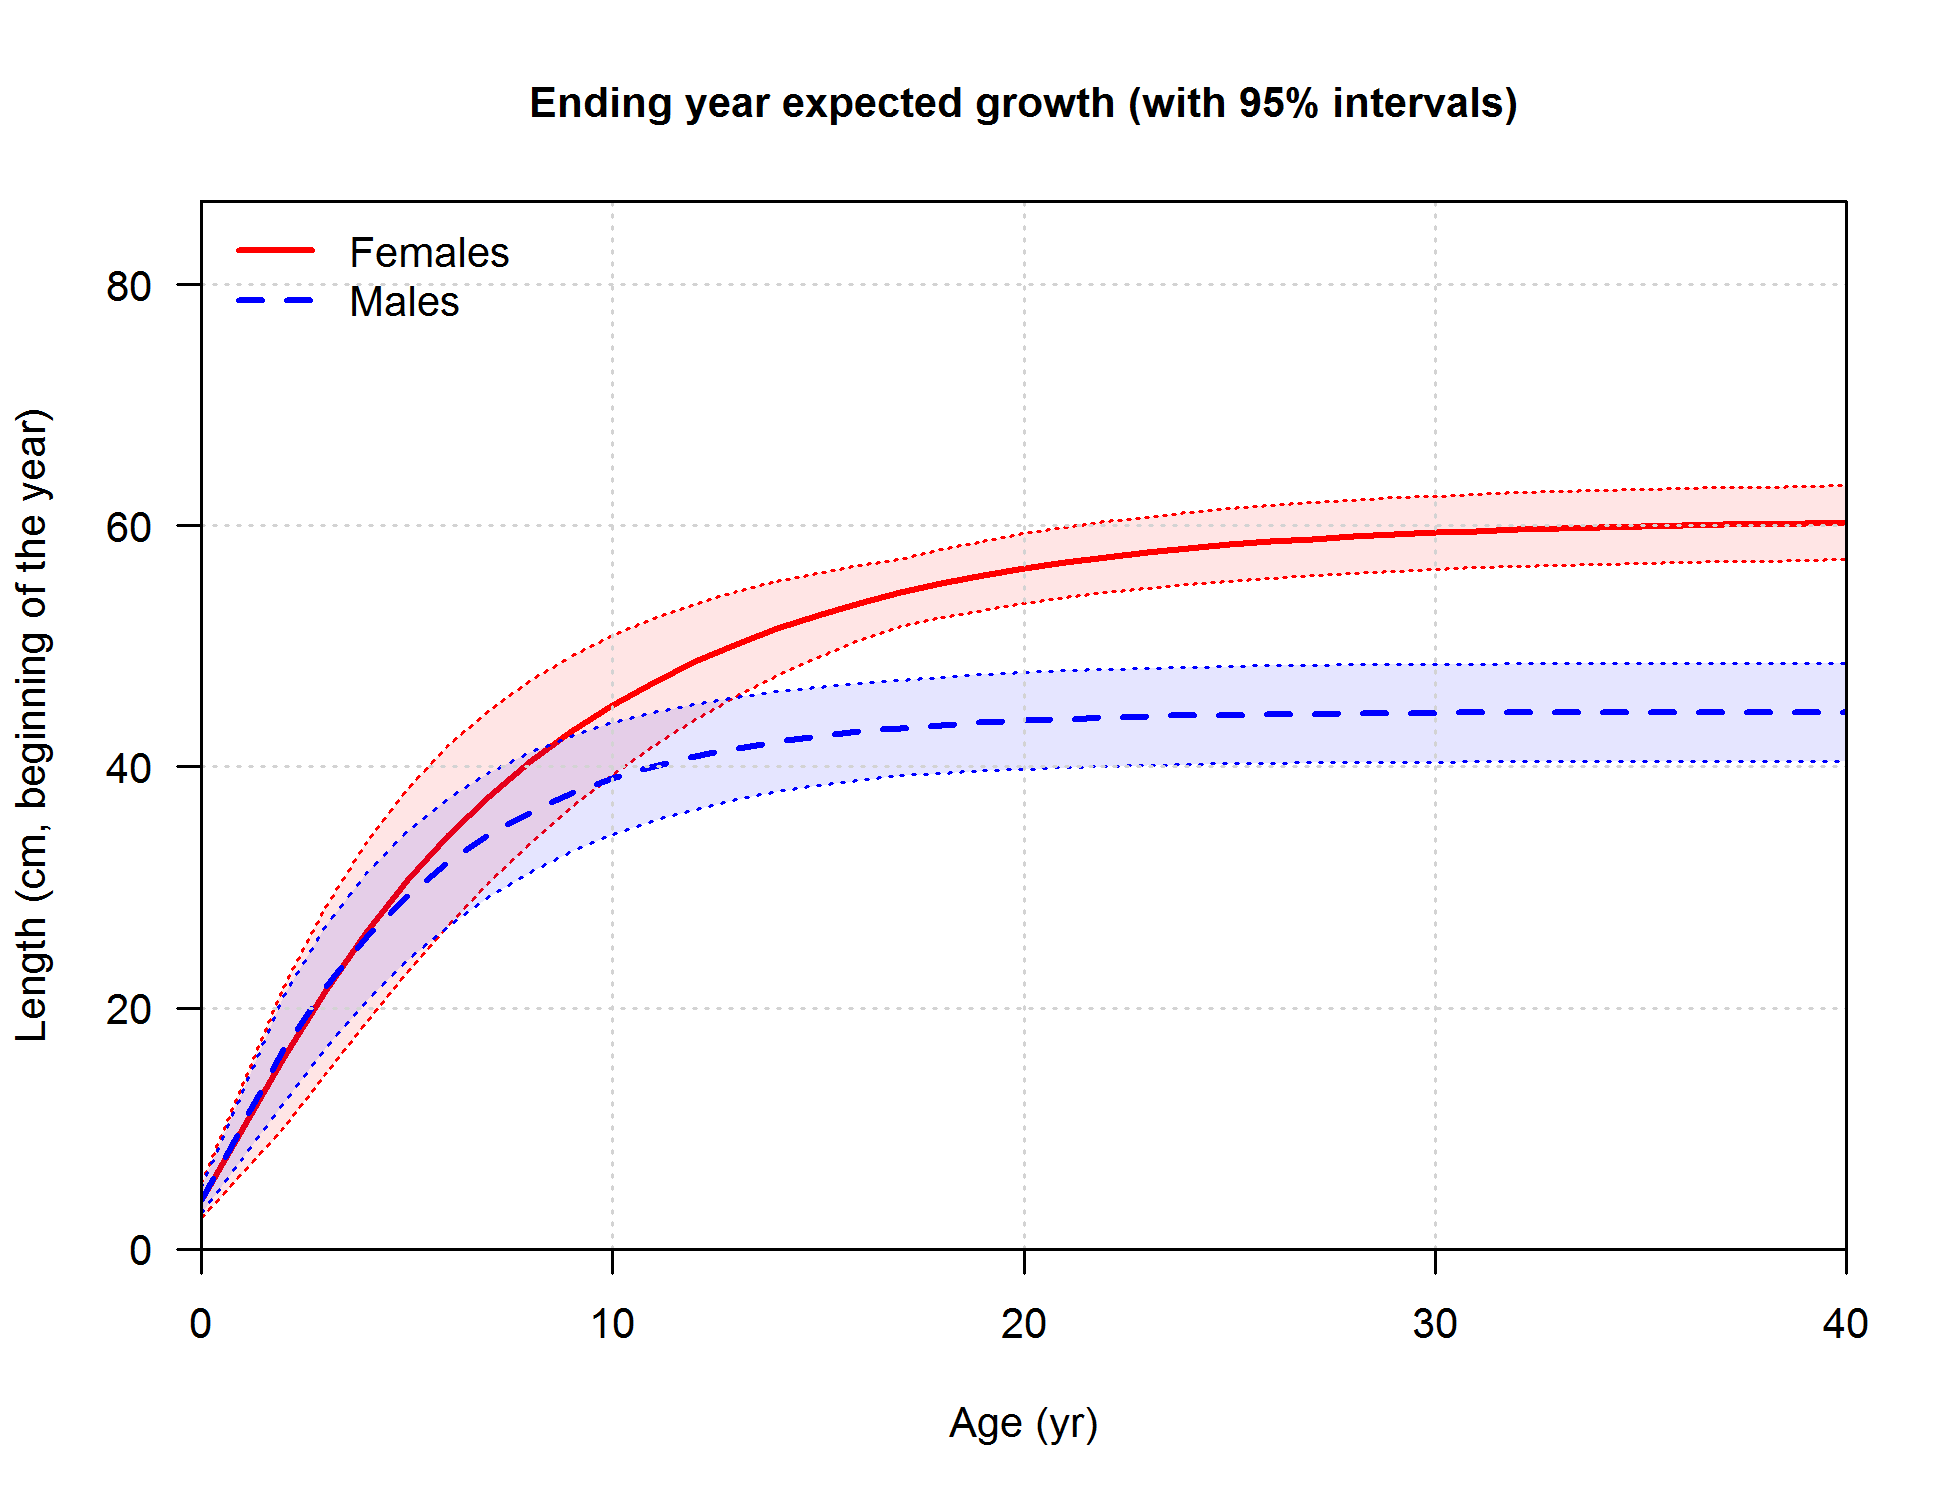
\includegraphics{r4ss/plots_mod1/bio1_sizeatage.png}
\caption{Estimated length-at-age for male and female for Petrale sole
with estimated CV. \label{fig:sizeatage}}
\end{figure}

\FloatBarrier 

\begin{figure}
\centering
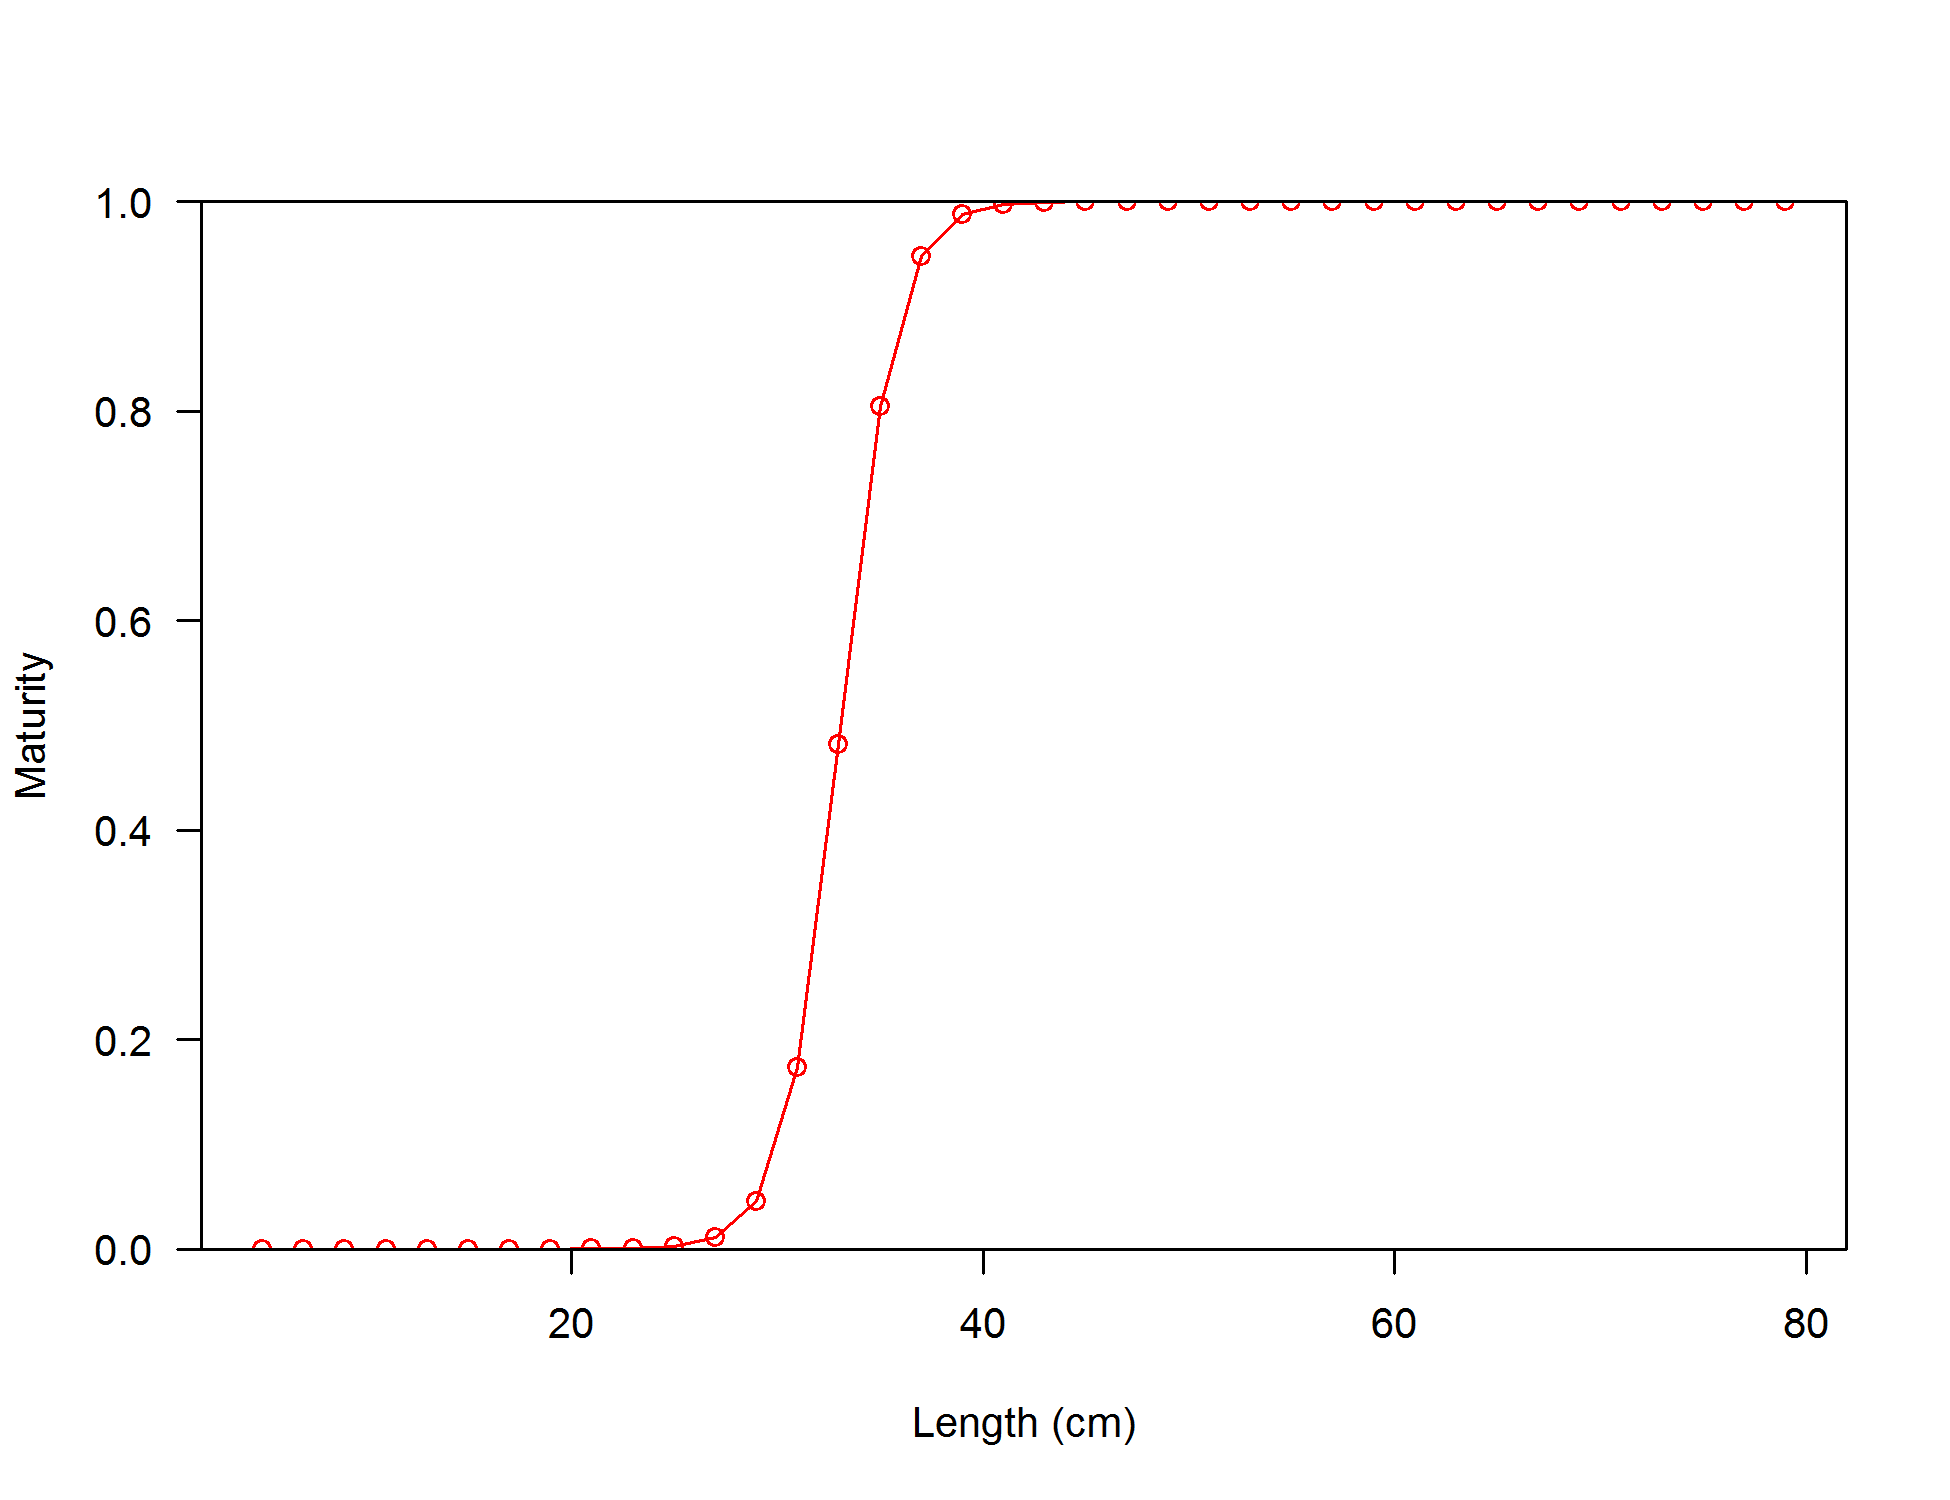
\includegraphics{r4ss/plots_mod1/bio6_maturity.png}
\caption{Estimated maturity-at-length for Petrale sole.
\label{fig:maturity}}
\end{figure}

\FloatBarrier

\begin{figure}
\centering
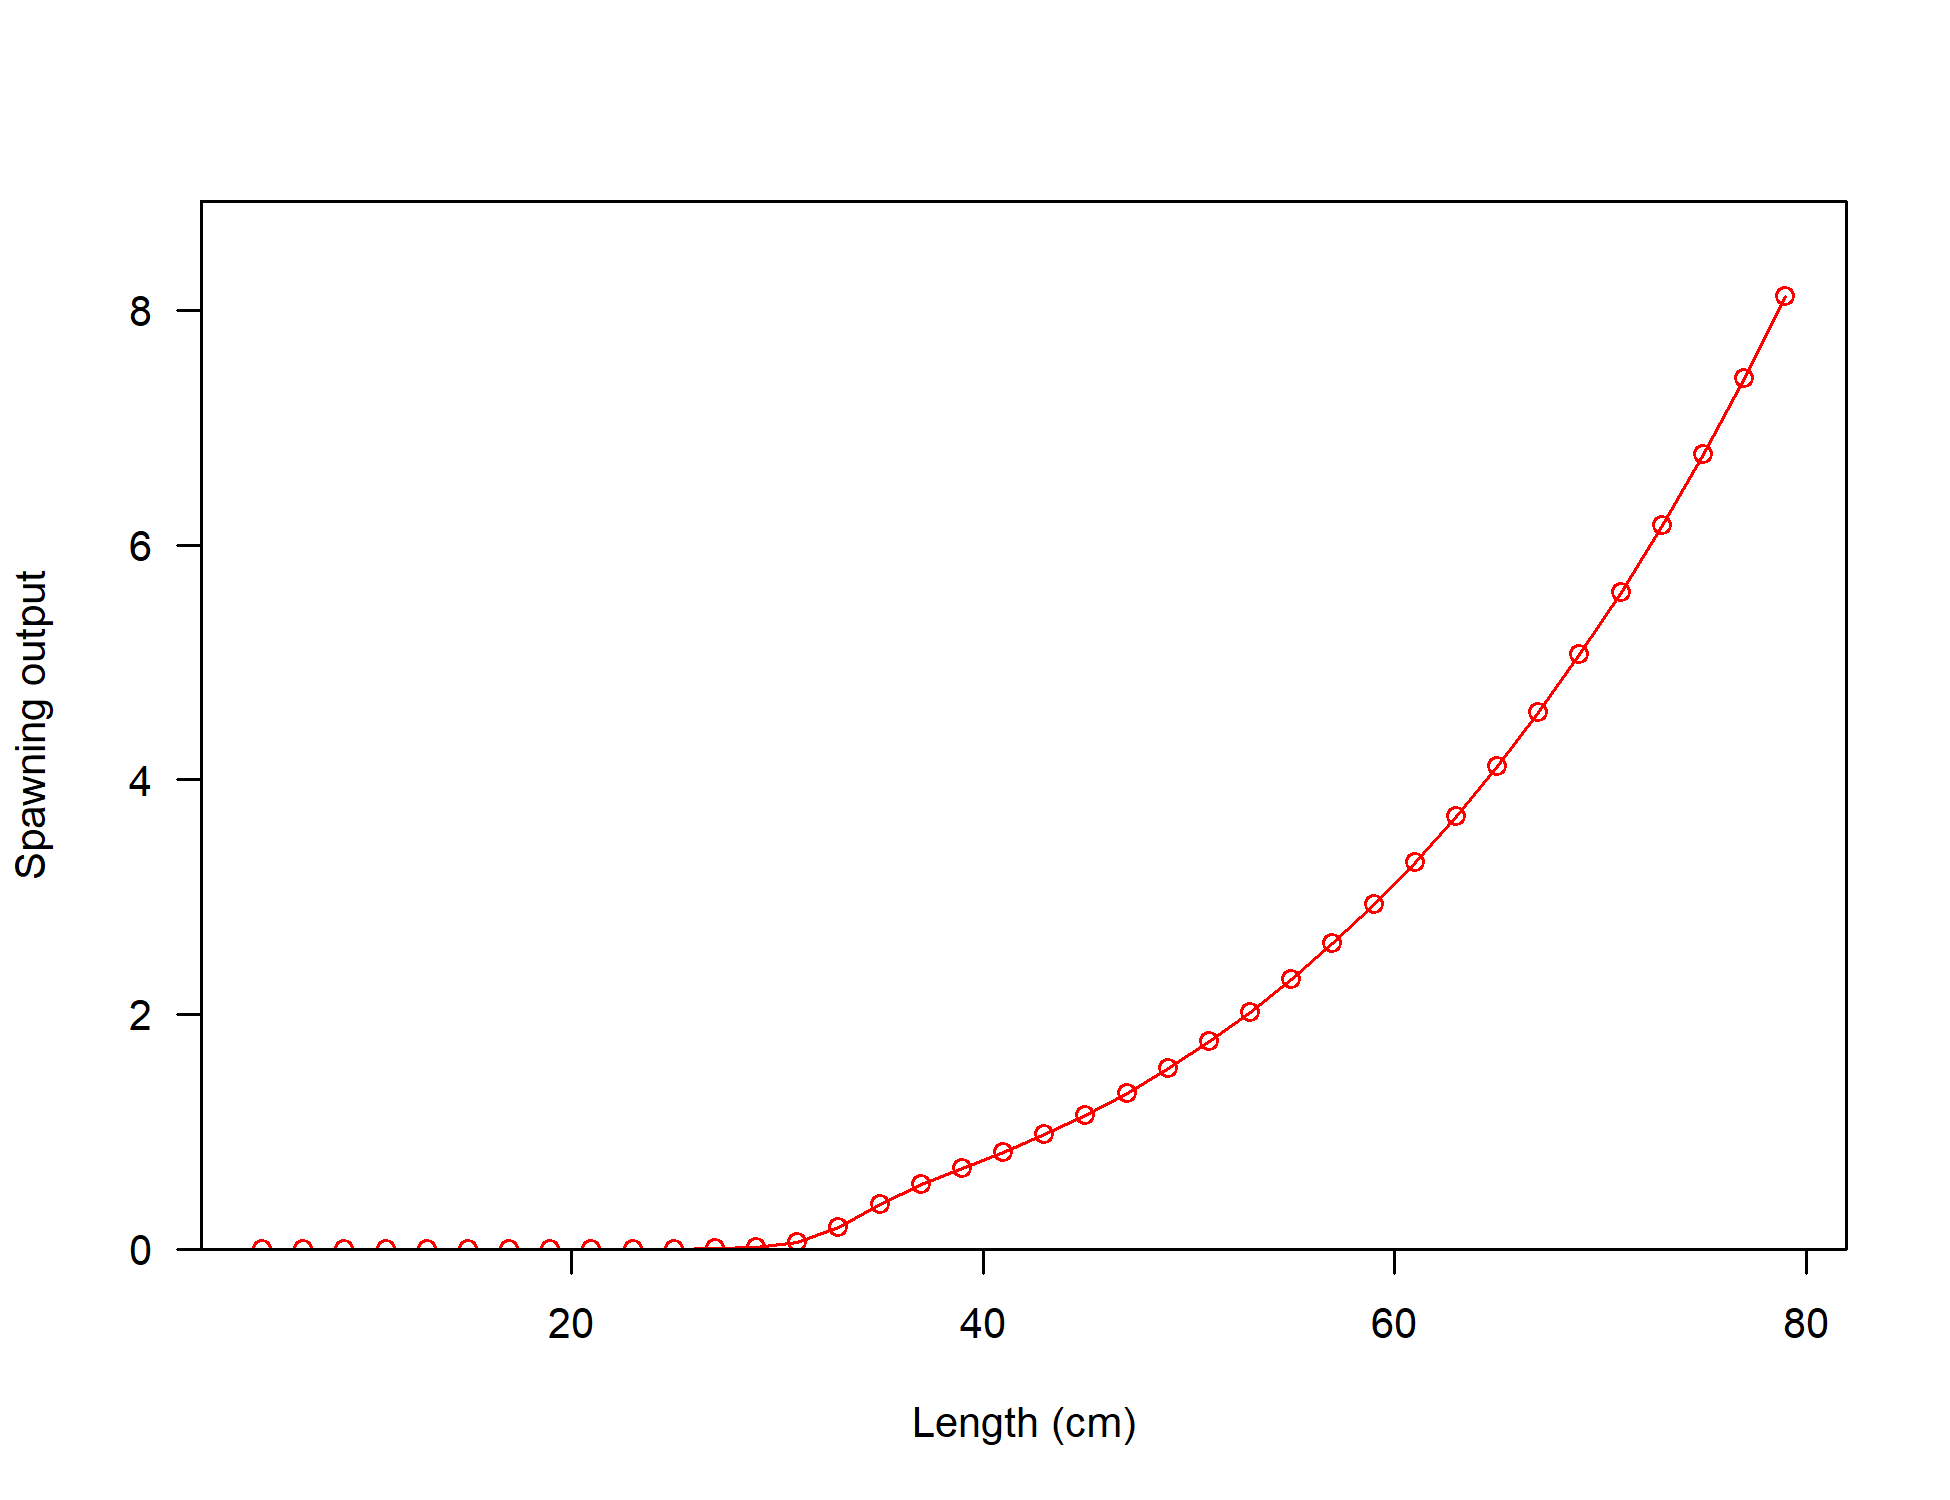
\includegraphics{r4ss/plots_mod1/bio10_spawningoutput_len.png}
\caption{Estimated spawning output-at-length for female Petrale sole.
\label{fig:spawnoutlen}}
\end{figure}

\FloatBarrier 

\begin{figure}
\centering
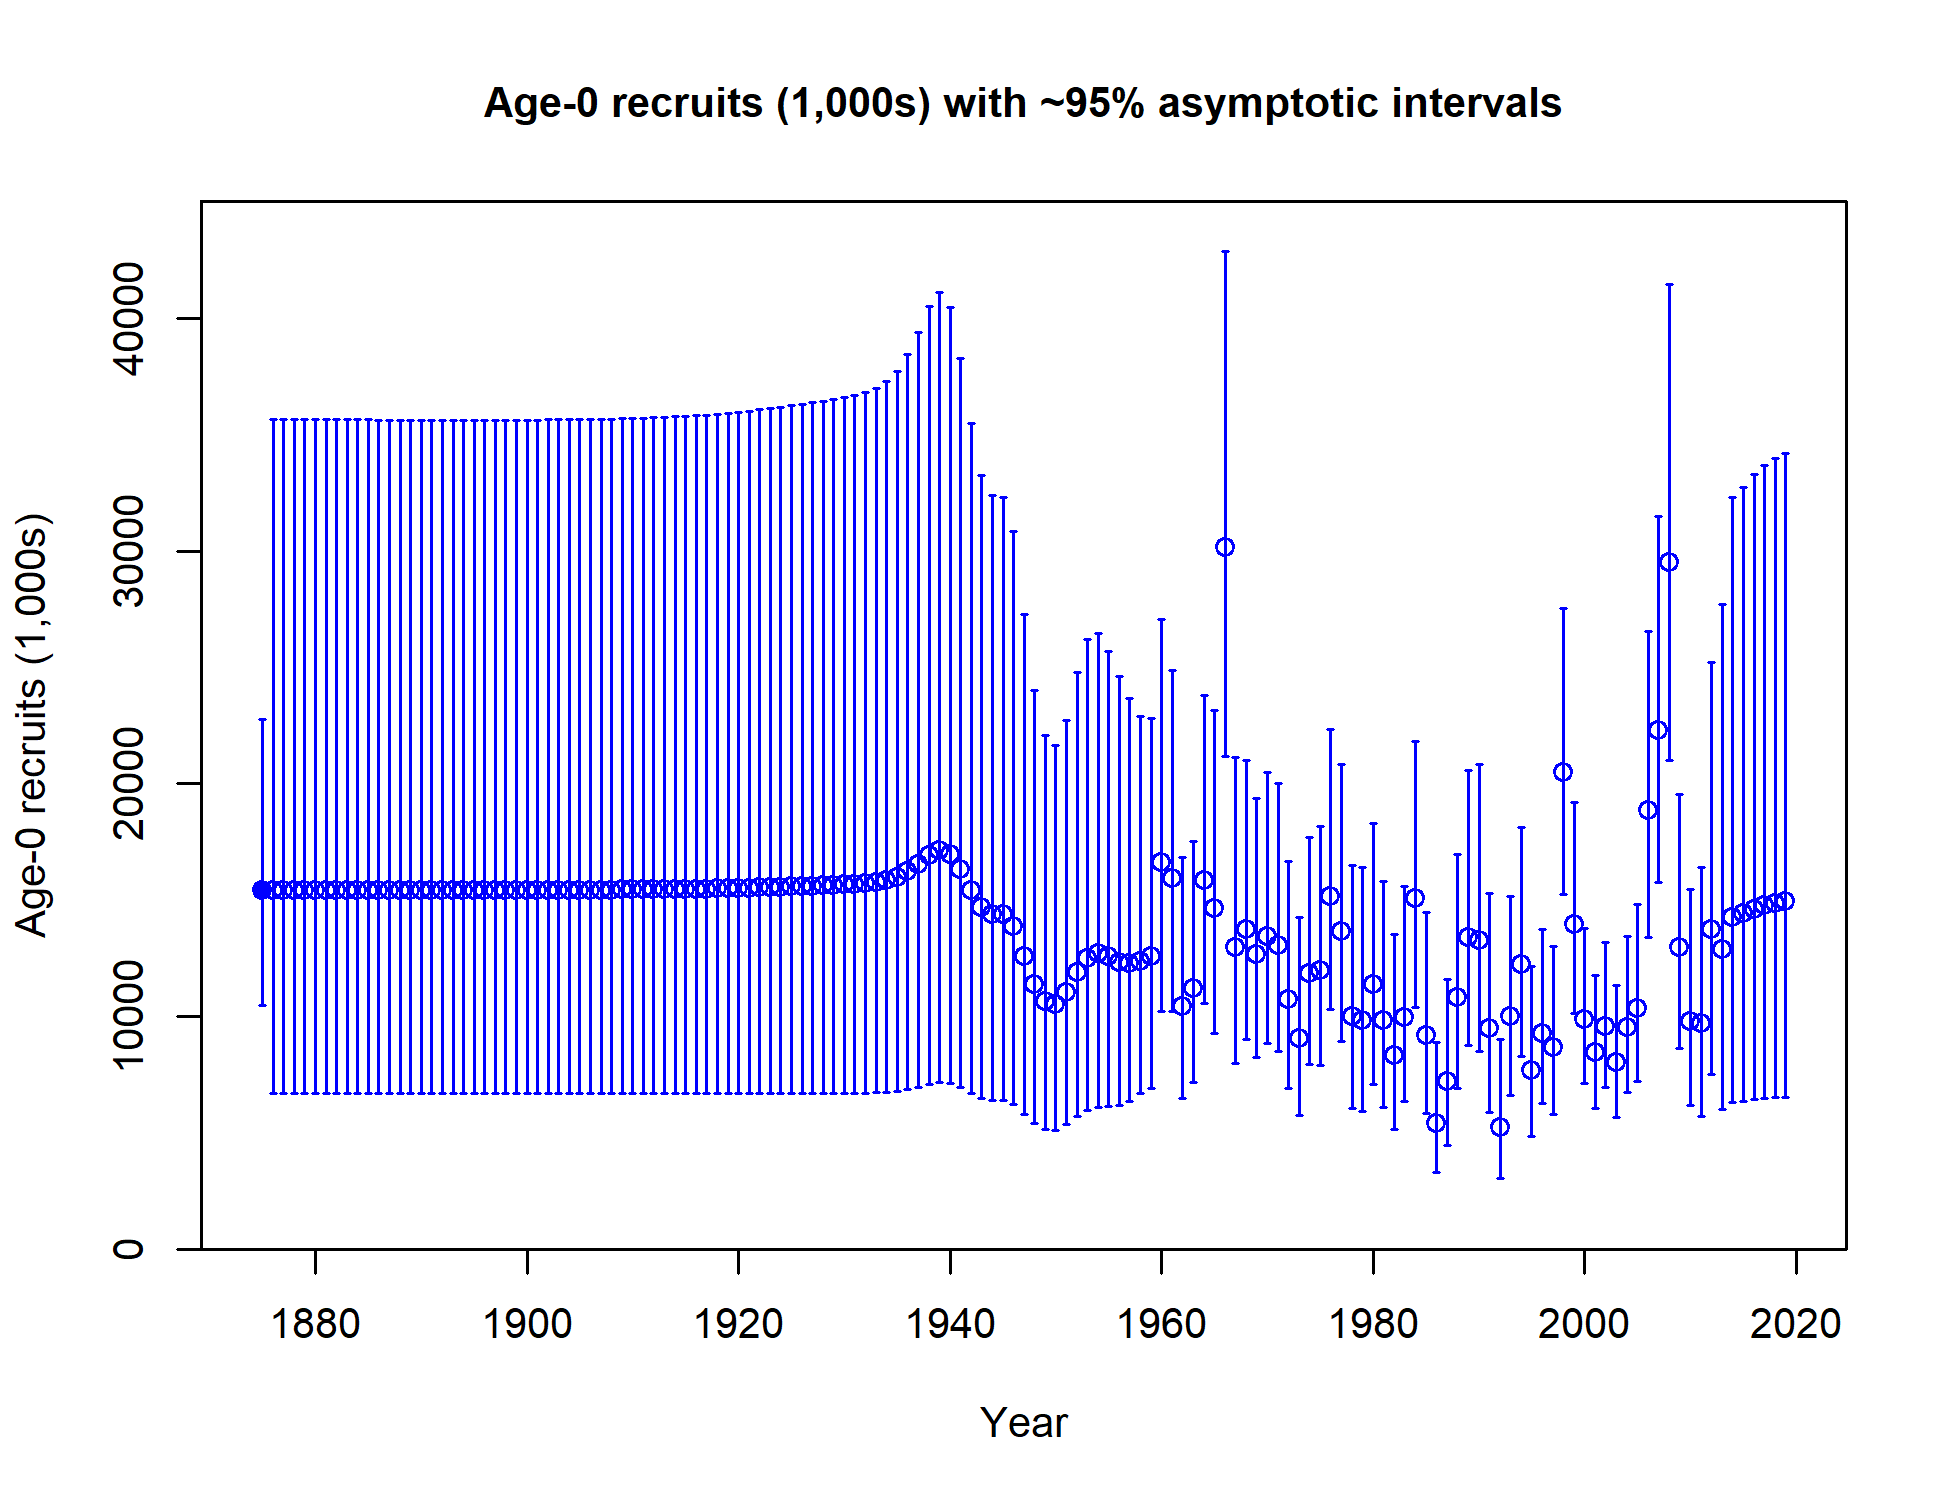
\includegraphics{r4ss/plots_mod1/ts11_Age-0_recruits_(1000s)_with_95_asymptotic_intervals.png}
\caption{Estimated time-series of recruitment for Petrale sole.
\label{fig:recruits}}
\end{figure}

\FloatBarrier

\begin{figure}
\centering
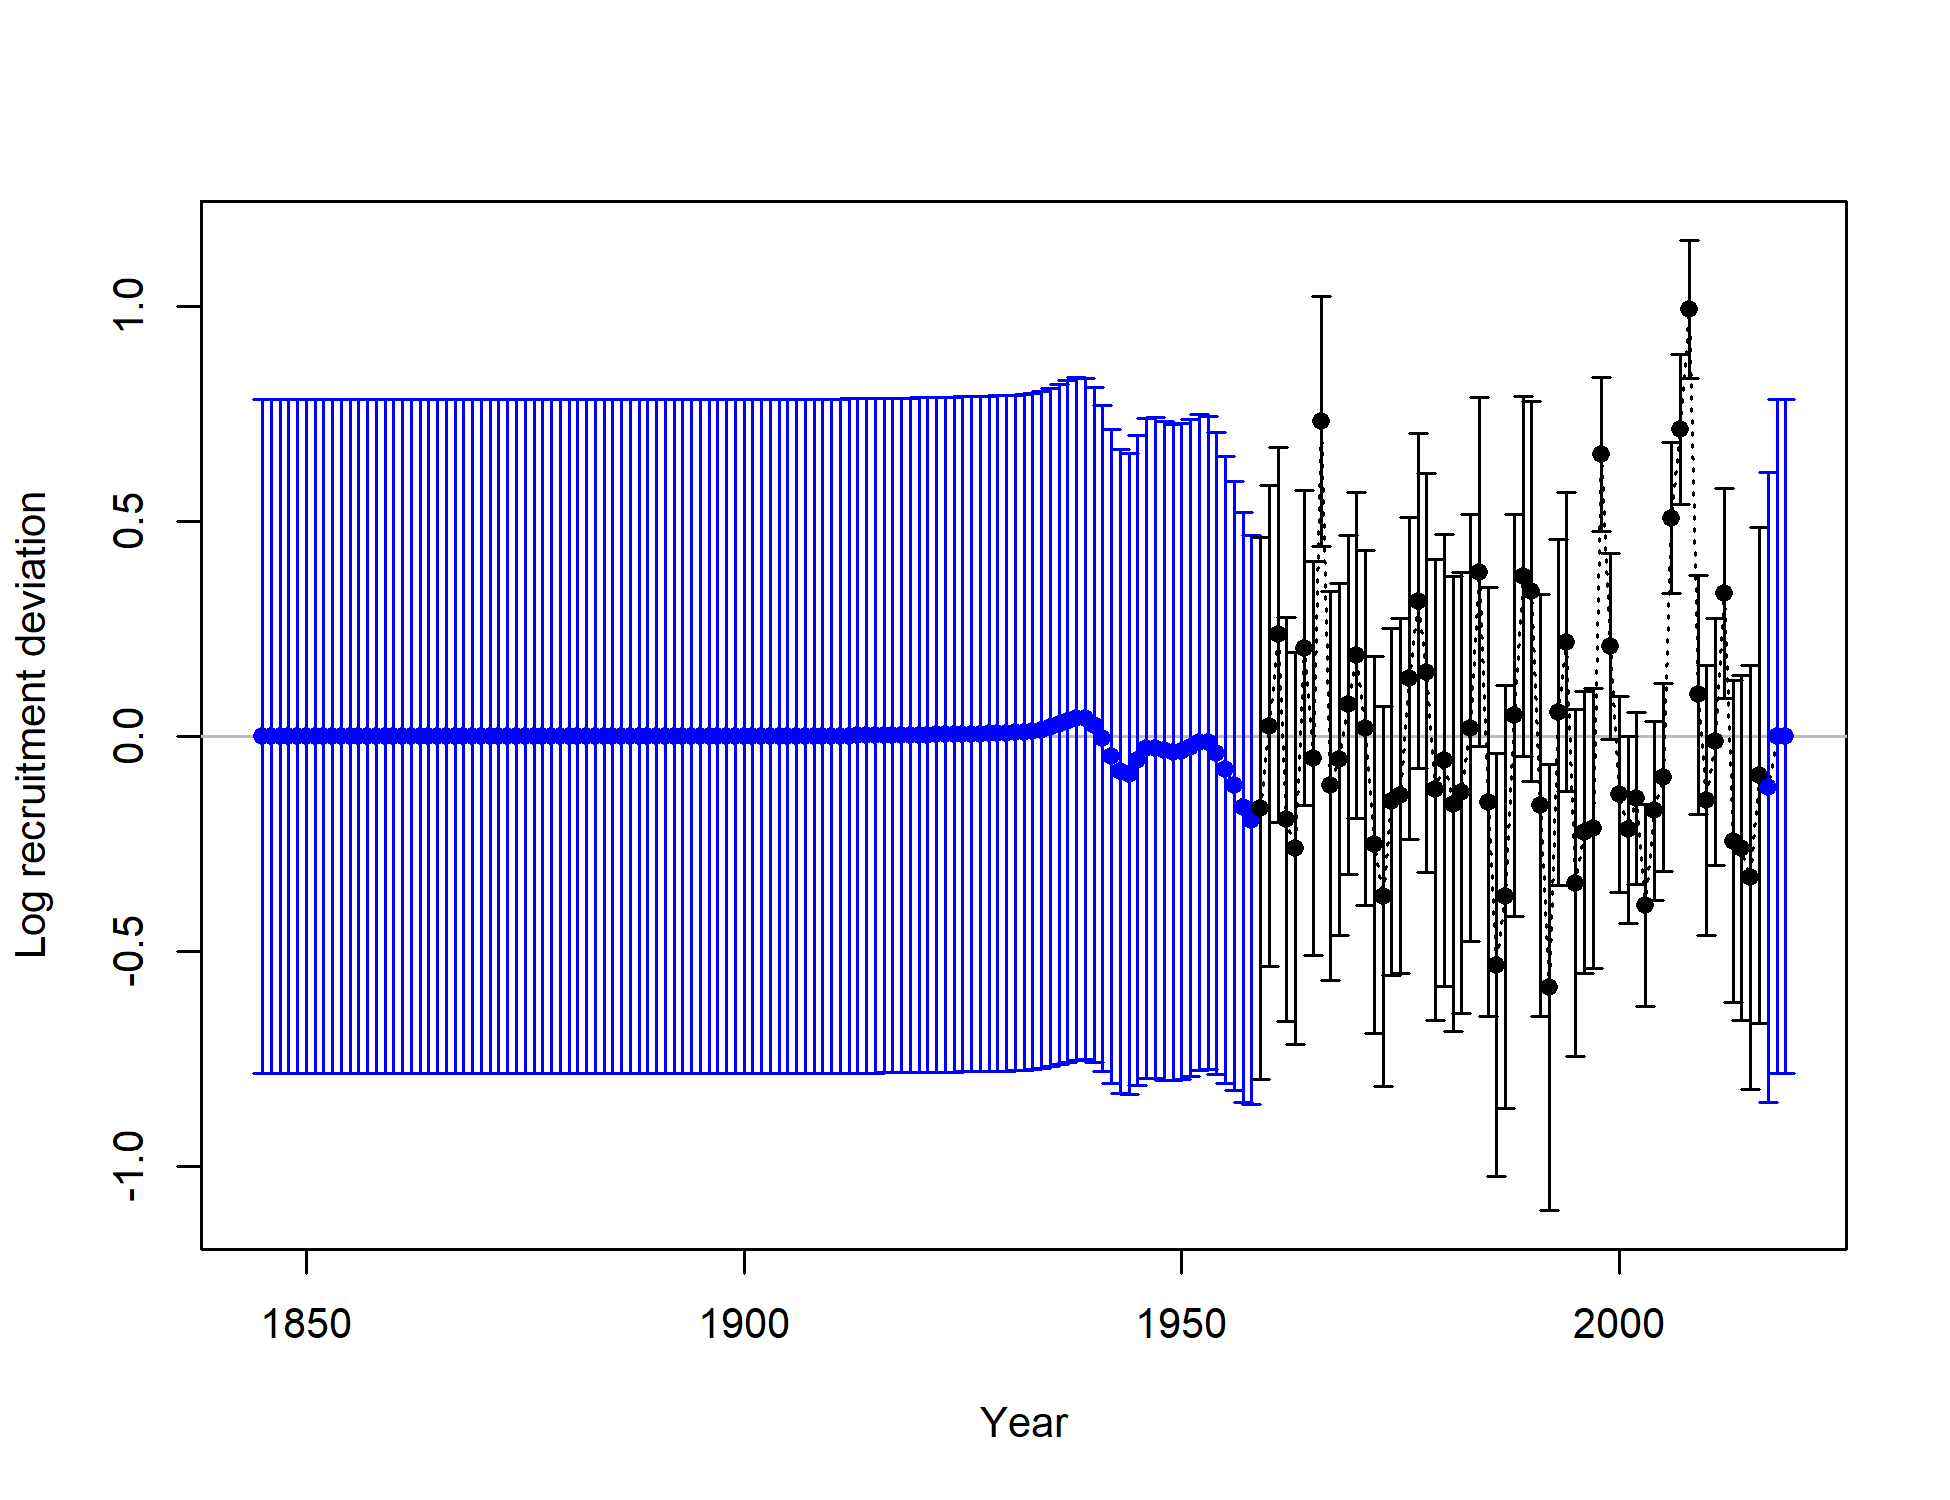
\includegraphics{r4ss/plots_mod1/recdevs2_withbars.png}
\caption{Estimated time-series of recruitment deviations for Petrale
sole. \label{fig:recdevs}}
\end{figure}

\FloatBarrier

\begin{figure}
\centering
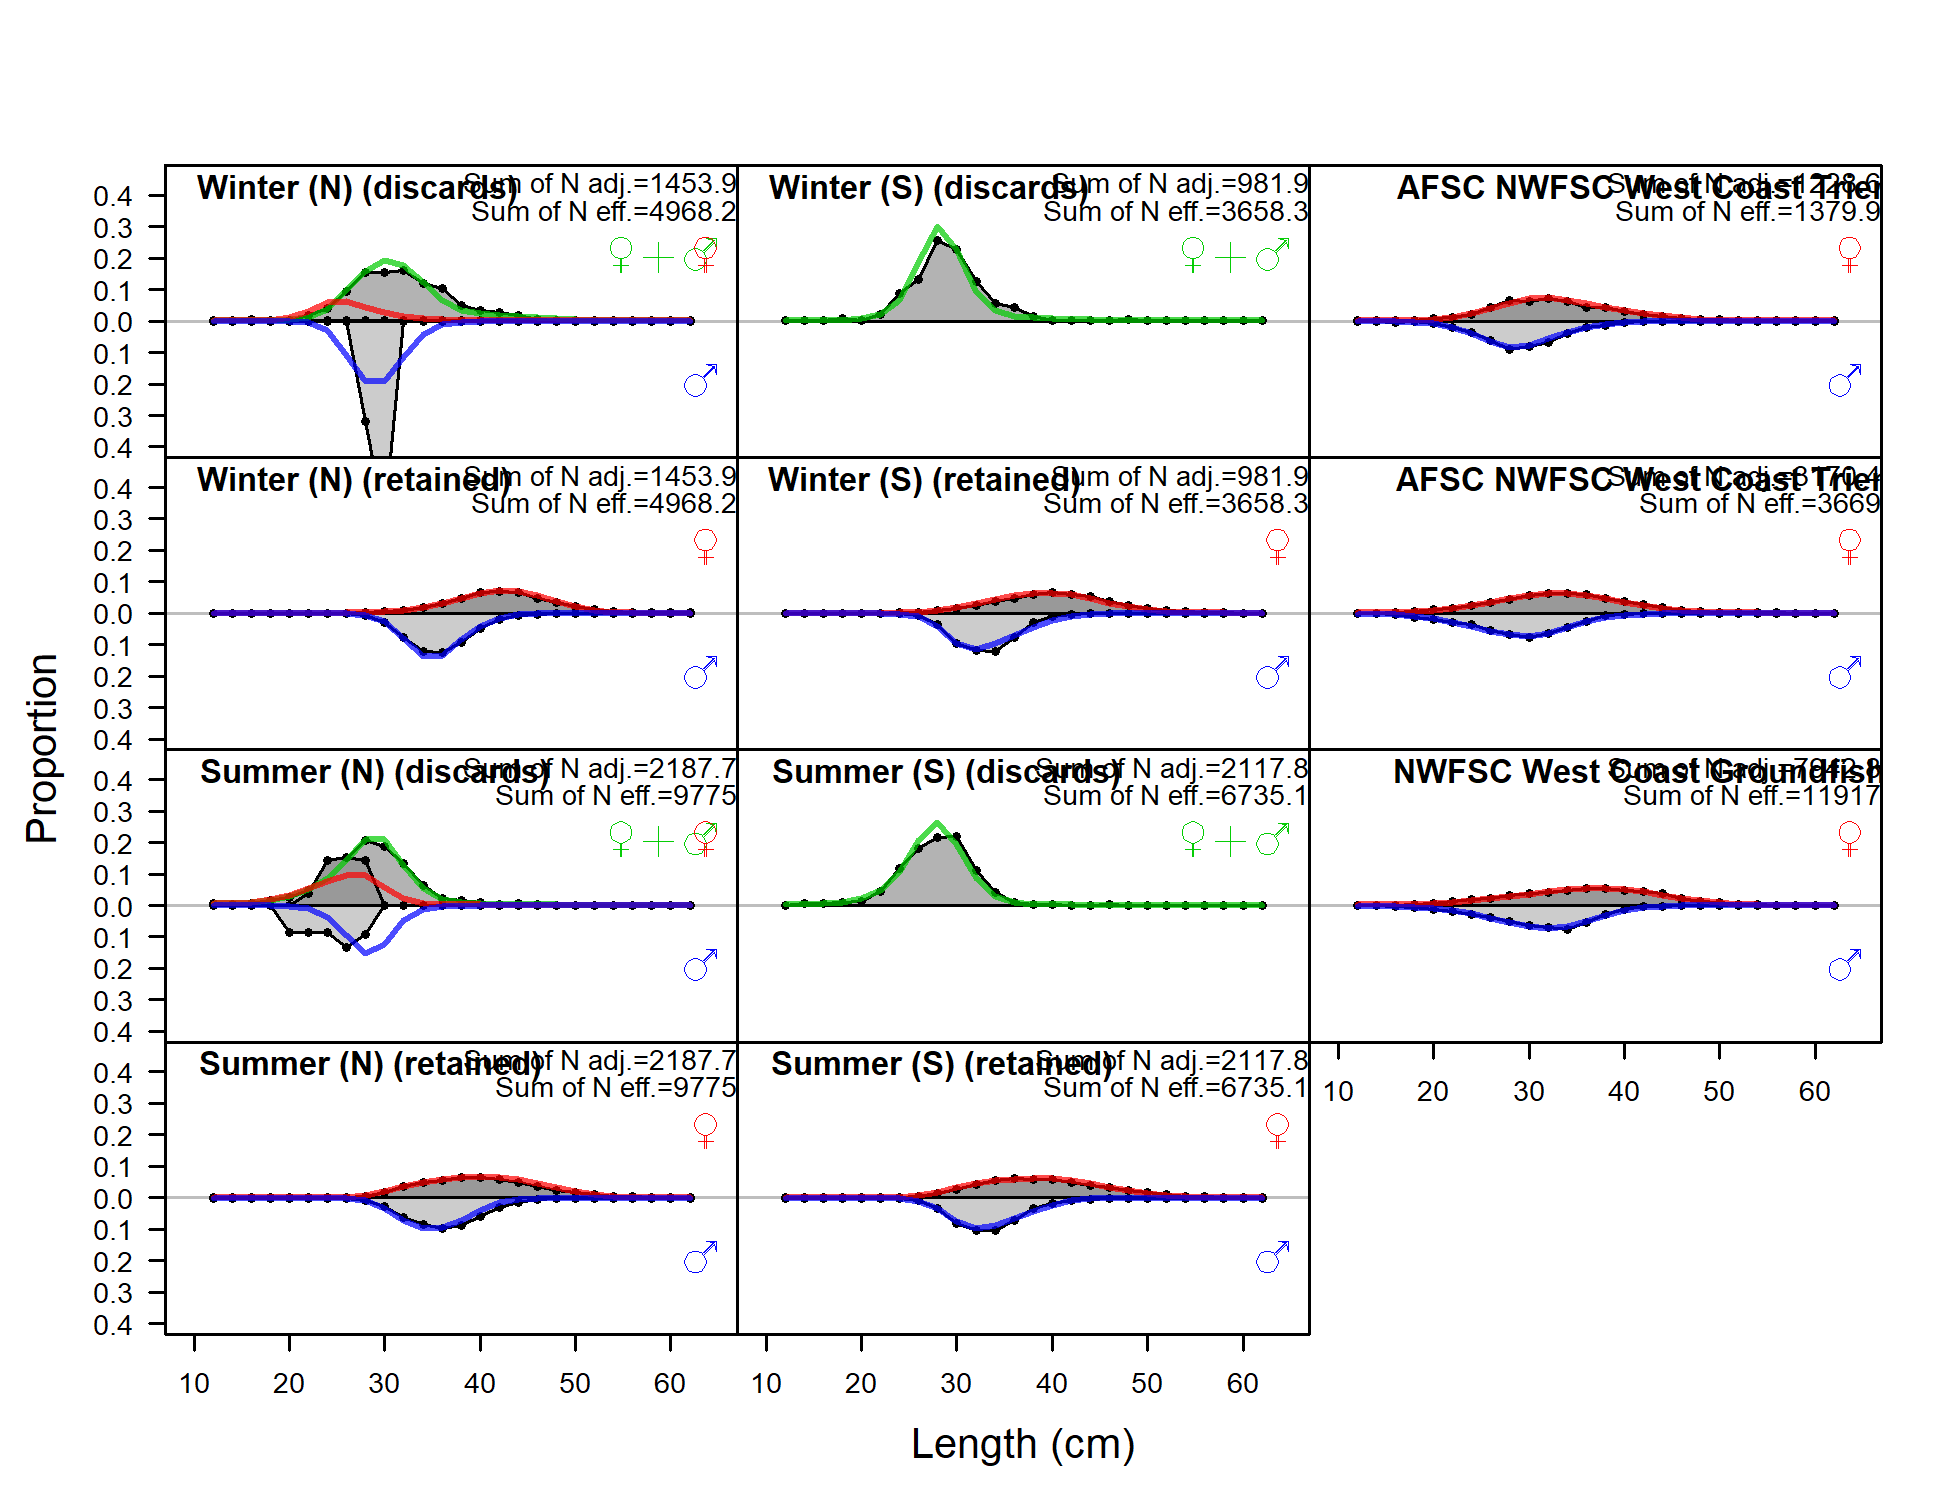
\includegraphics{r4ss/plots_mod1/comp_lenfit__aggregated_across_time.png}
\caption{Length compositions aggregated across time by fleet. Labels
`retained' and `discard' indicate retained or discarded samples for each
fleet. Panels without this designation represent the whole catch. The
Triennial shelf survey length data were not used in the final model, but
the implied model fits are shown. \label{fig:length_agg}}
\end{figure}

\FloatBarrier

\begin{figure}
\centering
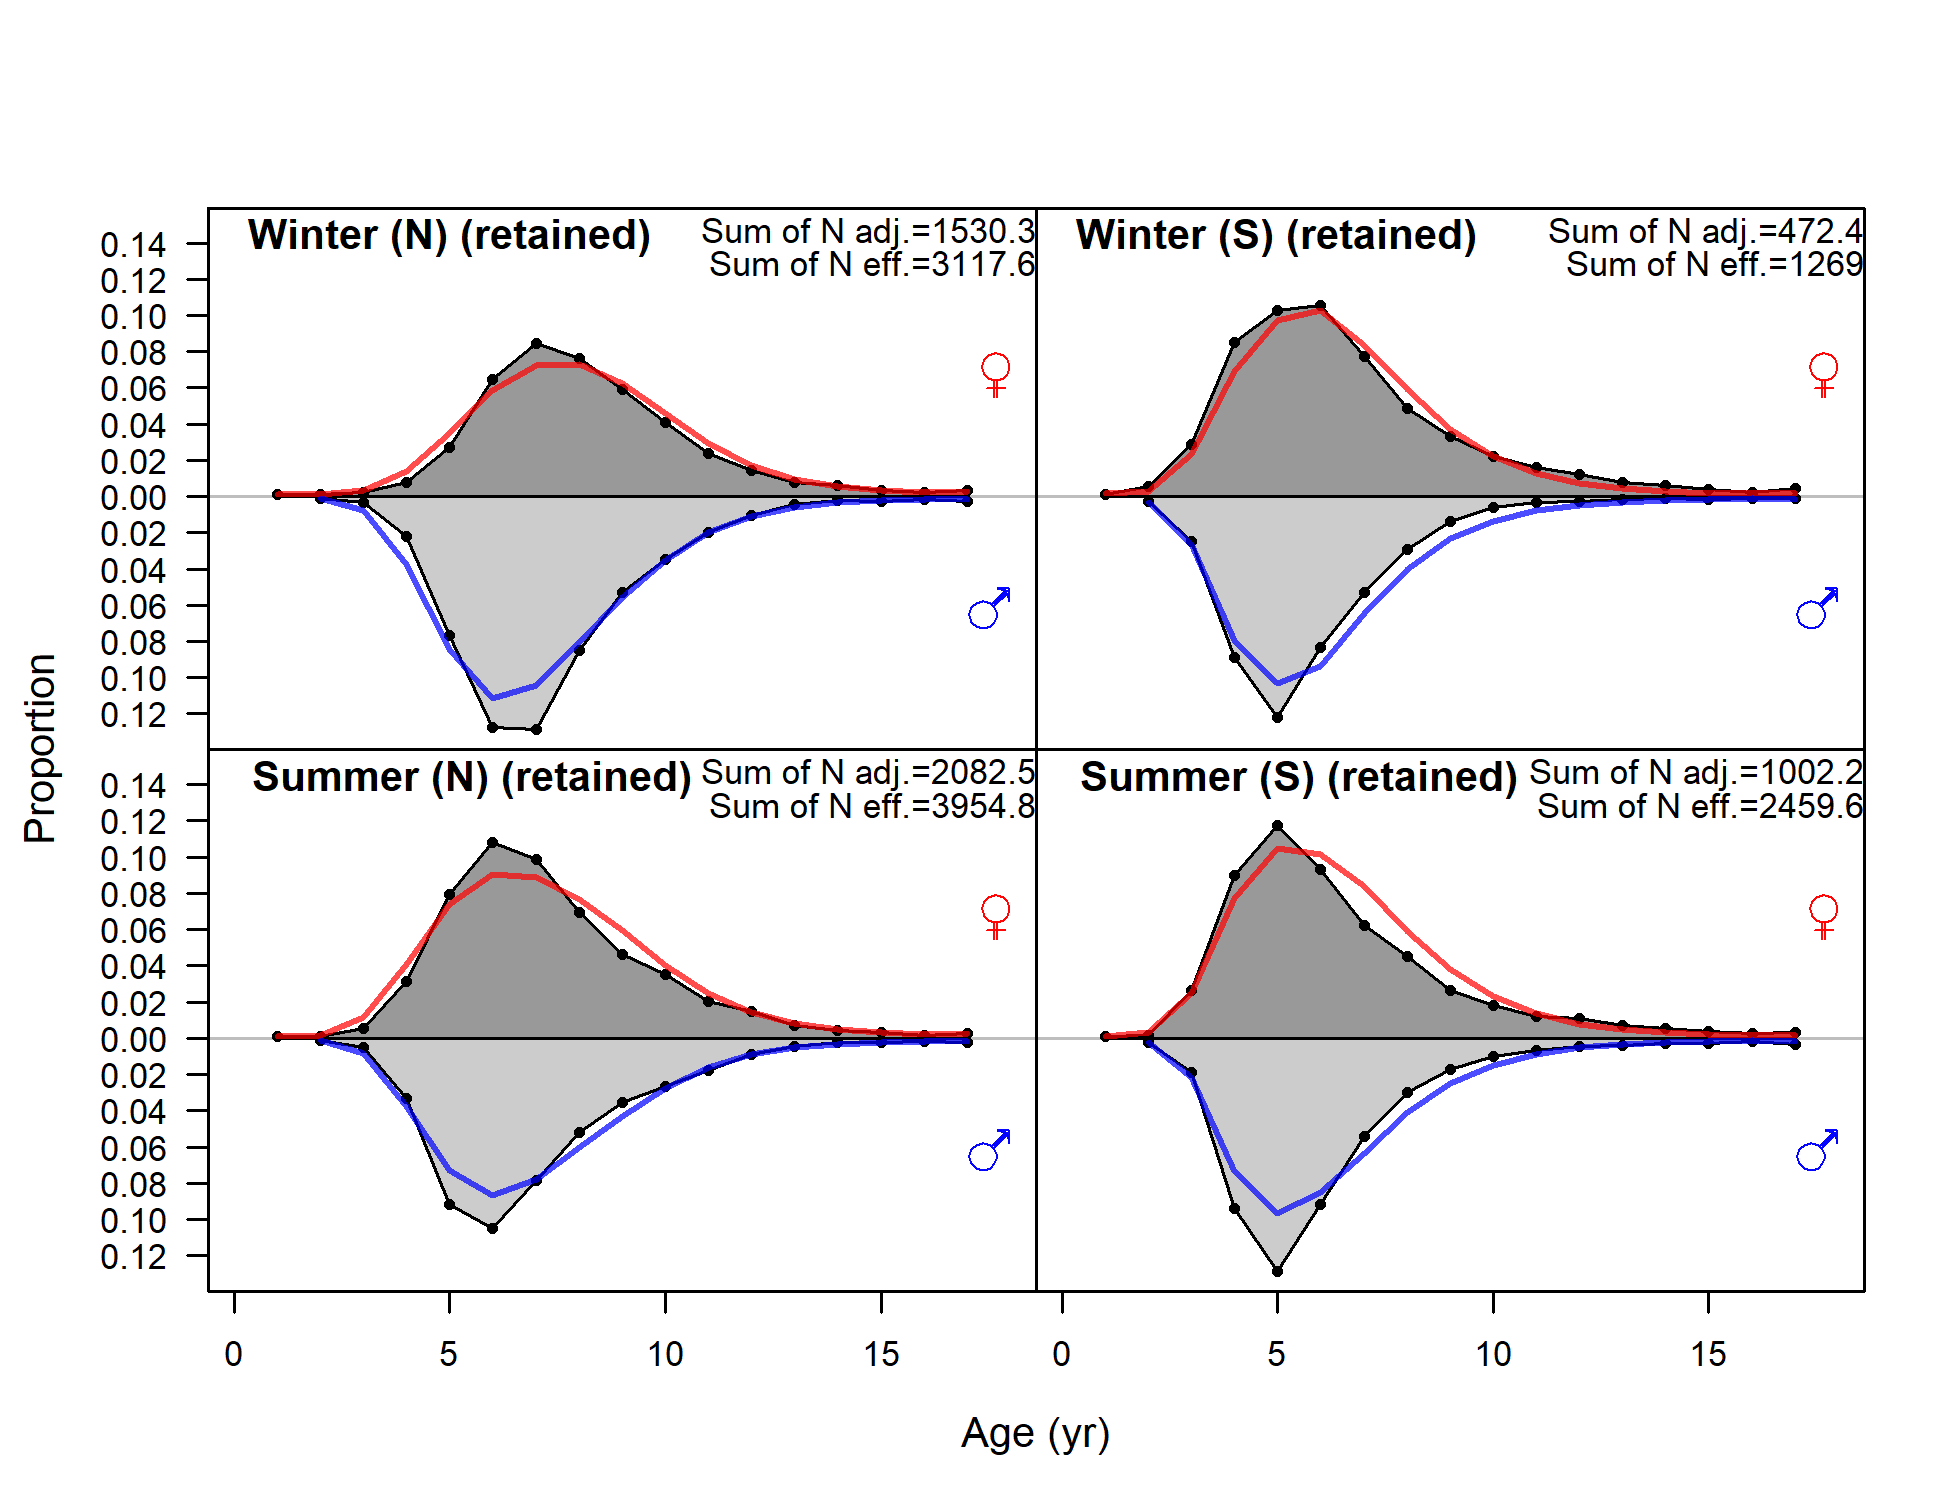
\includegraphics{r4ss/plots_mod1/comp_agefit__aggregated_across_time.png}
\caption{Age compositions aggregated across time by fleet. The Triennial
shelf survey age data were not used in the final model, but the implied
model fits are shown. \label{fig:age_agg}}
\end{figure}

\FloatBarrier

\begin{figure}
\centering
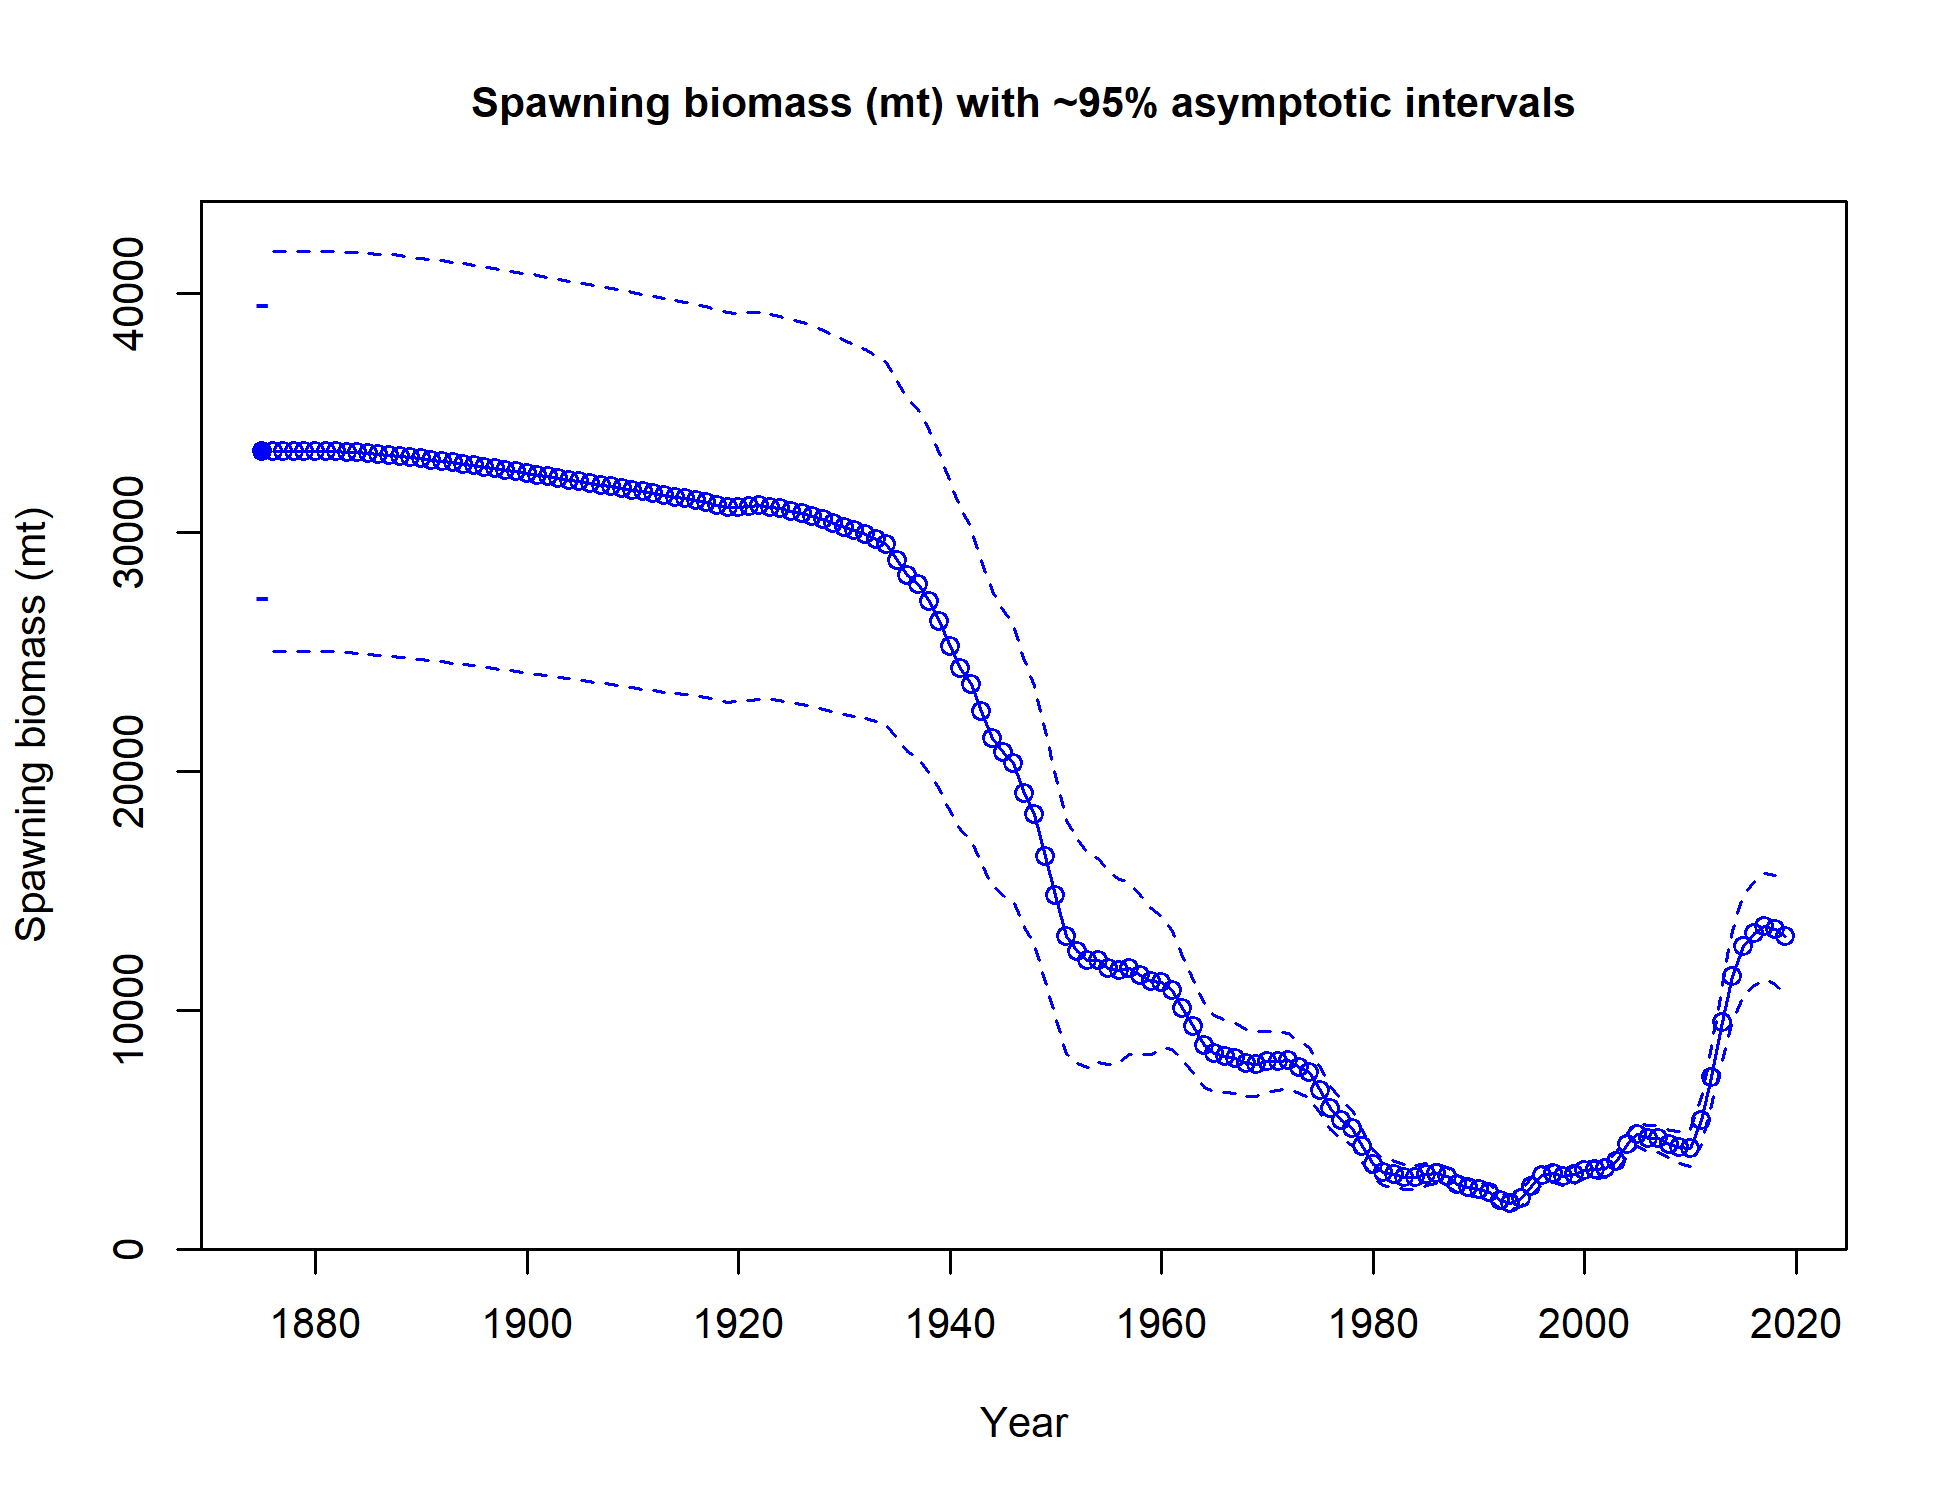
\includegraphics{r4ss/plots_mod1/ts7_Spawning_biomass_(mt)_with_95_asymptotic_intervals_intervals}
\caption{Estimated time-series of spawning output trajectory (circles
and line: median; light broken lines: 95\% credibility intervals) for
Petrale sole. \label{fig:ssb}}
\end{figure}

\FloatBarrier

\begin{figure}
\centering
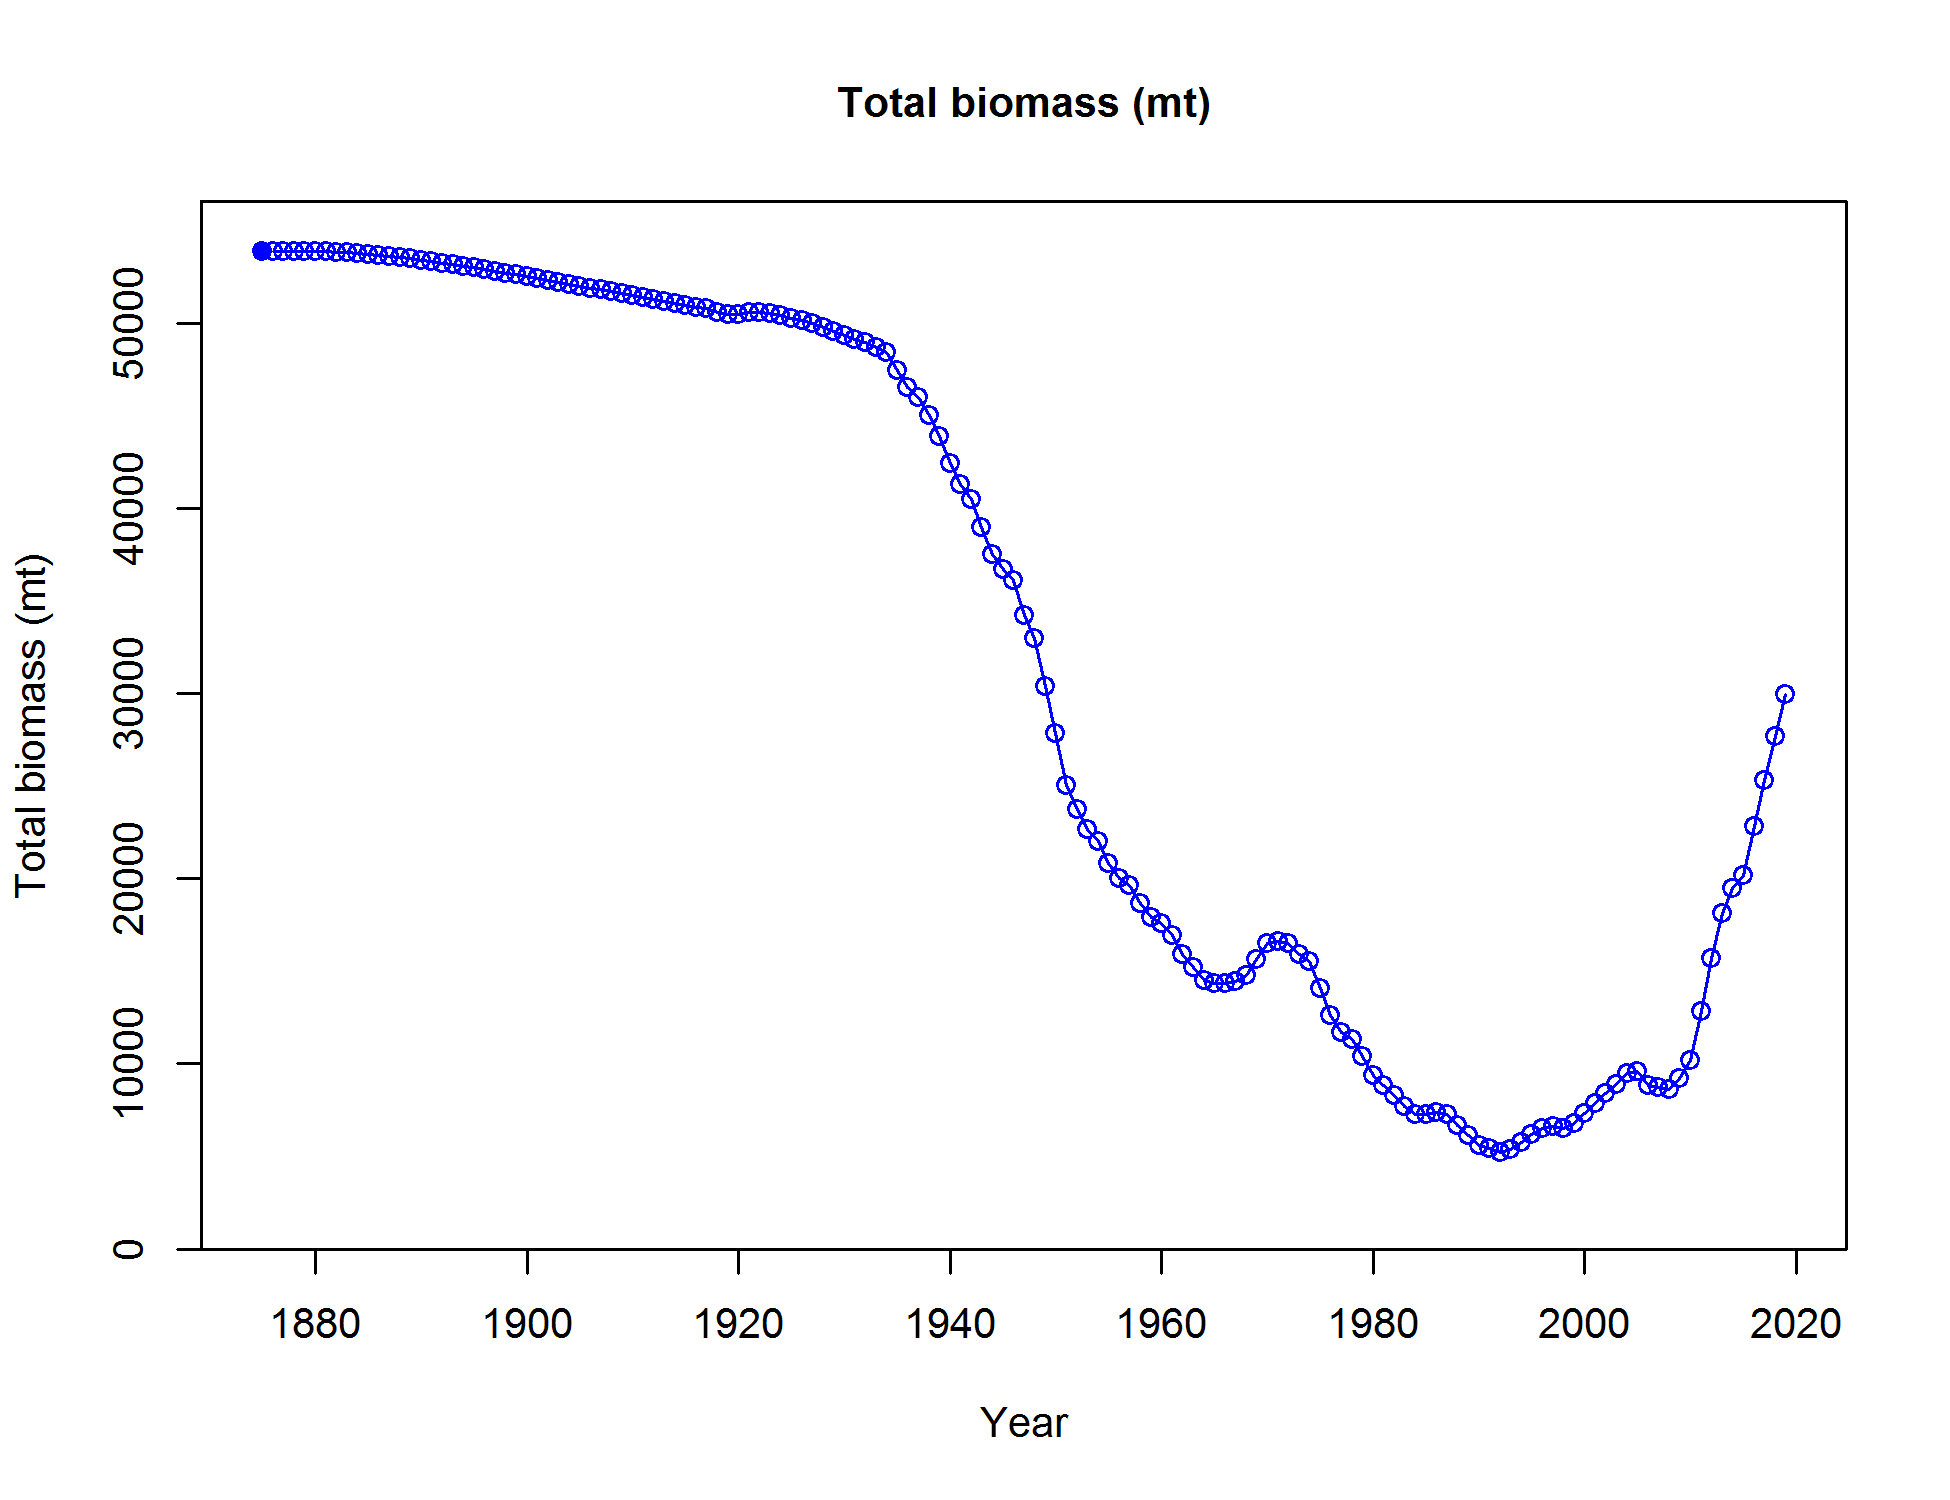
\includegraphics{r4ss/plots_mod1/ts1_Total_biomass_(mt).png}
\caption{Estimated time-series of total biomass for Petrale sole.
\label{fig:total_bio}}
\end{figure}

\FloatBarrier

\begin{figure}
\centering
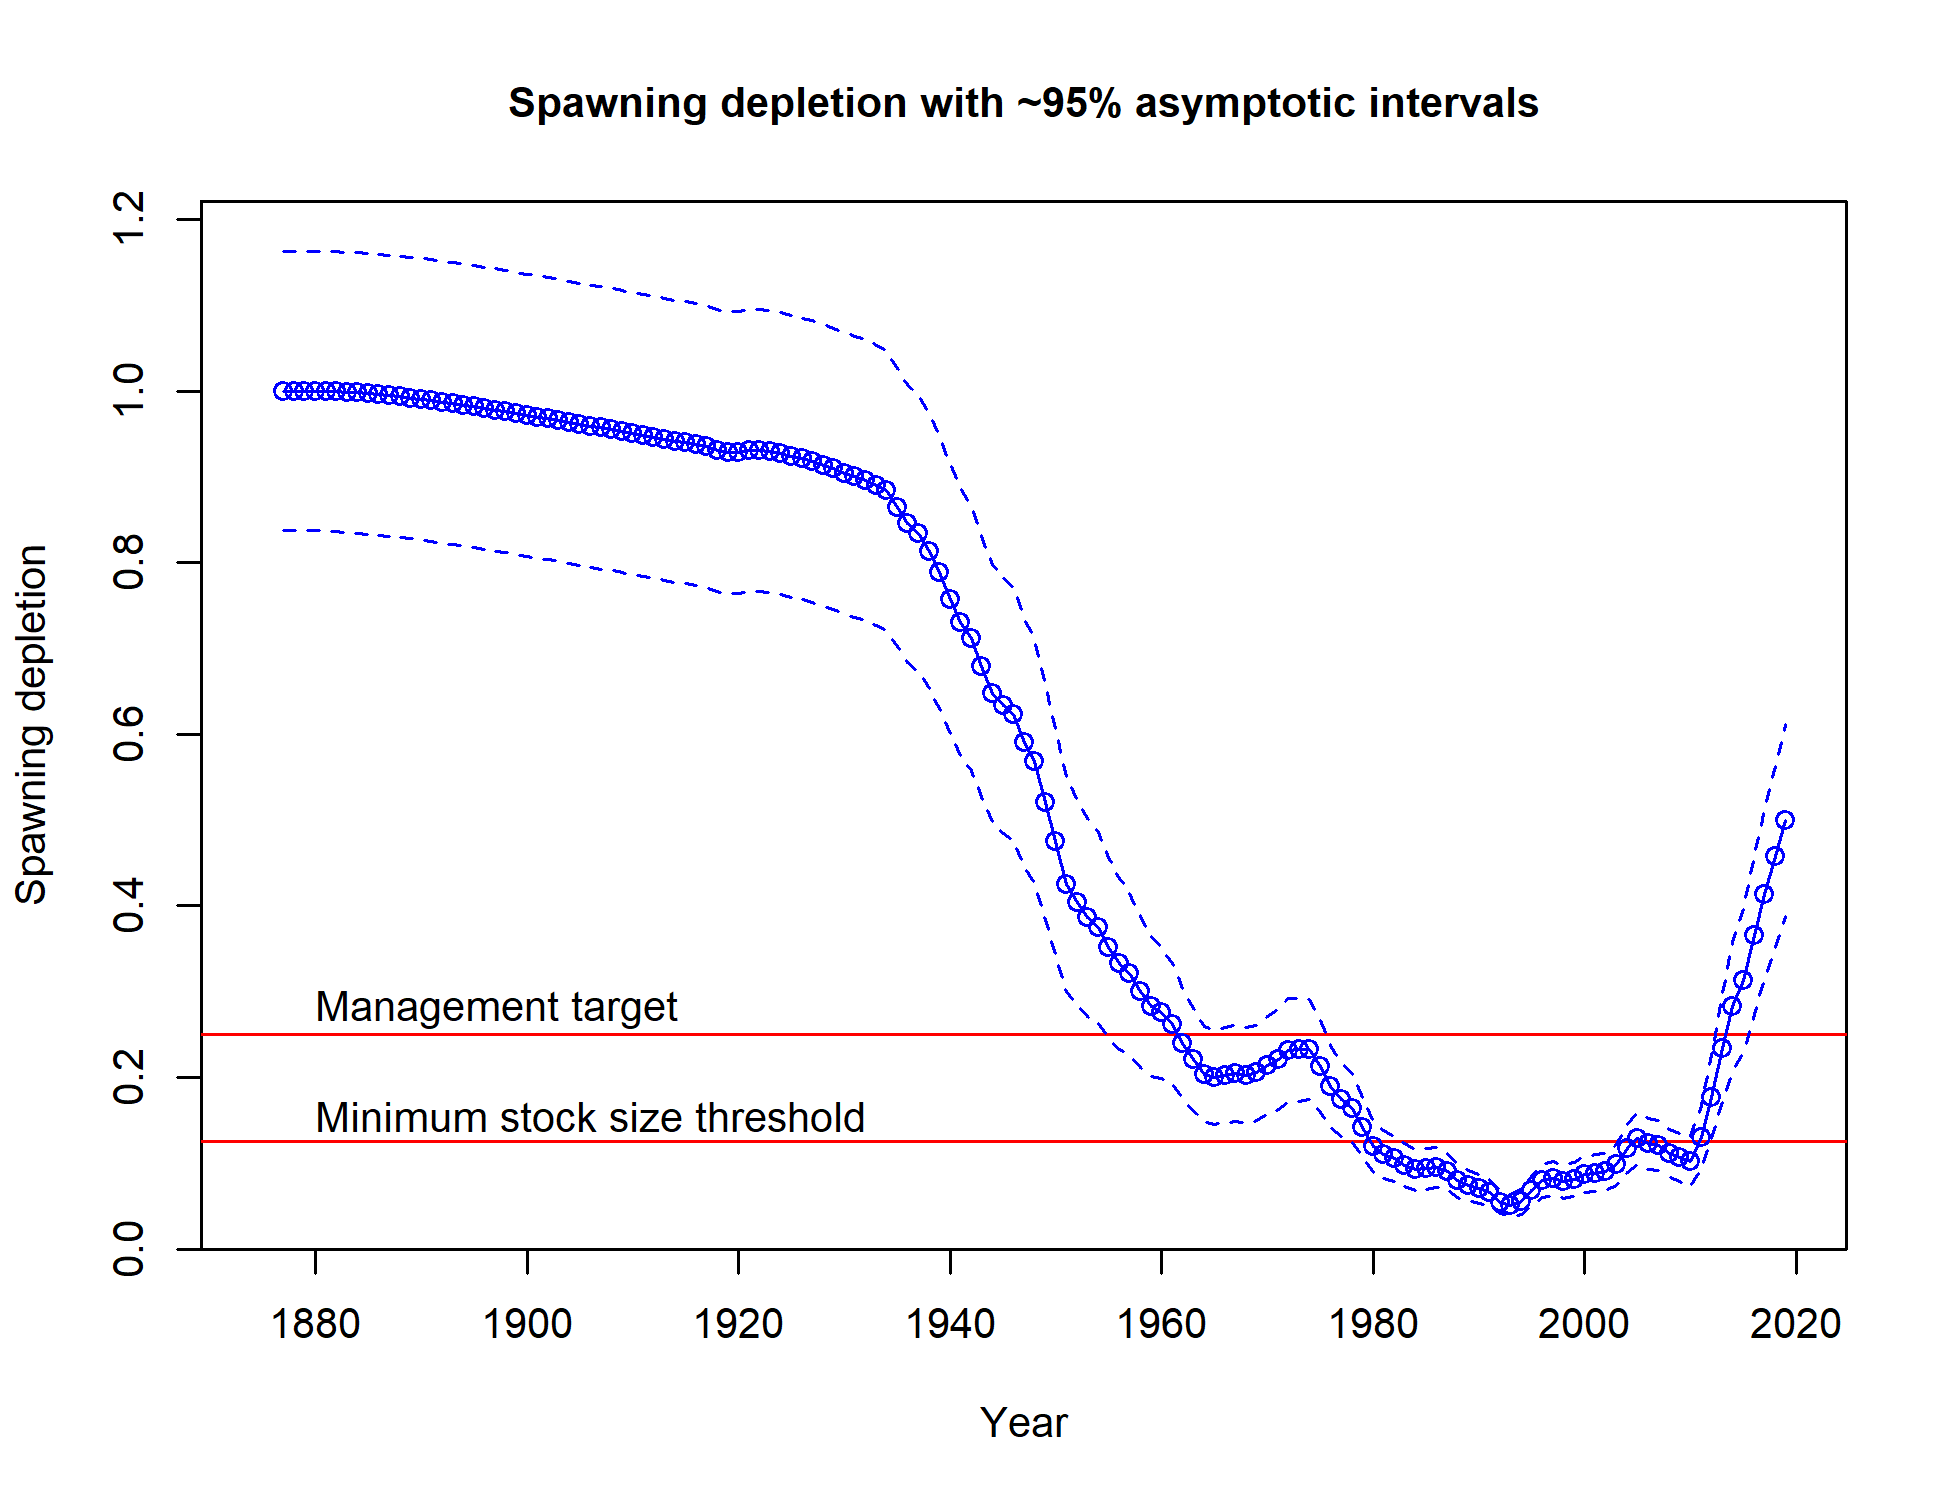
\includegraphics{r4ss/plots_mod1/ts9_Spawning_depletion_with_95_asymptotic_intervals_intervals.png}
\caption{Estimated time-series of relative spawning output (depletion)
(circles and line: median; light broken lines: 95\% credibility
intervals) for Petrale sole. \label{fig:depl}}
\end{figure}

\FloatBarrier

\begin{figure}
\centering
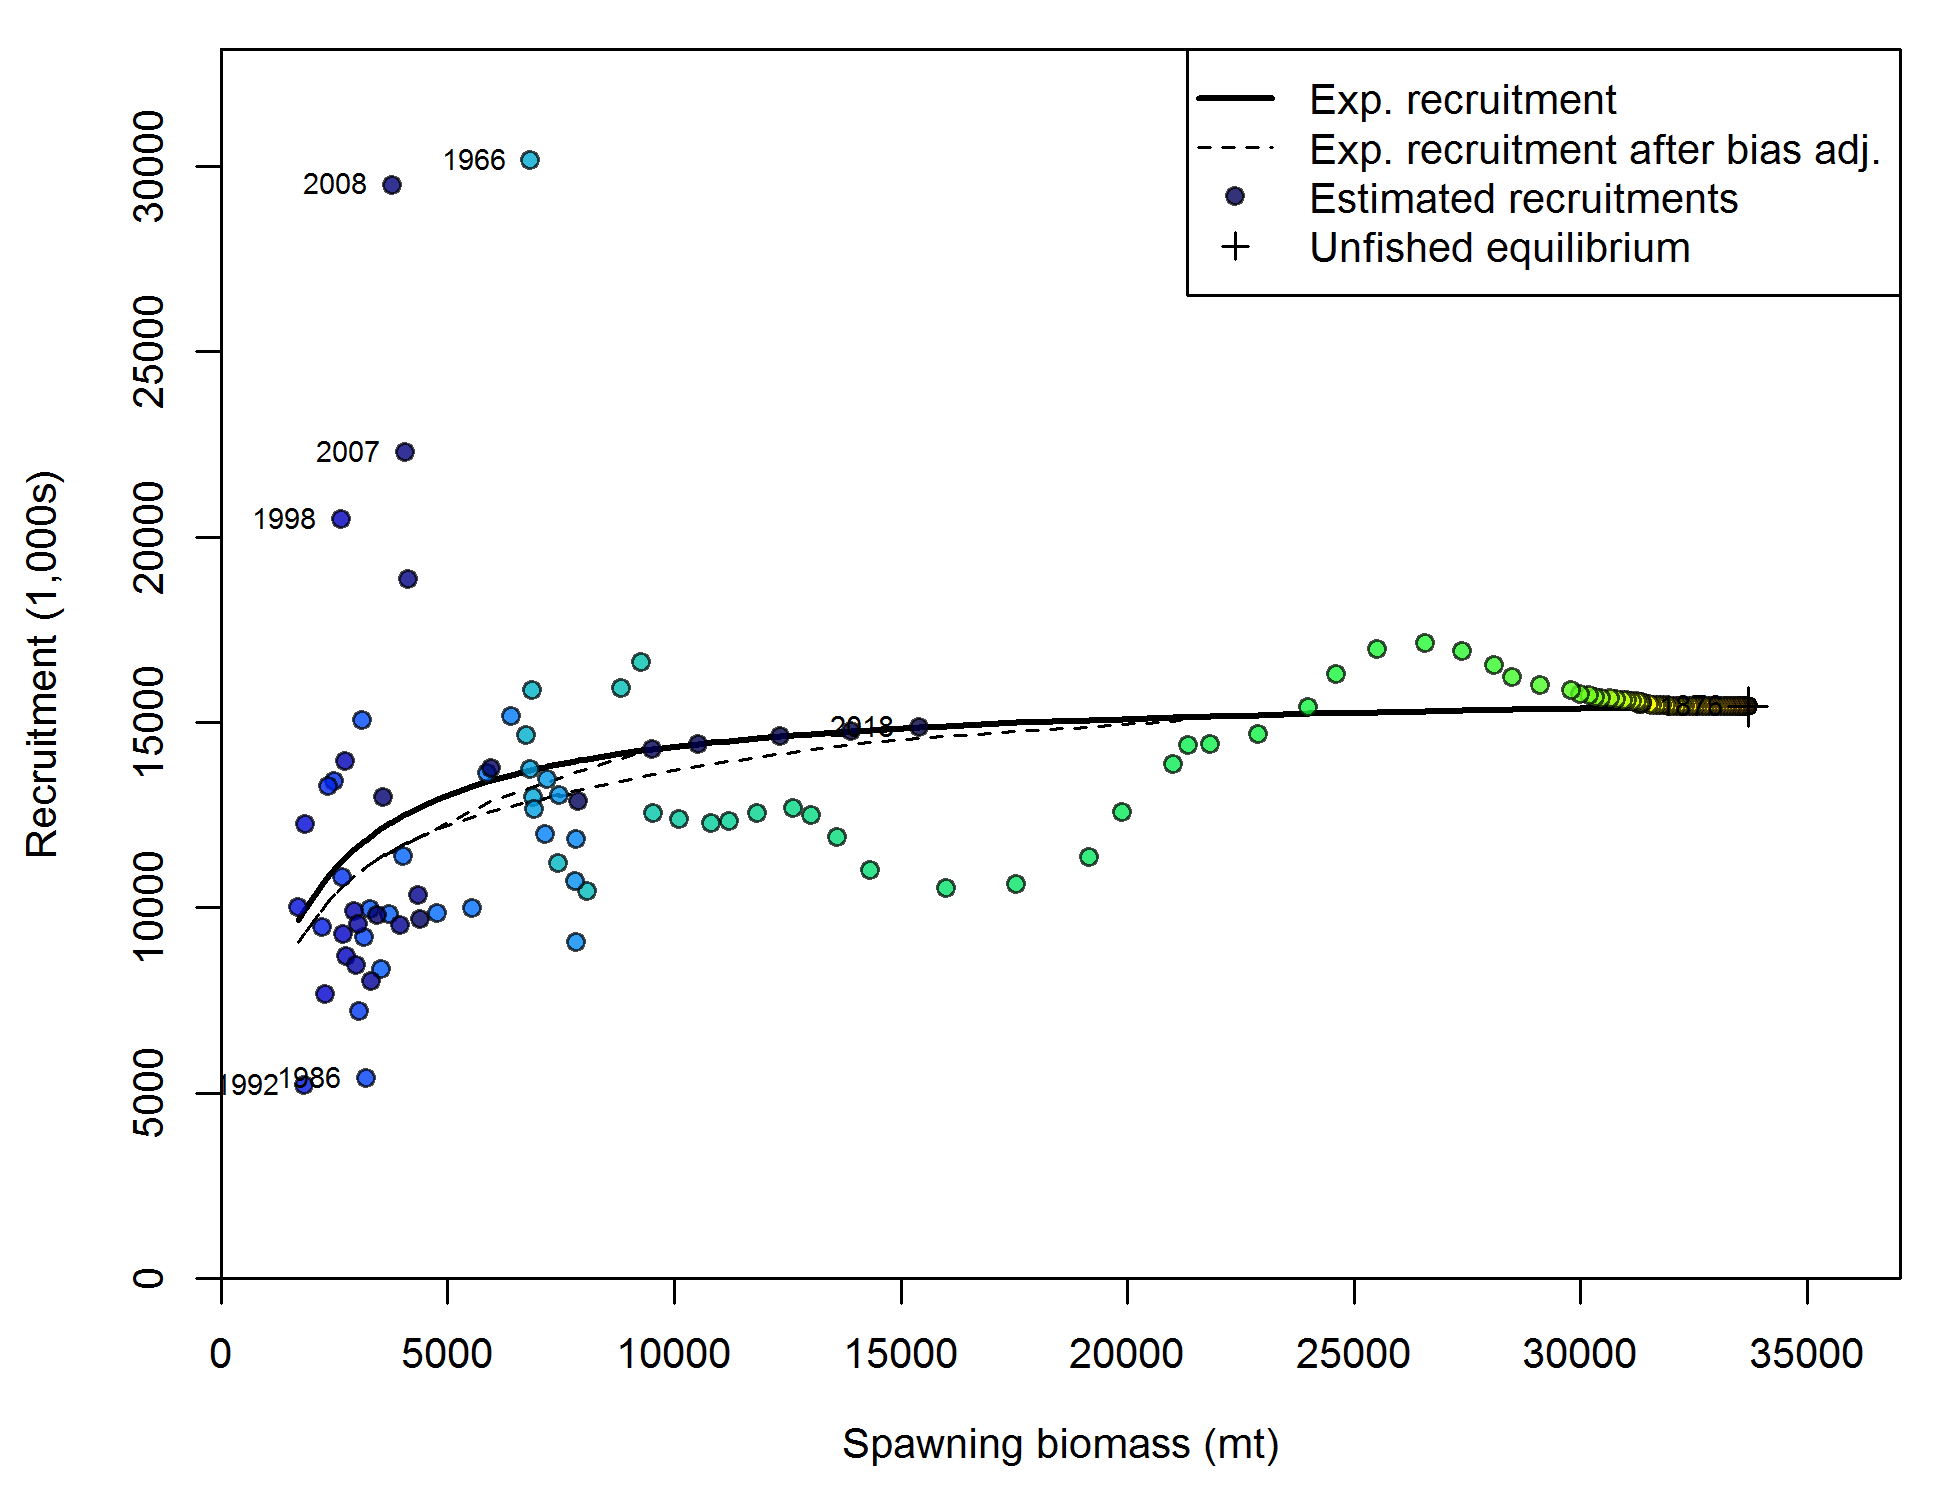
\includegraphics{r4ss/plots_mod1/SR_curve2.png}
\caption{Estimated recruitment (red circles) and the assumed
stock-recruit relationship (black line). The green line shows the effect
of the bias correction for the lognormal distribution
\label{fig:stock_recruit_curve}}
\end{figure}

\begin{figure}
\centering
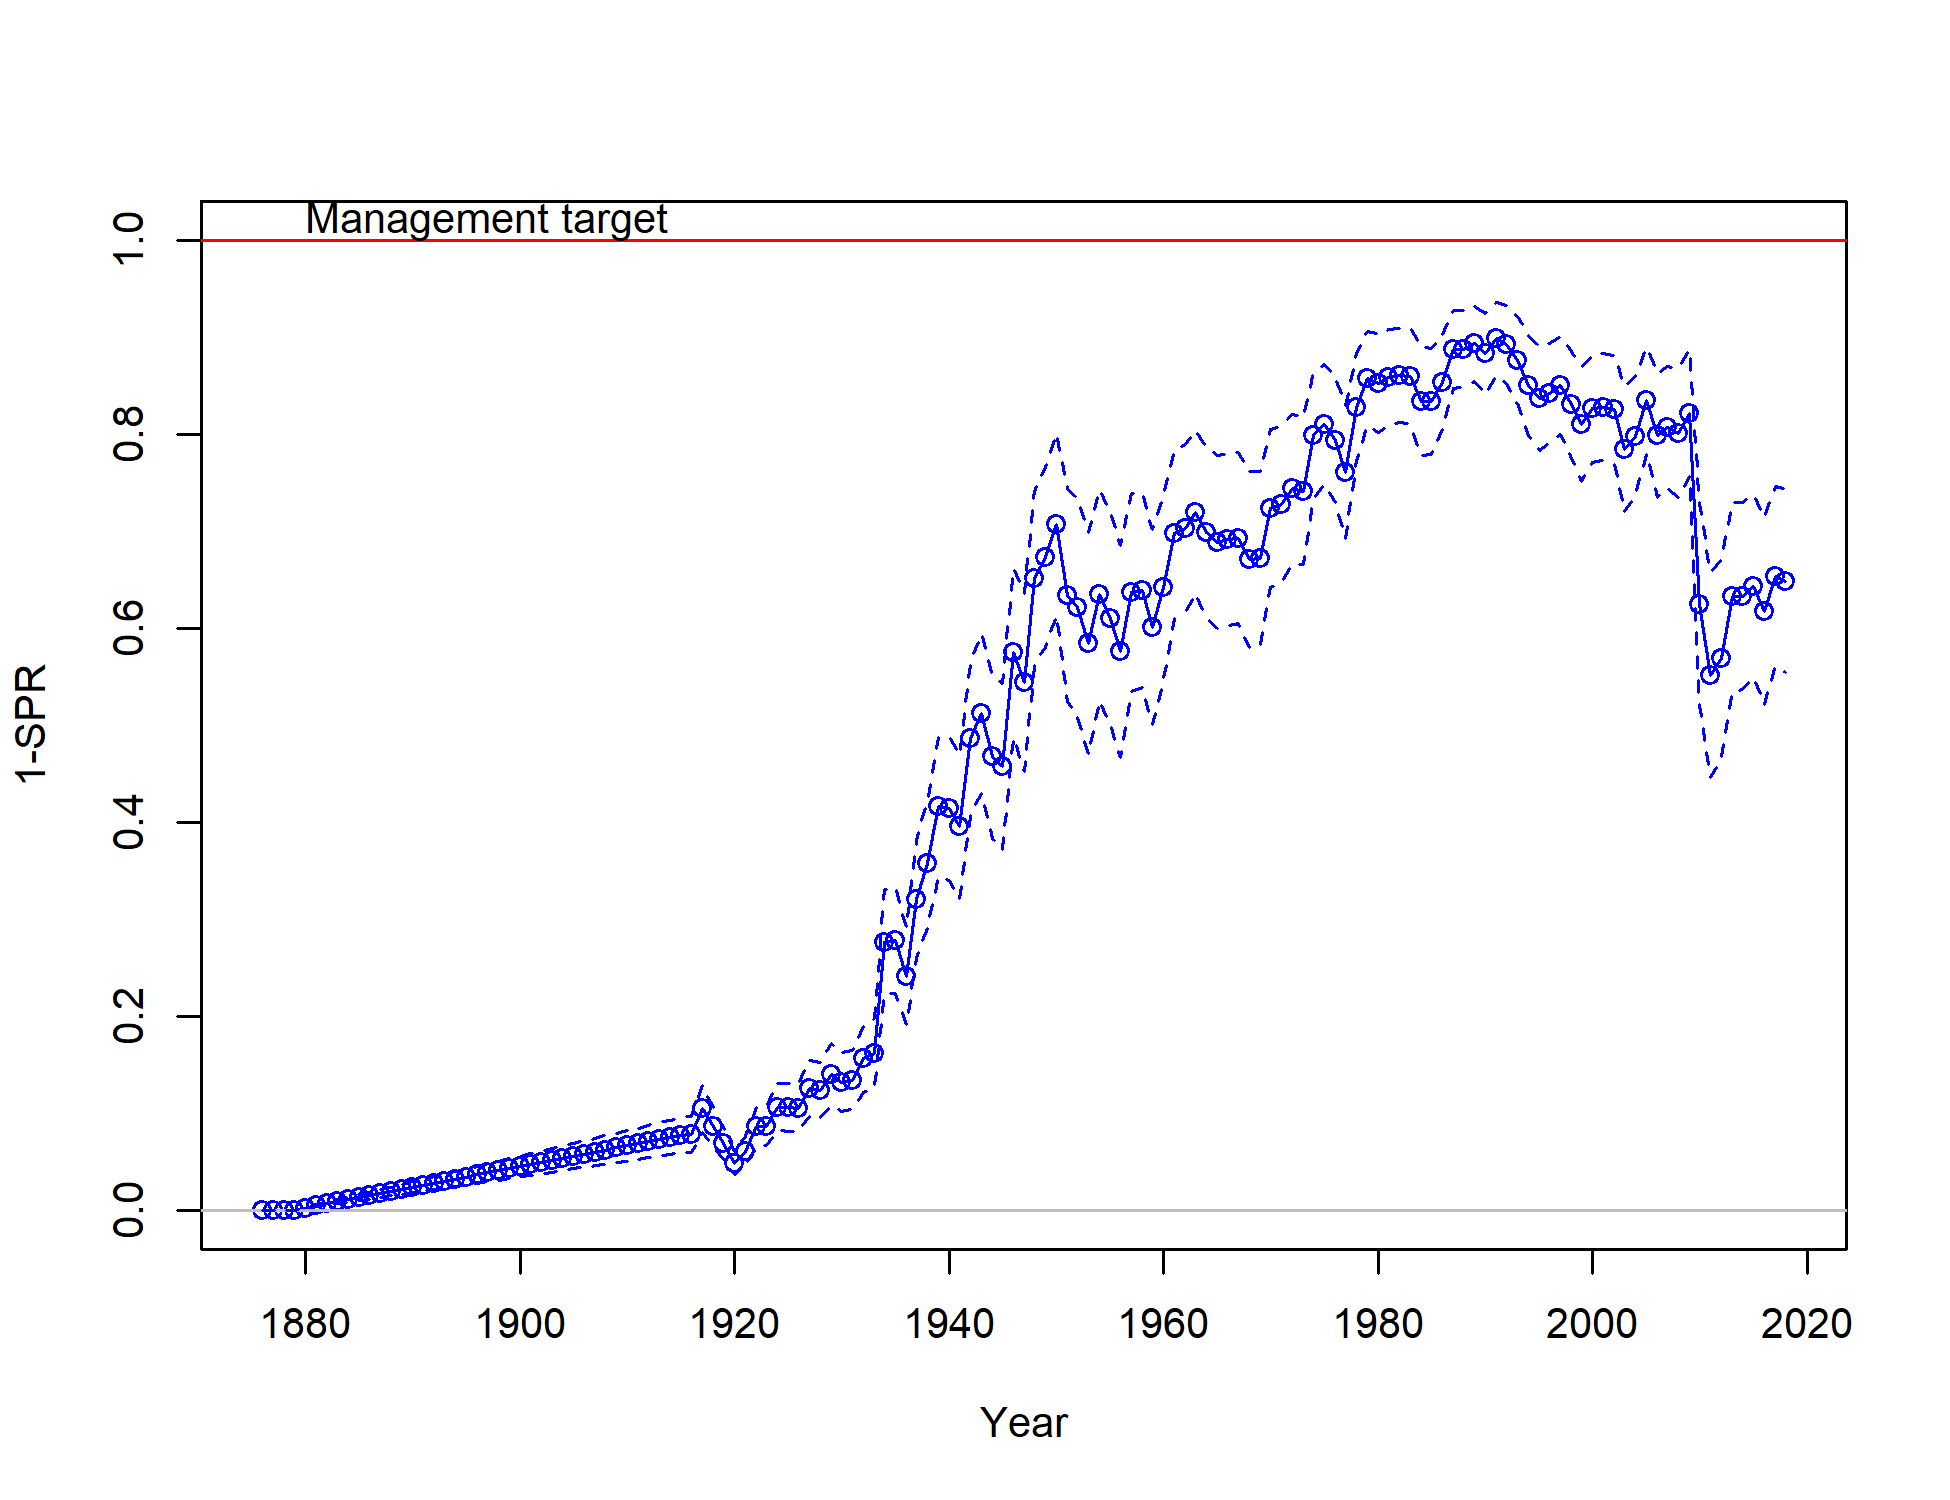
\includegraphics{r4ss/plots_mod1/SPR3_ratiointerval.png}
\caption{Estimated spawning potential ratio (1-SPR)/(1-SPR30\%) for the
base-case model. One minus SPR is plotted so that higher exploitation
rates occur on the upper portion of the y-axis. The management target is
plotted as a red horizontal line and values above this reflect harvests
in excess of the overfishing proxy based on the SPR30\% harvest rate.
The last year in the time series is 2018. \label{fig:SPR}}
\end{figure}

\FloatBarrier

\begin{figure}
\centering
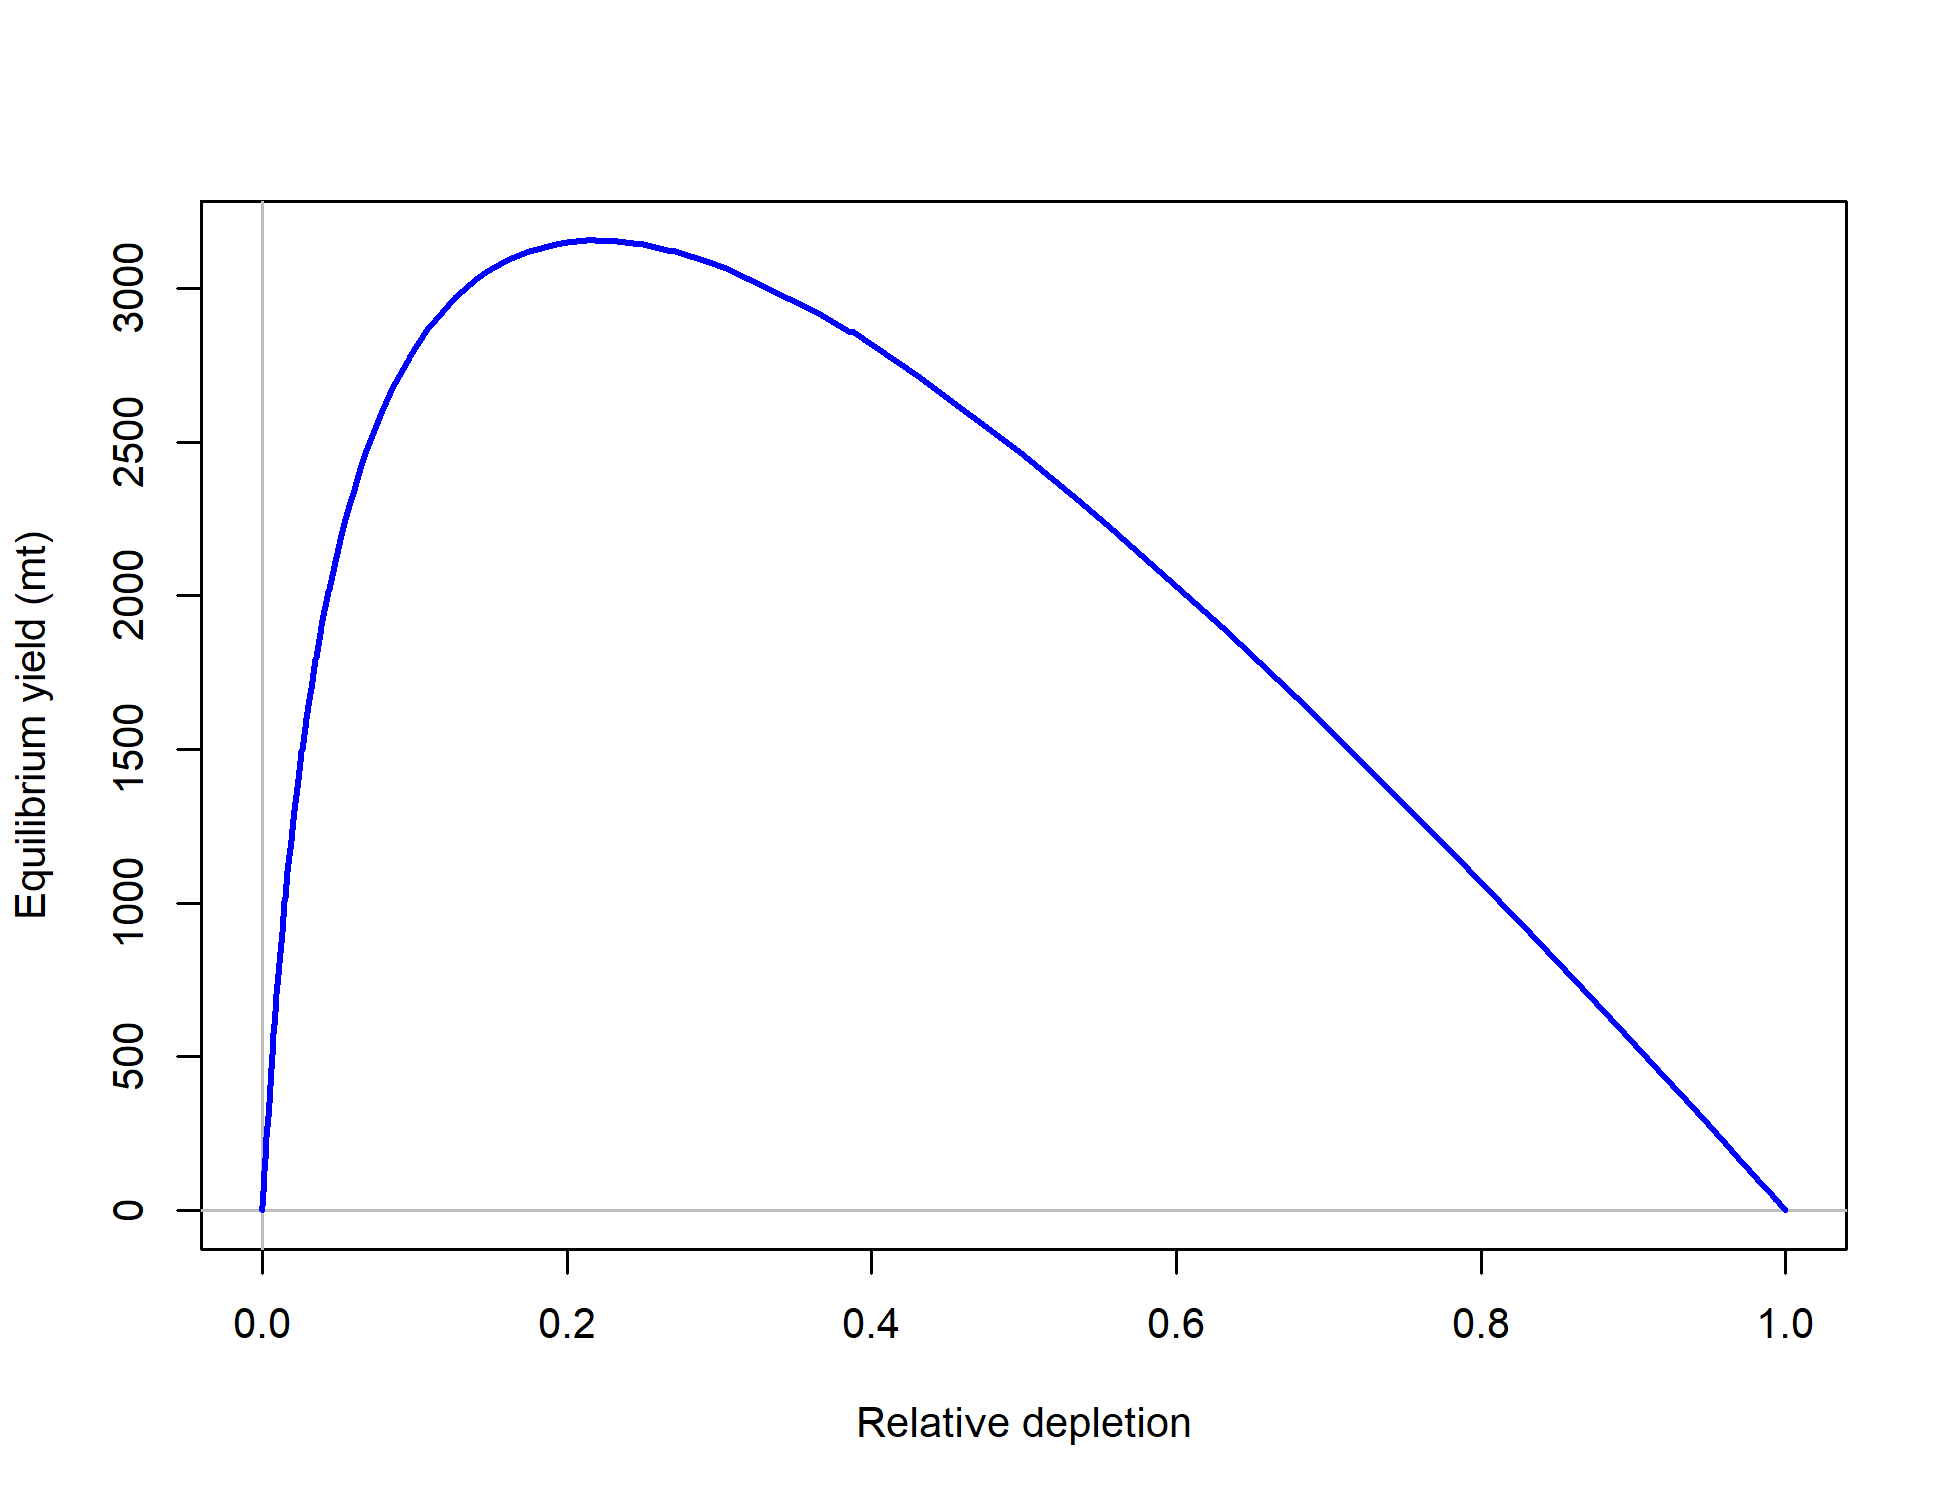
\includegraphics{r4ss/plots_mod1/yield1_yield_curve.png}
\caption{Equilibrium yield curve for the base case model. Values are
based on the 2018 fishery selectivity and with steepness fixed at 0.89.
\label{fig:yield}}
\end{figure}

\FloatBarrier

\newpage

\color{black}

\section{References}\label{references}

\renewcommand{\thepage}{}

\hypertarget{refs}{}
\hypertarget{ref-methot_stock_2013}{}
Methot, R.D., and Wetzel, C.R. 2013. Stock synthesis: A biological and
statistical framework for fish stock assessment and fishery management.
Fisheries Research \textbf{142}: 86--99. doi:
\href{https://doi.org/10.1016/j.fishres.2012.10.012}{10.1016/j.fishres.2012.10.012}.

\hypertarget{ref-pikitch_evaluation_1988}{}
Pikitch, E.K., Erickson, D.L., and Wallace, J.R. 1988. An evaluation of
the effectiveness of trip limits as a management tool. Northwest; Alaska
Fisheries Center, National Marine Fisheries Service NWAFC Processed
Report. Available from
\url{https://www.afsc.noaa.gov/Publications/ProcRpt/PR1988-27.pdf}
{[}accessed 28 February 2017{]}.

\hypertarget{ref-rogers_numerical_1992}{}
Rogers, J.B., and Pikitch, E.K. 1992. Numerical definition of groundfish
assemblages caught off the coasts of Oregon and Washington using
commercial fishing strategies. Canadian Journal of Fisheries and Aquatic
Sciences \textbf{49}(12): 2648--2656.

\hypertarget{ref-weinberg_estimation_2002}{}
Weinberg, J.R., Rago, P.J., Wakefield, W.W., and Keith, C. 2002.
Estimation of tow distance and spatial heterogeneity using data from
inclinometer sensors: An example using a clam survey dredge. Fisheries
Research \textbf{55}(1--3): 49--61. doi:
\href{https://doi.org/10.1016/S0165-7836(01)00292-2}{10.1016/S0165-7836(01)00292-2}.

\end{document}
